%pla% -*- Mode:TeX -*-

%% IMPORTANT: The official thesis specifications are available at:
%%            http://libraries.mit.edu/archives/thesis-specs/
%%
%%            Please verify your thesis' formatting and copyright
%%            assignment before submission.  If you notice any
%%            discrepancies between these templates and the 
%%            MIT Libraries' specs, please let us know
%%            by e-mailing thesis@mit.edu

%% The documentclass options along with the pagestyle can be used to generate
%% a technical report, a draft copy, or a regular thesis.  You may need to
%% re-specify the pagestyle after you \include  cover.tex.  For more
%% information, see the first few lines of mitthesis.cls. 

%\documentclass[12pt,vi,twoside]{mitthesis}
%%
%%  If you want your thesis copyright to you instead of MIT, use the
%%  ``vi'' option, as above.
%%
%\documentclass[12pt,twoside,leftblank]{mitthesis}
%%
%% If you want blank pages before new chapters to be labelled ``This
%% Page Intentionally Left Blank'', use the ``leftblank'' option, as
%% above. 	

\documentclass[12pt,doublespacing]{mitthesis}
\usepackage{setspace}
\usepackage{lgrind}
\usepackage{graphicx}
\usepackage{float}
\usepackage{placeins}
\usepackage{cite}
\usepackage[utf8x]{inputenc}
\usepackage{wrapfig}
\usepackage{amsmath,varwidth,array,ragged2e}
\usepackage{amsbsy}
\usepackage{paralist}
\usepackage{amssymb}
\usepackage{caption}
\usepackage{listings}
\usepackage{epigraph}
\usepackage{quotchap}
\usepackage{color}
\usepackage{url}
\usepackage{mdframed}
\usepackage{color}
\usepackage{hyperref}
\pagestyle{plain}
\usepackage{paralist}
\usepackage{algorithm}
\usepackage{algorithmic}
\usepackage[cmtip,all]{xy}
\usepackage{mathtools}
\usepackage{graphicx, subfigure}
\usepackage{cases}
\usepackage{fullpage}
\usepackage{subfigure}
\usepackage{placeins}
\usepackage{tikz}
\usepackage{calligra} % for dedication
\usepackage[percent]{overpic}
\usepackage[english]{babel}
\usepackage{wrapfig,lipsum,booktabs}
\usepackage{colortbl}
\usepackage{tocvsec2}
\usepackage{multirow}
\usepackage{longtable}
\definecolor{Gray}{gray}{0.85}
\definecolor{LightCyan}{rgb}{0.88,1,1}




%\onehalfspacing
%% This bit allows you to either specify only the files which you wish to
%% process, or `all' to process all files which you \include.
%% Krishna Sethuraman (1990).
\usepackage{tikz}
\usetikzlibrary{matrix}
\usepackage[nottoc]{tocbibind}
\usepackage[left=3.5cm,top=2.5cm,right=2.2cm,bottom=3.1cm,bindingoffset=0.5cm]{geometry}
 


\DeclarePairedDelimiter\ceil{\lceil}{\rceil}
\DeclarePairedDelimiter\floor{\lfloor}{\rfloor}
\begin{document}


% -*-latex-*-
% 
% For questions, comments, concerns or complaints:
% thesis@mit.edu
% 
%
% $Log: cover.tex,v $
% Revision 1.8  2008/05/13 15:02:15  jdreed
% Degree month is June, not May.  Added note about prevdegrees.
% Arthur Smith's title updated
%
% Revision 1.7  2001/02/08 18:53:16  boojum
% changed some \newpages to \cleardoublepages
%
% Revision 1.6  1999/10/21 14:49:31  boojum
% changed comment referring to documentstyle
%
% Revision 1.5  1999/10/21 14:39:04  boojum
% *** empty log message ***
%
% Revision 1.4  1997/04/18  17:54:10  othomas
% added page numbers on abstract and cover, and made 1 abstract
% page the default rather than 2.  (anne hunter tells me this
% is the new institute standard.)
%
% Revision 1.4  1997/04/18  17:54:10  othomas
% added page numbers on abstract and cover, and made 1 abstract
% page the default rather than 2.  (anne hunter tells me this
% is the new institute standard.)
%
% Revision 1.3  93/05/17  17:06:29  starflt
% Added acknowledgements section (suggested by tompalka)
% 
% Revision 1.2  92/04/22  13:13:13  epeisach
% Fixes for 1991 course 6 requirements
% Phrase "and to grant others the right to do so" has been added to 
% permission clause
% Second copy of abstract is not counted as separate pages so numbering works
% out
% 
% Revision 1.1  92/04/22  13:08:20  epeisach

% NOTE:
% These templates make an effort to conform to the MIT Thesis specifications,
% however the specifications can change.  We recommend that you verify the
% layout of your title page with your thesis advisor and/or the MIT 
% Libraries before printing your final copy.
\title{Accelerating the new SCIARA-fv3 numerical model by different GPGPU
strategies}


\author{Davide Spataro}
% If you wish to list your previous degrees on the cover page, use the 
% previous degrees command:
       \prevdegrees{B.S., Universit\`a della Calabria (2011)}
% You can use the \\ command to list multiple previous degrees
%       \prevdegrees{B.S., University of California (1978) \\
%                    S.M., Massachusetts Institute of Technology (1981)}
\department{Department of Mathematics and Computer Science}

% If the thesis is for two degrees simultaneously, list them both
% separated by \and like this:
% \degree{Doctor of Philosophy \and Master of Science}
\degree{Master of Science}

% As of the 2007-08 academic year, valid degree months are September, 
% February, or June.  The default is June.
\degreemonth{July}
\degreeyear{2014}
\thesisdate{July 27, 2014}

%% By default, the thesis will be copyrighted to MIT.  If you need to copyright
%% the thesis to yourself, just specify the `vi' documentclass option.  If for
%% some reason you want to exactly specify the copyright notice text, you can
%% use the \copyrightnoticetext command.  
\copyrightnoticetext{\copyright Universit\`a della Calabria, 2014. All right
reserved}

% If there is more than one supervisor, use the \supervisor command
% once for each.
\supervisor{Wylliam Spataro}{Associate Professor}
\supervisor{Donato D'Ambrosio}{Associate Professor}

% This is the department committee chairman, not the thesis committee
% chairman.  You should replace this with your Department's Committee
% Chairman.
\chairman{Nicola Leone}{Chairman, Department Committee on Graduate Theses}

% Make the titlepage based on the above information.  If you need
% something special and can't use the standard form, you can specify
% the exact text of the titlepage yourself.  Put it in a titlepage
% environment and leave blank lines where you want vertical space.
% The spaces will be adjusted to fill the entire page.  The dotted
% lines for the signatures are made with the \signature command.
\maketitle
 \pagestyle{empty}
\newpage \vspace*{7cm} \hspace*{12cm}
\pdfbookmark[0]{Dedication}{dedication} % Sets a PDF bookmark for the dedication
{\large \textit{Alla mia famiglia.}}
\par
\hspace*{12cm}
\large \textit{A Maria.}


% The abstractpage environment sets up everything on the page except
% the text itself.  The title and other header material are put at the
% top of the page, and the supervisors are listed at the bottom.  A
% new page is begun both before and after.  Of course, an abstract may
% be more than one page itself.  If you need more control over the
% format of the page, you can use the abstract environment, which puts
% the word "Abstract" at the beginning and single spaces its text.

%% You can either \input (*not* \include) your abstract file, or you can put
%% the text of the abstract directly between the \begin{abstractpage} and
%% \end{abstractpage} commands.

% First copy: start a new page, and save the page number.
\cleardoublepage
% Uncomment the next line if you do NOT want a page number on your
% abstract and acknowledgments pages.
 \pagestyle{empty}
\setcounter{savepage}{\thepage}
\begin{abstractpage}
% $Log: abstract.tex,v $ Revision 1.1  93/05/14  14:56:25  starflt Initial
% revision  Revision 1.1  90/05/04  10:41:01  lwvanels Initial revision   % The
% text of your abstract and nothing else (other than comments) goes here.
% % It will be single-spaced and the rest of the text that is supposed to go on
% % the abstract page will be generated by the abstractpage environment.  This %
% file should be \input (not \include 'd) from cover.tex.
\hfill \\
\textit{\textbf{English}}   \hfill \\
\hfill \\
 In
this thesis, a parallel version of the model SCIARA-fv3\cite{Spataro2010} was
designed and implemented using General-Purpose Computation with Graphics
Processing Units (GPGPU) and specifically, by adopting the NVIDIA Compute
Unified Device Architecture (CUDA)\cite{NvidiaprogGuide} framework in order to
improve the overall execution time. It involves the design and the application
of strategies that allow to avoid incorrect computation results due to race
conditions of any type and at the same time to achieve the best performance and
occupancy of the underlying available hardware. Carried out experiments show
that significant performance improvement in terms of speedup are achieved also
thanks to some original optimizations strategies adopted, confirming the
validity of graphics hardware as an alternative to much more expensive solutions
for the simulation of cellular automata models.
\hfill \\
\begin{center}
\line(1,0){350} \hfill \\
\end{center}
\hfill \\
\hfill \\
\textit{\textbf{Italian}}   \hfill \\
\hfill \\


In questo lavoro di tesi ho progettato ed implementato una versione parallela
del modello numero SCIARA-fv3\cite{Spataro2010} utilizzando le schede grafiche
per il calcolo general-purpose (General Purpose Computation with Graphics
Processing Units - GPGPU), adottando il  Compute Unified Device Architecture (CUDA)\cite{NvidiaprogGuide} framework
di NVIDIA con lo scopo di migliorare i tempi di esecuzione complessivi.
Questo ha comportato il design prima, e l'applicazione vera e propria poi, di
strategie che permettessero sia di evitare errori dovuti a race-conditions di
qualsiasi tipo che di raggiungere gli speedups migliori con l'hardware a
disposizione. Gli esperimenti effettuati mostrano significativi miglioramenti
nelle performance in termini di speedup grazie anche all'utilizzo di alcune stragie d'ottimizzazione nuove,
confermando la validit\`a dell'uso di processori grafici come alternativa a
soluzioni hardware per la parallelizzazione di modelli ad
automi cellulari molto pi\`u costose.




\end{abstractpage}



% Additional copy: start a new page, and reset the page number.  This way,
% the second copy of the abstract is not counted as separate pages.
% Uncomment the next 6 lines if you need two copies of the abstract
% page.
% \setcounter{page}{\thesavepage}
% \begin{abstractpage}
% % $Log: abstract.tex,v $ Revision 1.1  93/05/14  14:56:25  starflt Initial
% revision  Revision 1.1  90/05/04  10:41:01  lwvanels Initial revision   % The
% text of your abstract and nothing else (other than comments) goes here.
% % It will be single-spaced and the rest of the text that is supposed to go on
% % the abstract page will be generated by the abstractpage environment.  This %
% file should be \input (not \include 'd) from cover.tex.
\hfill \\
\textit{\textbf{English}}   \hfill \\
\hfill \\
 In
this thesis, a parallel version of the model SCIARA-fv3\cite{Spataro2010} was
designed and implemented using General-Purpose Computation with Graphics
Processing Units (GPGPU) and specifically, by adopting the NVIDIA Compute
Unified Device Architecture (CUDA)\cite{NvidiaprogGuide} framework in order to
improve the overall execution time. It involves the design and the application
of strategies that allow to avoid incorrect computation results due to race
conditions of any type and at the same time to achieve the best performance and
occupancy of the underlying available hardware. Carried out experiments show
that significant performance improvement in terms of speedup are achieved also
thanks to some original optimizations strategies adopted, confirming the
validity of graphics hardware as an alternative to much more expensive solutions
for the simulation of cellular automata models.
\hfill \\
\begin{center}
\line(1,0){350} \hfill \\
\end{center}
\hfill \\
\hfill \\
\textit{\textbf{Italian}}   \hfill \\
\hfill \\


In questo lavoro di tesi ho progettato ed implementato una versione parallela
del modello numero SCIARA-fv3\cite{Spataro2010} utilizzando le schede grafiche
per il calcolo general-purpose (General Purpose Computation with Graphics
Processing Units - GPGPU), adottando il  Compute Unified Device Architecture (CUDA)\cite{NvidiaprogGuide} framework
di NVIDIA con lo scopo di migliorare i tempi di esecuzione complessivi.
Questo ha comportato il design prima, e l'applicazione vera e propria poi, di
strategie che permettessero sia di evitare errori dovuti a race-conditions di
qualsiasi tipo che di raggiungere gli speedups migliori con l'hardware a
disposizione. Gli esperimenti effettuati mostrano significativi miglioramenti
nelle performance in termini di speedup grazie anche all'utilizzo di alcune stragie d'ottimizzazione nuove,
confermando la validit\`a dell'uso di processori grafici come alternativa a
soluzioni hardware per la parallelizzazione di modelli ad
automi cellulari molto pi\`u costose.




% \end{abstractpage}

\cleardoublepage

\section*{Acknowledgments}

This thesis would not have been possible without the help, support and patience
of my principal supervisors, Prof.~\textit{William Spataro}
and \textit{Donato D'Ambrosio}.

The good advices and support of Dr. \textit{Giuseppe Filippone} have been
invaluable on both  academic and  personal level, for which I am extremely grateful.



I would like to acknowledge the technical and academic support of the Prof.
\textit{Davide Marocco} from  \textit{Plymouth University}, particularly for
providing  all the necessary hardware for this research and for
enabling me to take part to this great experience in United Kingdom.

The \textit{Universit\`a della Calabria} for
sponsoring me with a Erasmus Placement studentship.

All the researcher in the \textit{School of Computing and Mathematics of the
Plymouth University}, particularly those who work in the \textit{Centre for
Robotics and Neural Systems (CRNS)} for promoting a stimulating and welcoming academic and
social environment will stand as an example to those that succeed them.

I must also acknowledge Dr. \textit{Valerio Biscione} from \textit{University
of Plymouth}  for his suggestions, motivation and  encouragement.\@



\newpage



%%%%%%%%%%%%%%%%%%%%%%%%%%%%%%%%%%%%%%%%%%%%%%%%%%%%%%%%%%%%%%%%%%%%%%
% -*-latex-*-

% Some departments (e.g. 5) require an additional signature page.  See
% signature.tex for more information and uncomment the following line if
% applicable.

\pagestyle{plain}
\setcounter{tocdepth}{5}
\setstretch{1.05}

%\addcontentsline{toc}{section}{\listfigurename}
%\addcontentsline{toc}{section}{\listtablename}
\tableofcontents



\newpage
\chapter{Parallel computing architectures}\label{chap:parallelArchitectures}
                                                                                                                                                                                                                                                                                                                                                                                                                                                                                                                                                                                                                                                                                                                                                                                                                                                                                                                                                                                                                                                                                                                                                                                                                                                                                                                                                                                                                                                                                                                                                                                                                                                                                                                                                                                                                                                                                                                                                                                                                                                                                                                                                                                                                                                                                                                                                                                                                                                                                                                                                                                                                                                                                                                                                                                                                                                                                                                                                              
\section{Introduction}
Parallel computing has a tremendous impact on  various areas, raging from
scientific computation or simulation, commercial and industrial application and
data mining. Lot of effort has put during these years in order to try to
mitigate and overcome the limits regarding the sequential computer architecture.
In particular sequential architecture consist of three main components:
\begin{enumerate}
  \item Processor
  \item Memory
  \item Communication system (datapaths, usually buses)
\end{enumerate}
All three components present bottlenecks that limit the overall computing rate
of a system. Caches, low-latency high bandwidth and small capacity storage, for
example can hide latency of DRAM chips storing the fetched data and serving
subsequent requests of the same memory location\footnote{The fraction of the
data satisfied by the cache is called \textit{\textbf{hit rate}}.}. But one of
the most important innovation that addresses these bottlenecks is multiplicity
(in processor, memories and  dataphats) that allows to extend the class of
tractable problems with larger instances and more cases that can be handled. It
is so popular that even smartphones are multicore; Iphone 4S is 2-core, and nexus 4 is 4-core.
This multiplicity has been organized in several manners during
the years giving birth to a variety of architectures. Here a brief classification of the
most important ones.

\section{Architectures}
Classifying a parallel system is not a trivial task. Lots of definitions and
classifications have been proposed in years, mostly based on their hardware
configuration or logical approach in handling and implementing the parallelism.
\subsection{Classical classification - Flynn's taxonomy}
The classification is based on the notion of  \textit{stream of information}.
Two types of information flow into the processor: instructions and data.
Conceptually they can be separated into two independent streams. A coarse
classification can be made taking in account only the number of instructions and
 data streams that a parallel machine can manage (see figure \ref{fig:parallelClassification1}).
That's how Flynn's taxonomy\cite{Flynn1972} classifies machines: according to
whether they have one or more streams of each type.

\begin{figure}
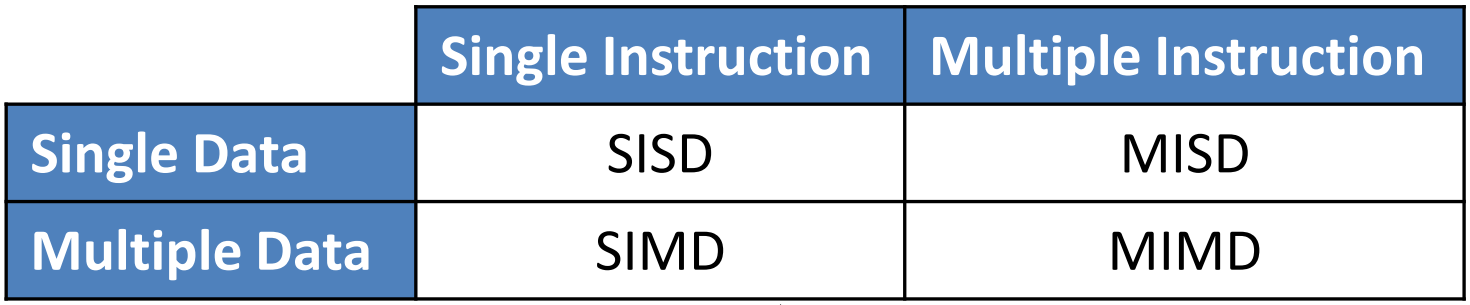
\includegraphics[scale=0.28]{./images/parallelClassification}
\caption[Parallel architecture classification]{Parallel architecture
classification.}
\label{fig:parallelClassification1}
\end{figure}


\begin{description}
\item[SISD:] \textit{\textbf{Single}} instruction \textit{\textbf{Single}}
data.\hfill\\
No parallelism in either instruction or data streams. Each arithmetic
instruction initiates an operation on a data item taken from a single stream of data elements (e.g. mainframes)
\item[SIMD:] \textit{\textbf{Single}} instruction
\textit{\textbf{Multiple}} data. \hfill \\ Data parallelism. The same
instruction is executed on a batch of different data. The control unit is
responsible for fetching and interpreting instructions. When it encounters an
arithmetic or other data processing instruction, it broadcasts the instruction
to all processing elements (PE), which then all perform the same operation. For
example, the instruction might be \textit{add R3,R0.}. Each PE would add the
contents of its own internal register R3 to its own R0. (e.g. stream
processors\footnote{Vector processing is performed on an SIMD machine by distributing
elements of vectors across all data memories.}.)
\item[MISD:] \textit{\textbf{Multiple}} instruction
\textit{\textbf{Single}} data. \hfill \\ Multiple instruction operating on the
same data stream. It is a class of system very unusual, mostly for fault-tolerance reasons.
\item[MIMD:] \textit{\textbf{Multiple}} instruction
\textit{\textbf{Multiple}} data. \hfill \\ Multiple instruction operating
independently on multiple data streams.
(e.g. most modern computers)
\end{description}



\subsection{Memory classification}
Architectures can be further organized by memory architecture and software
models. 
A first rough categorization can be obtained analyzing the memory layout:

\begin{figure}
\centering
\caption{Distributed memory architecture.}
\label{fig:distribuiteMemory}
\setlength{\fboxrule}{1pt}%
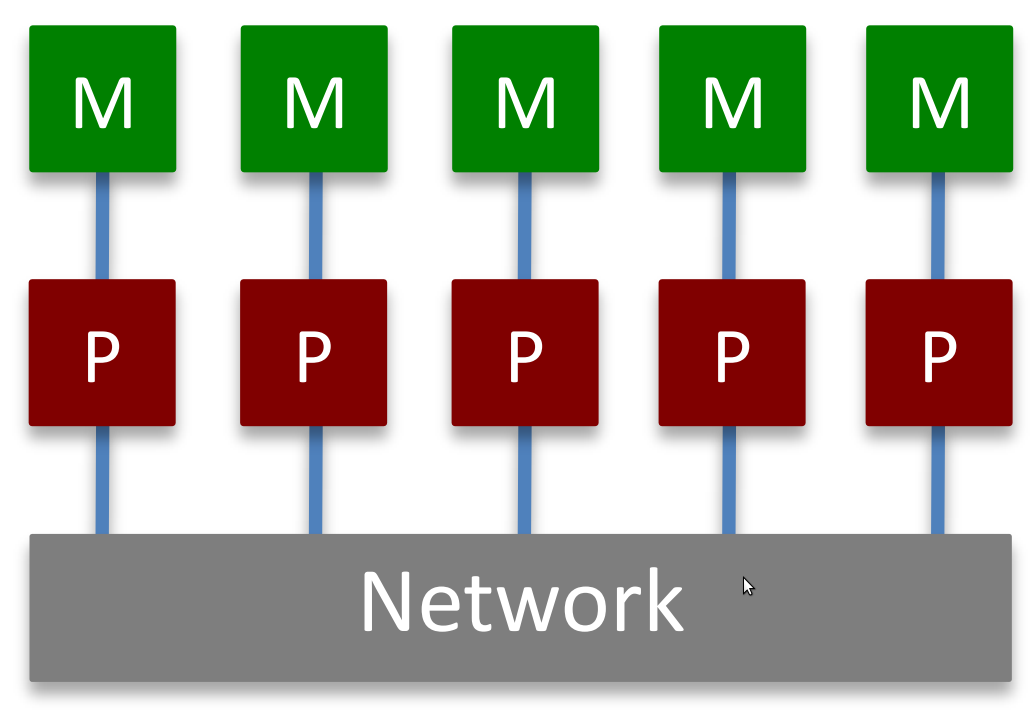
\includegraphics[scale=0.25]{./images/distribuitedMemory}
\end{figure}

\begin{description}
\item[Shared memory] \hfill \\ 
All the processors have in common the ability to access
all memory locations as global space, usually sharing them  via buses. Changes
in memory effected by one processor are visible to all the others. Historically
can be divided in :
		\begin{itemize}
  			\item UMA (Uniform Memory Access) : Identical processors with equal
  			access time to memory (see figure \ref{fig:UMA_NUMA}),
  			sometimes called CC-UMA acronym for Cache Coherent UMA, because the
  			hardware ensures that all the processor can see a memory modification
  			performed by one of them.
  			\item NUMA (Non Uniform Memory Access): Usually different groups
  			of processors (SMP, Symmetric multiprocessors\footnote{Group of processors
  			connected via buses. Usually they consist of not more than 32 processors.})
  			are connected, and processors belonging to different SMP can access memory
  			spaces of each others. As NUMA if is present a cache coherence mechanism
  			this architecture is called CC-NUMA.
  			
		\end{itemize}
		This memory architecture provides a user friendly perspective to memory and
		data sharing across processors, is fast due to the proximity of memory to
		CPUs, but it is not scalable because adding more CPUs can
		geometrically increase the traffic on the bus and for cache management. Is up
		to the programmer to ensure the correct accesses to global memory in order to
		avoid race-conditions.
		
		Coupled with this architecture many software solution can be used to program
		shared memory machines. The most used are:

\begin{itemize}
  \item Threads. Lightweight processes but with same PID (e.g. pthreads)
  \item A standard language with preprocessor directives to the compiler that is
  capable of converting the serial program in a parallel program without any (or
  very few) intervention by the programmer (e.g. OpenMP\footnote{Built on top
  of pthreads}, see example code \ref{code:OpenMPFOR} and
  \ref{code:OpenMPREDUCTION} at page \pageref{code:OpenMPFOR} for complete examples ).

\end{itemize}

\begin{figure}
\centering
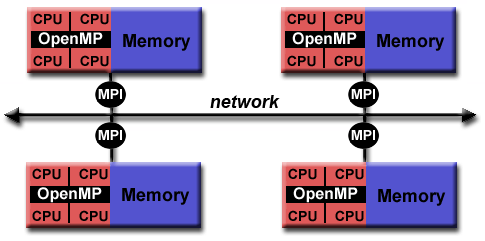
\includegraphics[scale=0.8]{./images/hybrid_model}
\caption{Hybrid memory architecture (Each processor is milti-core)}
\label{fig:hybridMemory}
\end{figure}

\item[Distributed Memory]
	Different systems, and hence, different processors connected via some
	kind of network (see figure \ref{fig:distribuiteMemory}) (usually high speed
	networks) and the memory space in one processor do not map to another processor. Each of them operate independently on its memory space,
	so changes are not reflected on memory spaces of the others. Explicit
	communication is required between processors and is like synchronization
	programmer's responsibility.
This architecture  is very scalable and there's not any overhead in maintaining
cache coherency but all the communication work rely on the programmer.

The most used paradigm for programming distributed memory machines is the
message passing\footnote{MPI is the \textit{de facto} industry standard for
message passing. Visit  \url{http://www.mpi-forum.org/}} for further
informations.

\item[Hybrid Systems] As the name suggest is a mix of the two architectures seen
before. Only a limited number of  processors, say N, have
access to a common pool of shared memory. These N processor are connected to the
others via network and each processor can consist of many cores.
A common example of a  programming model for hybrid system is the combination
of the message passing model (MPI) with the threads model (OpenMP) in which
\begin{inparaenum}[\itshape a\upshape)]
\item threads perform computationally intensive task, using local
\textbf{on-node} memory space and
\item communications between processes on different nodes occurs over network
using MPI (see figure\ref{fig:hybridMemory}).

\end{inparaenum} 
\end{description}


\begin{figure}
\centering
\setlength{\fboxrule}{0.5pt}%
\subfigure[UMA]{ \fbox{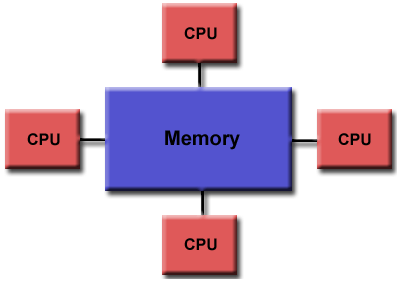
\includegraphics[scale=0.47]{./images/shared_mem}}}
\hfill
\subfigure[NUMA]{\fbox{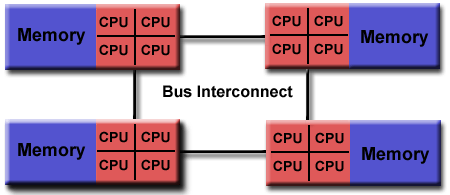
\includegraphics[scale=0.47]{./images/numa}}}
\hfill
\caption{Shared memory architectures.}
\label{fig:UMA_NUMA}
\end{figure}

\section{Network Topologies}
An important role is played, as seen before, by the interconnection network 
because provide mechanisms for data transfer between processing nodes.
Typically they consist of \textit{n} inputs and \textit{m} outputs and are built
in by switches and links (set of wires or fibers capable of carrying
information\footnote{Links may have different characteristics depending on
the material they are made of that can limit speed propagation of the signals
or the maximum length of the wire itself}).
\begin{figure}
\begin{center}
\caption{Start network topology}
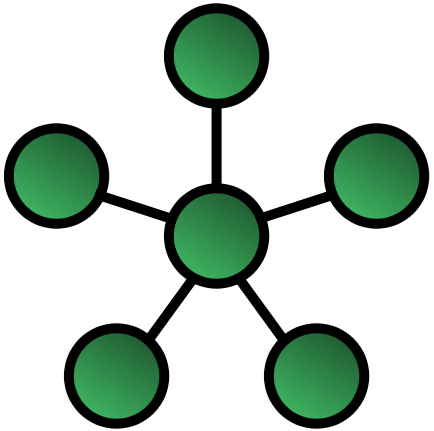
\includegraphics[scale=0.30]{./images/StartMesh}
\label{fig:starMesh}
\end{center}
\end{figure}
A first classification can be done considering only if the nodes are connected
directly to each others or not. In the first case the entire network consist of
point-to-point links and they are called \textbf{\textit{static}} or
\textbf{\textit{direct}} networks. On the other hand when the nodes are
connected to each others using switches we talk about \textbf{\textit{indirect}}
networks. Because communication is an important task in parallel computing,
the way the nodes are connected to each other is important and can influence
the overall performance of the system that is determined by the capabilities of
the network access devices, the level of control or fault tolerance desired, and
the cost associated with cabling or telecommunications circuits.
Networks topologies try to trade off cost and scalability with performance

\subsection{Bus-based networks}\label{bus-based}
The most simple family of topologies that give birth to the bus-based
networks. Each node is connected to a single shared medium that is common to all
the nodes. The most important advantage of bus is that the distance of two nodes is constant \textit{O}(1) and the cost scale linearly
as the number of nodes \textit{p}\footnote{The cost is usually associated with
the bus interface coupled with each node and is inexpensive to implement
compared to other topologies}.
A message from the source is broadcasted to all machines connected to the bus
and every machine ignore the message except for the intended address for the
message that accept the data. The low cost of implementing this topology if
tradeoff by the difficulties in managing it and plus, because of the bounded
bandwidth of buses, typical bus-based machine are limited to dozen of nodes.

\subsection{Completely connected networks}
In a completely-connected network, each node has a direct communication link to every other
node in the network. This kind of networks don't need any switching or
broadcasting mechanism because a node can send a message to another in a single
step, and interferences during the communication are completely prevented.
But completely connected network are not suitable for practical uses because of
the cost related to their implementation. The number of connection grows
quadratically \(O(p^2)\) with the number of the nodes (see figure
\ref{fig:completelyConnected}).
\[
c=\frac{n(n-1)}{2}
\]

\begin{figure}
\begin{center}
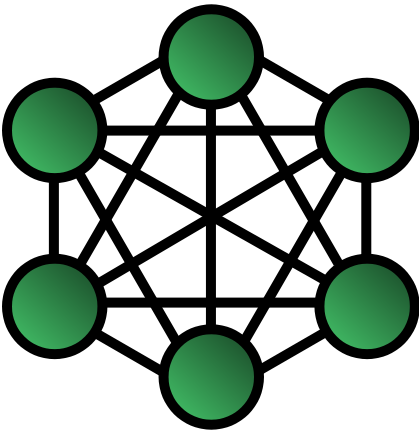
\includegraphics[scale=0.4]{./images/FullMesh}
\caption{Fully connected mesh network. 6 nodes and c=15 links}
\label{fig:completelyConnected}
\end{center}
\end{figure}



\subsection{Star-Connected Networks}

Star topology (see figure \ref{fig:starMesh}) every node is connected to
a central node that acts as the central processor (as server if we consider the
analogy with the LAN) . It is similar to the bus-based (see section \ref{bus-based}) network, because communication
between any pair of nodes is routed through the central processor (and the
latter is the shared medium the all the other nodes share) and because the
central processor is the bottleneck in this topology and also the single point
of failure (if this node goes down  the entire network stops to work).




\subsection{K-Meshes}


\begin{wrapfigure}{r}{0.4\textwidth}
\centering
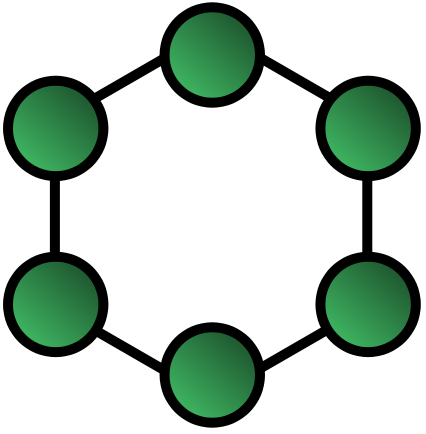
\includegraphics[scale=0.3]{./images/ring}
\caption{1-mesh ring topology}
\setlength{\fboxrule}{1pt}%
\label{fig:ring}
\end{wrapfigure}
Due to the large number of links in fully connected networks, sparser networks
are typically used to build parallel computers. A family of such networks spans the space of linear arrays and
hypercubes.
Linear array or ring are static network in which each node is connected with
other two (called neighbors, see figure \ref{fig:ring}).

The 2-D version of the ring topology is the 2-D torus (see figure
\ref{fig:torus}).
It consist of \(\sqrt{p}\) processor per each dimension, and each processor is connected to
four neighbors (ones whose indices differ in any dimension by one). 2-D or 3-D
meshes are very often used to build parallel machines because they are attractive from a
wiring standpoint (2-D mesh laid out in 2-D space) and because it naturally
maps a variety of computation ( matrices, 3-D weather modeling, structural
modeling, etc.). 



\begin{figure}
\caption{2D (a) and 3D (b) torus topologies.}
\label{fig:torus}
\centering
\setlength{\fboxrule}{0.5pt}%
\subfigure[2D]{ 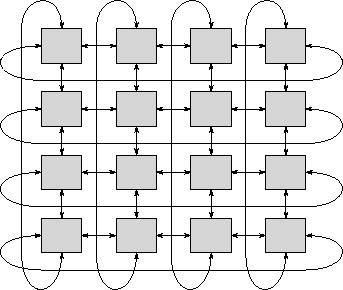
\includegraphics[scale=0.47]{./images/torus2D}}
\hfill
\subfigure[3D]{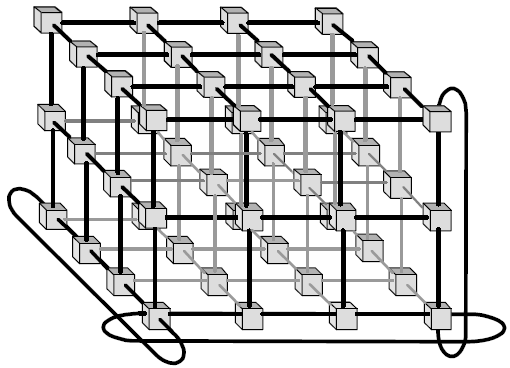
\includegraphics[scale=0.47]{./images/torus3D}}

\end{figure}

\subsection{Three based}
This type of network topology is based on a hierarchy of nodes. The highest
level of any tree network consists of a single node, the ``\textit{root}'' that
connects nodes (a fixed number referred to as the ``branching
factor''\footnote{If the branching factor is \(1\) the topology is called
linear.} of the tree) in the level below by point-to-point links. These lower
level nodes are also connected to nodes in the next level down. Tree networks
are not constrained to any number of levels, but as tree networks are a variant
of the bus network topology, they are prone to crippling network failures should
a connection in a higher level of nodes fail/suffer damage.
This topology exhibits good scalability and thanks to the different levels makes
fault identification and isolation easier but the maintenance may be an issue
when the network spans a great area.



%% This is an example first chapter.  You should put chapter/appendix that you
%% write into a separate file, and add a line \include{yourfilename} to
%% main.tex, where `yourfilename.tex' is the name of the chapter/appendix file.
%% You can process specific files by typing their names in at the
%% \files=
%% prompt when you run the file main.tex through LaTeX.
\lstdefinestyle{codeStyle}{
language=C++,
    basicstyle=\footnotesize\ttfamily,
    keywordstyle=\color{blue}\ttfamily,
	keywordstyle=[2]\color{darkgreen},
    stringstyle=\color{red}\ttfamily,
    commentstyle=\color{green}\ttfamily,
    columns=flexible,
    gobble=4,
    frame=L,
    numbers=left,
    numberstyle=\tiny,
	%belowcaptionskip=2em,
    %belowskip=5em,
}

\lstdefinestyle{codeStyleFramed}{
language=C++,
    basicstyle=\footnotesize\ttfamily,
    keywordstyle=\color{blue}\ttfamily,
	keywordstyle=[2]\color{darkgreen},
    stringstyle=\color{red}\ttfamily,
    commentstyle=\color{green}\ttfamily,
    columns=flexible,
    gobble=4,
    frame=single,
    numbers=left,
    numberstyle=\tiny,
%	belowcaptionskip=2em,
 %   belowskip=5em,
}


\chapter{GPGPU - History And Motivation}


\section{Introduction}
GPGPU, acronym for General-purpose computing on graphics processing units, is a
recent phenomenon wich consist in the utilization of a graphics processing unit
(GPU\footnote{Graphic processing unit, term conied by Nvidia in the
mid-nineties, and now the most common acronym used.}), which typically handles
computation only for computer graphics and was optimized for a small set of
graphic operation, to perform computation in applications traditionally handled
by the central processing unit (CPU). Those operations (generation of 3D images)
are intrinsically parallel, so, is not surprising if the underlying hardware has
evolved into a highly parallel, multithreaded, and many-core processor. The GPU excels at fine grained,
data-parallel workloads consisting of thousands of independent threads executing vertex,
geometry, and pixel-shader program threads concurrently.
Nowadays, the GPUs are not limited to its use as a graphics engine; there is a rapidly
growing interest in using these units as parallel computing architecture due to the tremendous
performance available in them. Currently, GPUs outperform CPUs on floating
point performance and memory bandwidth, both by a factor of roughly
100\cite{NvidiaprogGuide}, easily reaching computational powers in the
order of teraFLOPS. GPU works alongside the CPU providing an heterogeneous
computation, simply offloading compute-data-intensive portion of program on GPU
using it as co-processor highly specialized in parallel tasks.
Plus since 2006, date when Nvidia has introduced CUDA, is extremely simple to
program these kind of devices for general purpose tasks, although before that
date this goal was achieved dealing directly with the graphic API using shaders
with all the related constraints such as lack of integers or bit operations.



\section{Why GPU computing?}
Traditionally performance improvements in computer architecture have come from
cramming ever more functional units onto silicon, increasing clock speeds and
transistors number. Moores law\cite{mooreLaw1965} states that the number of
transistors that can be placed inexpensively on an integrated circuit will
double approximately every two years.
\begin{figure}
\centering
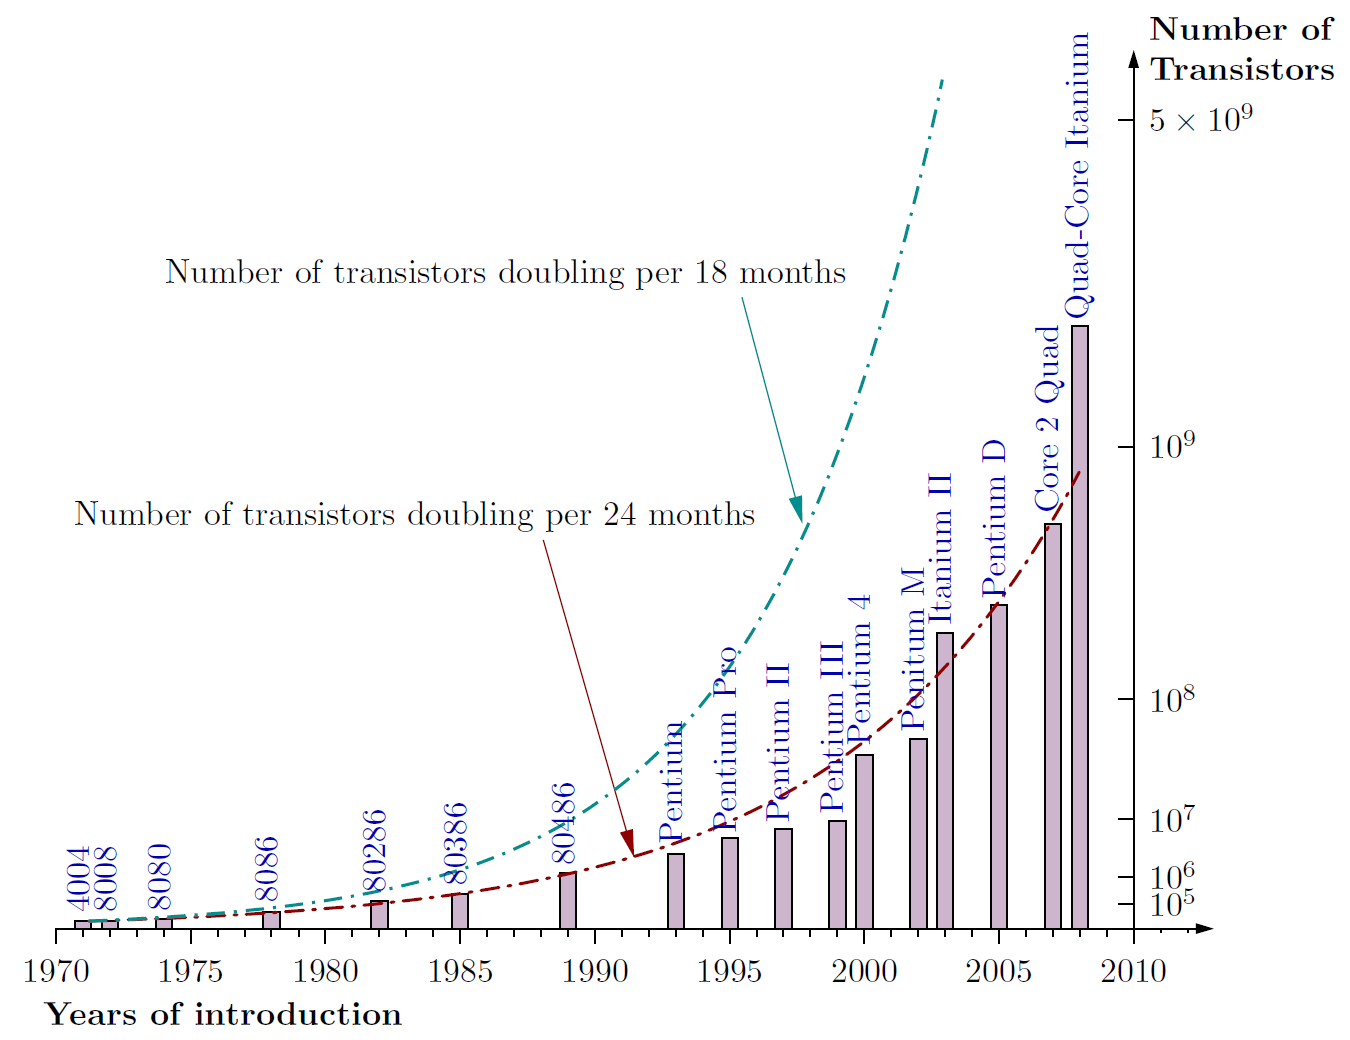
\includegraphics[totalheight=0.5\textheight]{./images/moore_law_large}
\caption{Moore's Law and intel family CPU transistors number
history.}\label{mooreLaw}
\end{figure}

Coupled with increasing clock speeds CPU performance has until recently scaled
likewise. But this trend cannot be sustained indefinitely or forever.
Increased clock speed and transistor number require more power and generate more
heat. Although the trend for transistor densities has continued to steadily increase,
clock speeds began slowing circa 2003 at 3 GHz. If we apply Moore's law type
thinking to clock-speed performance, we should be able to buy at least 10 GHz CPUs. However, the fastest CPU available today is 3.80 GHz 
At same point the performance increase fails to increase proportionally
with the added effort in terms of transistors or clock speed because efficient
heat dissipation and increasing transistor resolution on a wafer becomes more
important and challenging (there will be still the physical limit of dimension
for each transistor, the atom).
The heat emitted from the modern processor, measured in power
density	\begin{math}(\frac{W}{cm^2})\end{math} rivals
the heat of a nuclear reactor core\cite{Gelsinger2004}.
\begin{figure}[h!]
\centering
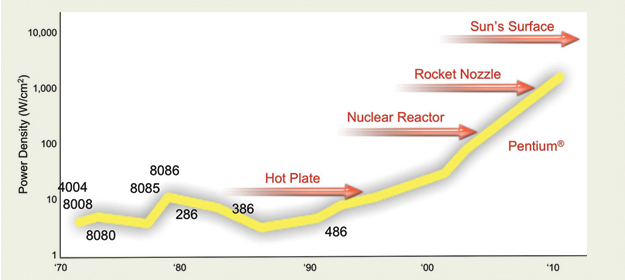
\includegraphics[scale=0.7]{./images/temperatureCPU}
\caption{Temperature CPUs}\label{tempCPU}
\end{figure}
But the power demand did not stop in these year, here the necessity of
switching on parallel architectures, so today the dominating trend in commodity CPU
architectures is multiple processing cores mounted on a single die operating at
reduced clock speeds and sharing some resources. Today is normal to use the so-called
multi-core (2,4,8,12) CPUs on a desktop PC at home.



\section{From Graphics to General Purpose Computing}
The concept of many processor working together in concert in not new in the
graphic field of the computer science. Since the demand generated by
entertainment started to growth multi-core hardware emerged in
order to take advantage of the high parallel task of generating 3D image.
In computer graphics, the process of generating a 3D images consist of
refreshing pixels at rate of sixty or more Hz. Each pixel to be processed
goes through a number of stages, and this process is commonly referred to as
the graphic processing pipeline. The peculiarity of this task is that the
computation each pixel is independent of the other's so this work is perfectly
suitable for distribution over parallel processing elements.
To support extremely fast processing of large graphics data sets (vertices and fragments), modern GPUs employ a
stream processing model with parallelism.
The game industry boosted the development of the GPU, that offer now greater
performance than CPUs and are improving faster too (see Figure
\ref{CPU-VS-GPU_GFLOP} and \ref{CPU-VS-GPU_MEMORY}).
The reason behind the discrepancy in floating-point capability between CPU and
GPU is that GPU is designed such that more transistors are devoted to data
processing rather than caching and flow control.

The today's Top 500 Supercomputers\footnote{\url{http://www.top500.org/statistics/list/}} ranking is
dominated by massively parallel computer, built on top of superfast networks and millions of
sequential CPUs working in concert but as the industry is developing even more
powerful, programmable and capable GPUs in term of GFlops  we see
that they begin to offer advantages over traditional cluster of computers in
terms of economicity and scalability.

\begin{figure}
\centering
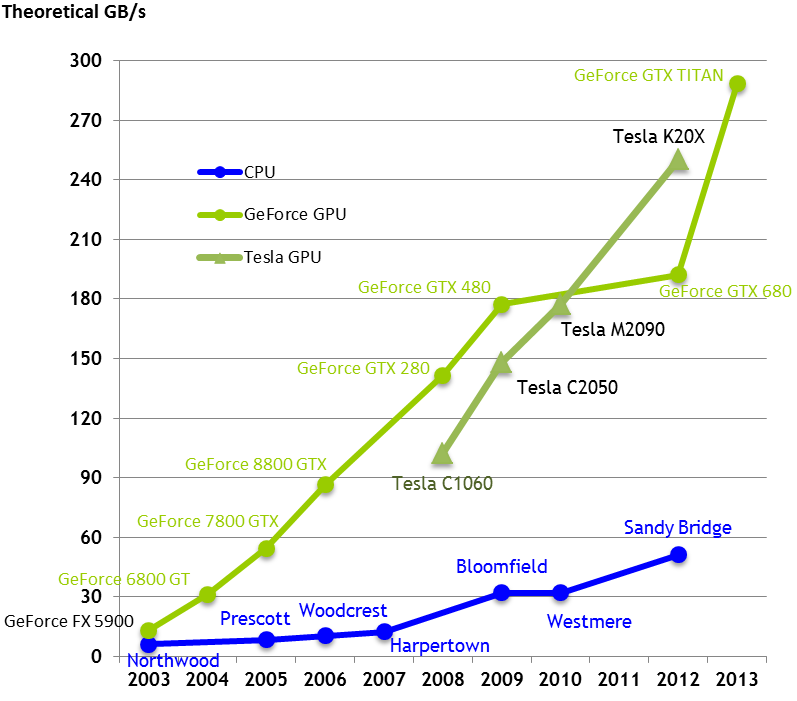
\includegraphics[scale=0.4]{./images/memory-bandwidth}
\caption{Intel CPUs and Nvidia GPUs memory bandwidth
chart}\label{CPU-VS-GPU_MEMORY}
\end{figure}
\begin{figure}
\centering
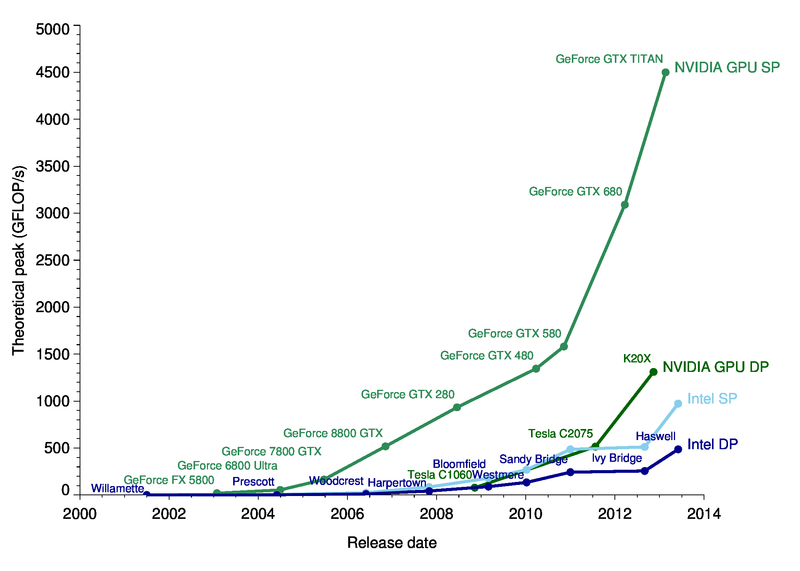
\includegraphics[scale=0.4]{./images/cpu-vs-gpu}
\caption[Intel CPUs and Nvidia GPUs Peak G/FLOPS chart]{Intel CPUs and Nvidia
GPUs (single and double precision) Peak G/FLOPS chart}\label{CPU-VS-GPU_GFLOP}
\end{figure}


\subsection{Traditional Graphics Pipeline}\label{graphicPipeline}
A graphics task such as rendering a 3D scene on the GPU
involves a sequence of processing stages (i.e. shaders) that run in parallel
and in a prefixed order, known as the graphics hardware
pipeline\footnote{http://duriansoftware.com/joe/An-intro-to-modern-OpenGL.-Chapter-1:-The-Graphics-Pipeline.html}
(see Figure \ref{graphicPipeline}).


The first stage of the pipeline is the vertex processing. The
input to this stage is a 3D polygonal mesh. The 3D world coordinates of each vertex of the mesh
are transformed to a 2D screen position. Color and texture
coordinates associated with each vertex are also evaluated.
In the second stage, the transformed vertices are grouped
into rendering primitives, such as triangles. Each primitive
is scan-converted, generating a set of fragments in screen
space. Each fragment stores the state information needed
to update a pixel. In the third stage, called the fragment processing, the texture coordinates of each fragment are used
to fetch colors of the appropriate texels (texture pixels) from
one or more textures. Mathematical operations may also be
performed to determine the ultimate color for the fragment.
Finally, various tests (e.g., depth and alpha) are conducted to
determine whether the fragment should be used to update a
pixel in the frame buffer.
Each shader in the pipeline performs a basic but specialised operation on the
vertices as it passes.
In a shader based architecture the individual shader processors exhibit very limited
capabilities beyond their specific purpose.
Before the advent of CUDA in 2006 most of the techniques for non-graphics
computation on the GPU took advantages of the programmable fragment processing
stage. The steps involved in mapping a computation on the GPU are
as follows:
\begin{figure}
\centering
\caption{Typical graphic pipeline}\label{graphicPipeline}
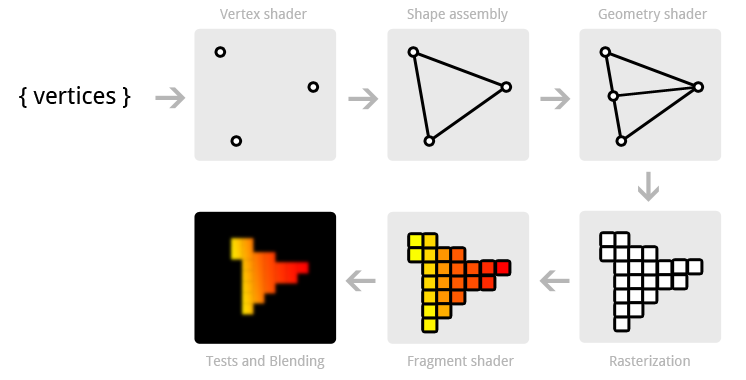
\includegraphics[scale=0.6]{./images/pipeline}
\end{figure}

\begin{enumerate}
	\item The data are laid out as texel colors in textures;
	\item  Each computation step is implemented with a
			user-defined fragment program. The results are encoded as pixel 
			colors and rendered into a pixel-buffer\footnote{ A buffer in GPU memory
			which is similar to a frame-buffer.}; 
	\item Results that are
			to be used in subsequent calculations are copied to textures for temporary
		storage.
\end{enumerate} 

The year 2006 marked a significant turning point in GPU architecture. The G80
was the first NVidia GPU to have a unified architecture whereby the different shader processors were
combined into unified stream processors. The resulting stream processors had to be
more complex so as to provide all of the functionality of the shader processors they
replaced. Although research had been carried out into general purpose programming
for GPUs previously, this architectural change opened the door to a far wider range of
applications and practitioners.
More in detail GPU are well-suited for problems highly data-parallel in wich the
same code is executed on many data elements at the same time (SIMD
paradigm\footnote{Single Instruction,
Multiple Data:
elements of short vectors are processed in parallel. To be clear CUDA paradigm is SIMT: Single
Instruction, Multiple Threads} or more generally as a CRCW PRAM
machine\footnote{Parallel random-access machine in which each thread can read
or write a memory cell.}).









\chapter{Compute Unified Device Architecture - CUDA }\label{chap:CUDA}
\section{Introduction}
\begin{wrapfigure}{I}{0.45\textwidth}

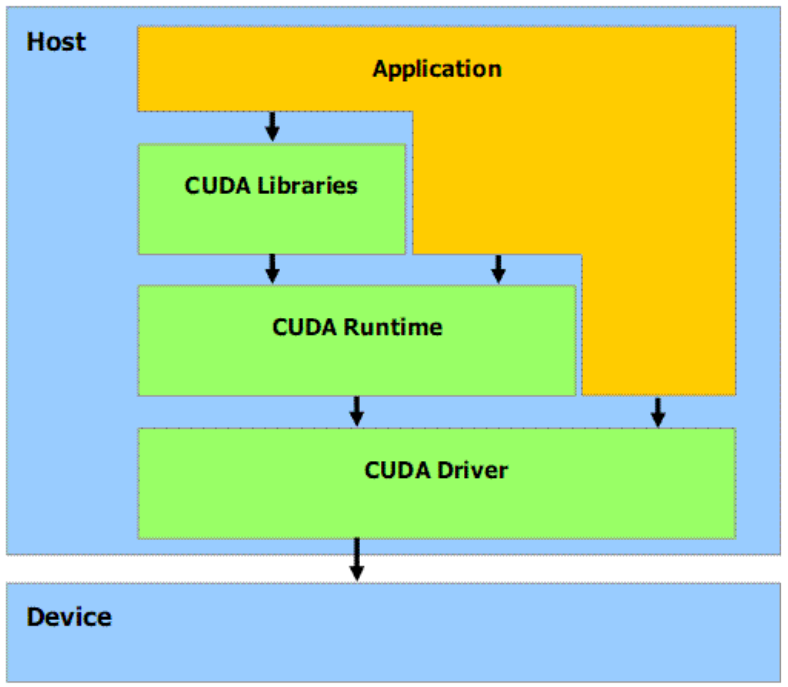
\includegraphics[scale=0.23]{./images/cudaArchitecture}
\caption{Cuda Software Stack}\label{CUDA_SOFT_ARCH}
\end{wrapfigure}
In November 2006 Nvidia released CUDA a platform (both hardware and software)
that allow the developers to use an high-level programming language
(e.g. C with slightly additions) to exploit the parallel power of the
hardware in order to solve complex computational problems in a more efficient
way than on a CPU. CUDA is attractive because is a complete system(software and
hardware model map well onto each other aiding the developer comprehension),
from silicon to high-level libraries and a growing experience exists providing a valuable resource to developers.
It is for these reason CUDA was selected as development platform for this work
rather than other platforms\footnote{e.g. OpenACC that proved to be
unsuitable to the parallelization of SCIARA-fv3}.
CUDA expose three level of components to an application (See figure
\ref{CUDA_SOFT_ARCH}):
\begin{enumerate}
\item \textit{\textbf{Cuda Driver}}:
	\begin{itemize}
	  \item Distinct from graphics driver. The only purpose of this component is to
	  provide the access to the GPU's general purpose functionalities.
	\end{itemize}
\item \textit{\textbf{CUDA Runtime}}:
	\begin{itemize}
	  \item Built on top of the CUDA Driver, provide an higher level of
	  abstraction making the code less cumbersome  especially as far as the
	  complexity of host code for kernel launches is concerned. 
	\end{itemize}
\item \textit{\textbf{CUDA Libraries}}:
 \begin{itemize}
	  \item Built on top of the CUDA Runtime, Is a collection of Libraries(CUBLAS,
	  CUSP, CUFFT, Thrust etc.)\footnote{For example CUFFT
	  provides an interface for computing Fast Fourier Transform
	  up to 10x faster than CPU
	  (\url{https://developer.nvidia.com/gpu-accelerated-libraries}).} providing full-suitable state of the art implementation of algorithms for a wide range of applications.
	\end{itemize}
\end{enumerate}


\FloatBarrier


\section{CUDA Hardware model}
There are various kind of CUDA capable device on the market. From a mid-level
laptop graphic card to a numerical computation dedicated
card.\footnote{For example GeForce GT 620M and Kepler K20x are respectively a
laptop and a dedicated numerical computation CUDA capable device.}
The Nvidia GPU hardware architecture is built around a scalable array of multithreaded \emph{Streaming Multiprocessors (SMs)}.
The \emph{Streaming Multiprocessors} is designed to execute hundreds of threads
concurrently  and contains a number of Streaming Processors (SP)\footnote{The SP
cores are also called \emph{CUDA cores} and the number of them depends on the
compute capability (See section \ref{computeCapability}) of the device. For
example v3.5 CUDA capability GPUs SM consists of 192 SPs. For v2.1
this number is 48, and for the old v1.x it is 8.}.





\subsection{Compute Capability}\label{computeCapability}
Each device comes with a revision number which defines the \emph{compute
capability} of the device, and it determines the set of features that can be
used for programming and the configuration in processors and memory.
The compute capability of a device is defined by a major revision number and a
minor revision number. Devices with the same major revision number are of the
same core architecture. The major revision number is 3 for devices based on the Kepler architecture, 
2 for devices based on the Fermi architecture, and 1 for devices based on the Tesla architecture.
The minor revision number corresponds to an incremental improvement to the core
architecture, possibly including new features\footnote{Here the table full
specification and features per Compute Capability:
\url{http://docs.nvidia.com/cuda/cuda-c-programming-guide/index.html\#compute-capabilities}}.
Furthermore, properties and features support can be queried using the runtime
API.
 Accelerators with capability 3.5, for example, were enhanced by dynamic
 parallelism(See section \ref{DynamicParallelism}).
 
 For this work we used as hardware test the Nvidia GeForce GTX 780 a GeForce GTX
680  respectively with compute capability 3.0 and 3.5 Kepler architecture and a
GeForce GTX 480 and GeForce GTX 580 both compute capability 2.0, Fermi
architecture.
For brevity purpose we are going to see in detail just the new Kepler
architecture.
\FloatBarrier
\subsection{Kepler Architecture}\label{sect:keplerArch}

NVIDIA Kepler architecture builds on the foundation first established in 2010 with NVIDIA's Fermi GPU
architecture.
The first GPU based on this new Kepler architecture, code-named ``GK104'' is
fabricated on a 28nm process, and every internal unit was designed for the best perf/watt possible. The
first product being introduced based on GK104 is the GeForce GTX 680.
Like Fermi, Kepler GPUs are composed of different configurations of Graphics
Processing Clusters (GPCs), Streaming Multiprocessors (SMs), and memory controllers.
The GeForce GTX 680 GPU consists of four GPCs, eight next-generation Streaming
Multiprocessors (SMX), and four memory controllers. In GeForce GTX 680, 
each GPC has a dedicated raster engine and two SMX units. With a total of eight
SMX units, the GeForce GTX 680 implementation has 1536 CUDA Cores (See figure
\ref{gtxArch} and table \ref{tab:cudaGtxspec}).
\begin{figure}
\centering
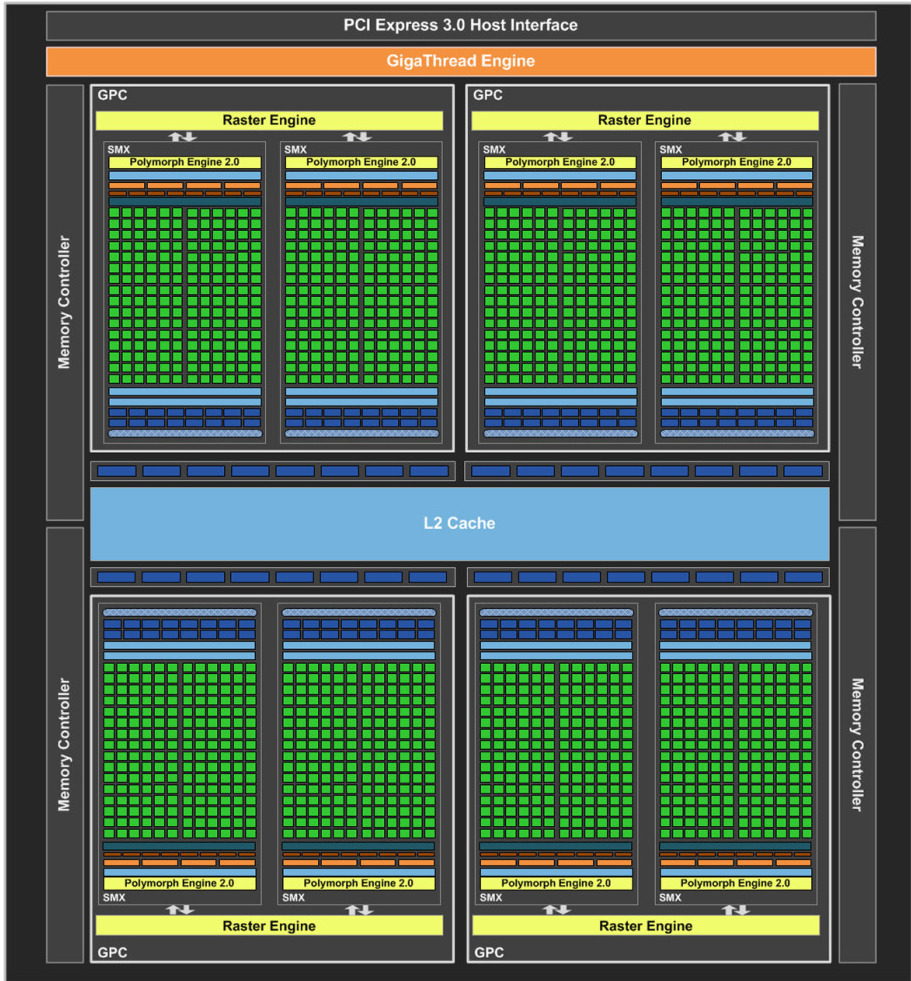
\includegraphics[scale=0.5]{./images/gtxArch}
\caption{Kepler Architecture (GTX 680)}\label{gtxArch}
\end{figure}
\FloatBarrier
Tied to each memory controller are 128KB L2. 
With four memory controllers, a full GeForce GTX 680 GPU has 512KB
L2 cache.

\begin{table}
	\centering
    \caption{High-level comparison of Kepler vs. Fermi GPUs}
\label{tab:cudaGtxspec}
\begin{tabular}{ | l | l | l |}
    \hline
    \textbf{\textit{GPU}} 		& \textbf{\textit{GTX 680}} &
    \textbf{\textit{GF110(Fermi)}}
    \\ \hline \textbf{\textit{Transistor}}  & 3.54 billion & 3.0    billion\\
    \hline \textbf{\textit{CUDA Cores}}  & 1536		  & 512\\ \hline
    \textbf{\textit{Graphic Core Clock}}  & 772 MHz & 1006 MHz  \\ \hline
    \textbf{\textit{GFLOPs}}  & 3090 & 1581\\ \hline
    \textbf{\textit{Memory Clock}}  & 6008 MHz & 4008 MHz\\ \hline
    \textbf{\textit{Memory Bandwidth}}  & 192.26 GB/sec & 192.4 GB/sec\\ \hline
    \textbf{\textit{TDP}}  & 195 W & 244 W\\ \hline
\end{tabular}   
\end{table}
    

\subsubsection{Streaming MultiProcessor-SMX}
The SM is the heart of NVIDIA unified GPU architecture. Most of the key
hardware units for graphics processing reside in the SM. The SM CUDA cores perform pixel/vertex/geometry shading and
physics/compute calculations. Texture units perform texture filtering and load/store units fetch and
save data to memory. Special Function Units (SFUs) handle transcendental and graphics interpolation
instructions. There are eight SMX in GeForce GTX 680 instead of sixteen as in
the GTX580).
\begin{wrapfigure}{r}{0.45\textwidth}
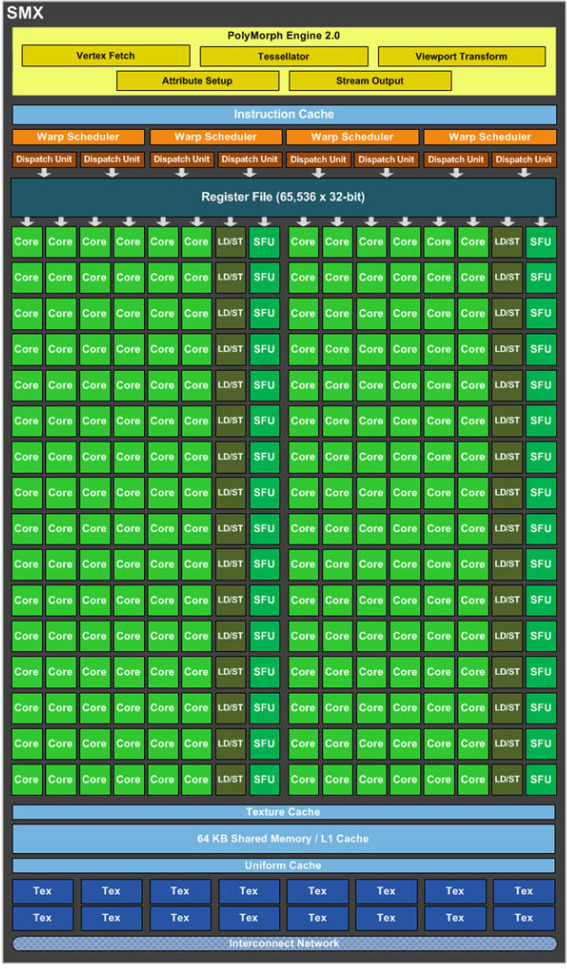
\includegraphics[scale=0.5]{./images/gtx680_SMX}
\caption{GTX 680 SMX Architecture Detail}\label{gtx680_SMX}
\end{wrapfigure}
To feed the execution resources of SMX, each unit contains four warp schedulers, and each warp
scheduler is capable of dispatching two instructions per warp every clock.
More importantly, the scheduling functions have been redesigned with a focus on power efficiency. For
example: Both Kepler and Fermi schedulers contain similar hardware units to handle scheduling
functions, including, (a) register score boarding for long latency operations (texture and load), (b) inter-
warp scheduling decisions (e.g., pick the best warp to go next among eligible candidates), and (c) thread
block level scheduling (e.g., the GigaThread engine);
The SMX schedules threads in groups of 32 parallel threads called warps. Each SMX features four warp 
schedulers and eight instruction dispatch units, allowing four warps to be issued and executed 
concurrently. Kepler's quad warp scheduler selects four warps, and two
independent instructions per warp can be dispatched each cycle. 
All cores in a multiprocessor have on-chip shared resources, including 255 local
32- bit registers per thread and one on-chip fast memory of size 64Kbyte, which
enable threads cooperation and transparent caching\footnote{it is possible to
use as user managed cache max of 48kb. There are two shared memory configuration
available per kernel. 16kb cache and 48kb user managed or viceversa.}.
Threads variables typically reside in live registers. The on-chip shared memory has
very low access latency and high bandwidth similar to an L1 cache; it holds CUDA variables
for the active thread blocks. The shared memory allows the parallel threads run on the cores in
a MP to share data without sending it over the system memory bus.




\FloatBarrier
\newpage
\section{CUDA Programming model}\label{cudaProgrammingModel}

CUDA programming model is designed to fully expose parallel capabilities of NVIDIA GPUs.
Even though the language is devoted to general purpose computing, it still requires the
programmer to follow a set of paradigms arising from the GPU architecture.
CUDA provides a few easily understood abstractions that allow the programmer to
focus on algorithmic efficiency and develop scalable parallel applications by expressing the
parallelism explicitly. It provides three key abstractions as hierarchy of
thread groups, shared memories, and synchronization barrier that provide a
clear parallel structure to conventional C code for one thread of the hierarchy.
\begin{wrapfigure}{l}{0.55\textwidth}
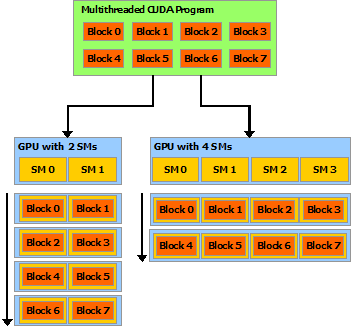
\includegraphics[scale=0.9]{./images/automatic-scalability}
\caption{Automatic Scalability}\label{automatic-scalability}
\end{wrapfigure}
\FloatBarrier
The abstractions guide the programmer to partition the
problem into coarse sub-problems that can be solved independently in parallel, and then into
finer pieces that can be solved cooperatively in parallel. The programming model scales
transparently to large numbers of processor cores: a compiled CUDA program executes on any
number of processors, and only the runtime system needs to know the physical
processor count (See figure \ref{automatic-scalability}).

\subsection{Host and Device}
CUDA paradigm is heterogeneous computation:
serial portions of applications are run on the CPU, and parallel portions are
off loaded to the GPU.
The CPU and GPU are treated as separate devices that both host and device
are equipped with their own memory spaces(referring to them, respectively as to
the host memory and device memory). This configuration also allows simultaneous and overlapped

\subsection{Kernels Functions And Thread Hierarchy}\label{kernels}
\begin{wrapfigure}{l}{0.540\textwidth}
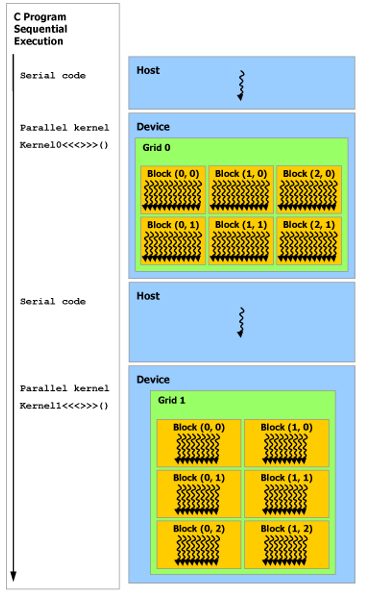
\includegraphics[scale=0.9]{./images/heterogeneous-programming}
\caption{Heterogeneous Programming}\label{heterogeneous-programming}
\end{wrapfigure}
Host code schedules kernels to be executed on the GPU, which also specifies
starting configuration of the kernel.
Kernel code is compiled by nvcc the Nvidia CUDA compiler and sequential code by
the host's normal C\footnote{For example GCC on Unix or Visual C++ on Windows
systems.} compiler which is then linked to create a single binary executable.
A kernel can be ``launched'' using thousands
or even millions of “lightweight� threads that are to be run on the device.
computation on both the CPU and GPU without contention for memory resources (See figure \ref{heterogeneous-programming}).
The programmer is encouraged to “think big� and schedule threads liberally and
as needed. Cuda threads are thought as lightweighted for these because there
is not any creation overhead and can be created quickly, scheduling of blocks
and threads is handled directly on hardware avoiding any software overhead. 
More threads can hide latency caused by data fetching, leading to performance gains.
A kernel is an extension to the standard C function that are executed N times
by different N threads(as opposed to only one like regular C function).
 kernel is defined specifying the \textbf{\color{green} \_\_global\_\_} keyword
and the \textit{execution configuration}
\textless\textless\textless \ldots \textgreater\textgreater\textgreater. Each
thread is given a unique \textit{threadID} that is accessible through the
built-in variable(a 3-component C-structure) threadIdx. (See listing
\ref{code:kernelInvocation} at page \pageref{code:kernelInvocation}).

The threads are organized by the programmer by defining a grid and making a division
of the grid in thread blocks or just blocks, (see figure \ref{threadHierarchy}
and \ref{kernelGrid}).
The index of the blocks and threads in x, y and z direction can be retrieved
,within a kernel, via statements like: by = blockIdx.y, and tz = threadIdx.z (as
well as the grid dimension via dimGrid.(x,y,z)).
We can assign a unique (for the grid) global ID to each thread by combining
both thread and block index, e.g. for a 2D grid and 2D block \(threadIDx = blockDim.x
\times blockIdx.x + threadIdx.x \) and \(threadIDy = blockDim.y \times blockIdx.y +
threadIdx.y\). It is useful when we want to assign a portion of work to each
thread and divide the work among them\footnote{E.g. In a parallel matrix
summation algorithm we can assign a unique pair of matrix's cells to be summed
to each thread, and them could retrieve the correct pair just using their global
ID.}
\begin{center}
\begin{figure}
\centering
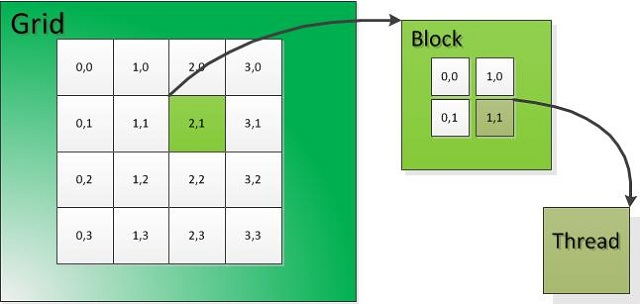
\includegraphics[scale=0.8]{./images/thread_hierarchy1}
\caption{The CUDA architecture on a conceptual level. The grid is divided into blocks that each consists of a number
of threads.}
\label{threadHierarchy}
\end{figure}
\end{center}
\FloatBarrier

Each block consists of a batch of threads, and can be a 1D, 2D or 3D object.
This provide a natural and intuitive way to compute on data structure like
array(1D), matrix(2D) or volume(3D).
\begin{figure}
\centering
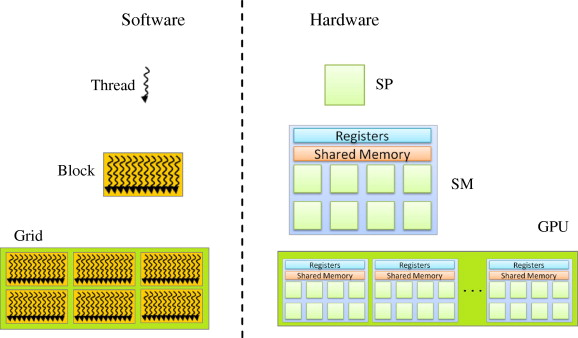
\includegraphics[scale=1.1]{./images/mappingSofthard}
\caption{Mapping Hardware-Software}\label{mappingSofthard}
\end{figure}

\begin{wrapfigure}{r}{0.62\textwidth}
\caption{Kernels Grid}\label{kernelGrid}
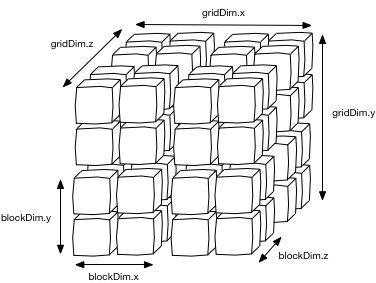
\includegraphics[scale=0.66]{./images/cuda-grid}
\end{wrapfigure}
The maximal number of threads per block and
the maximum dimensionality of the grid and the block which is allowed depends on
the compute capability (section \ref{computeCapability})and that limit exist because all threads of a
block reside on the same multiprocessor and they share its resources as
shared/registers memory or cores. On GTX 680 the maximum number of thread per
block is 1024 and the maximum sizes of each dimension of a block is \begin{math}1024 \times 1024 \times 64\end{math}.

It means that, the dimensionally of a
block launched on a GTX 680 must satisfy:
\[
\begin{cases} 

			xBlockDim \times yBlockDim \times zBlockDim=1024 \\
			 1\le xBlockDim \le 1024 \\
			  1\le yBlockDim \le 1024 \\
			  1\le zBlockDim \le 64\\  
\end{cases}
\]
Plus a kernel can be launched and executed only by equally shaped kernel so the
total number of threads is the number of threads per block times the number of blocks\footnote{Blocks of
\(32\times32\) threads are allowed as well as \(16\times16\times2\). Blocks of
\(2\times2\times128=512\) threads are not allowed because zDim is greater than zDim's limit(64).
\(16\times16\times16=4096\) is not allowed because 4096 is greater than the maximum
permitted number of thread per block.}.
The blocks are divided amongst the physical processors of the GPU, and threads
inside a block are grouped in warps.
A warp consist typically of 32 threads with consecutive indices that are in
principle having their instructions executed simultaneously on the
multiprocessor\footnote{The scheduler(one or more per SM) select threads for
execution in granularity of warps. Hence the name of \emph{warp
scheduler}.}(SIMD).
If one or several threads executes conditional code that differ in code path
from other threads in the warp (SIMT), these different execution paths are
effectively serialized, as the threads need to wait for each other. This
phenomenon is referred to as \emph{thread divergence}\label{threadDivergence}
\footnote{A common situation that cause divergence involves branch condition
that are function of the thread id and the branch granularity is not a whole
multiple of the warp size, and so not all the threads in the same warp follow the same path.
E.g.: \(if (threadIdx.x \ge 5)\) is divergent code instead of 
\(if (threadIdx.x / WARP\_SIZE > 2)\) that avoid divergence unless it has a
branch condition dependent on thread id.
}, a situation that should be avoided as much as possible.
Threads inside a block can cooperate by communicating and sharing (see section
\ref{shareMemory}) data through shared memory or by synchronizing their
execution via the \textbf{\_\_syncthreads()} intrinsic function that acts as barrier at block
level. 

\subsection{Memory model}\label{memoryModel}


Different kind of memories can be accessed by threads during their execution,
and can be classified regarding their degree of privacy and their speed (See
table \ref{tab:memoryHierarchyScope}).
All threads have free access to \emph{global memory} or also called \emph{device
memory}. Threads within the same block have access to so called \emph{shared
memory} that can be used for cooperation between thread of the same block and,
at the end, each thread has his own local and private \emph{registers}. There
are other two memory spaces that can be addressed by all threads: constant and
texture memories each specialized for different usage, but the shared
characteristic is that they are persistent across kernels launch\footnote{Within
the same application.}.



\subsubsection{Device Memory}
\begin{wrapfigure}{r}{0.5\textwidth}
\caption{Memory Hierarchy}\label{memoryHierarchy}
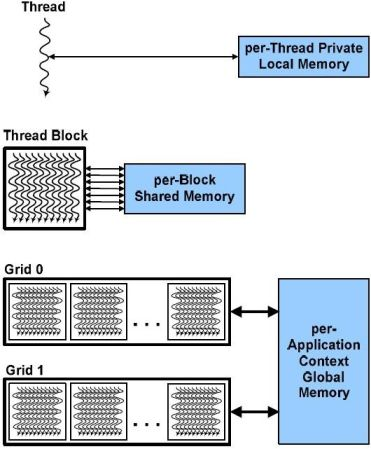
\includegraphics[scale=0.9]{./images/memoryhierarchy}
\end{wrapfigure}

The most prominent feature of device memory is its high capacity,
up to 6GB (Tesla C2070), but is also slow (400 - 600 cycles
latency)\footnote{New devices are equipped with L2 cache (in Kepler 1.5MB), that
helps to mitigate this problem serving either load and write operations.}
prohibiting an extensive usage, when high performance is requested.
Parts of the DRAM are dedicated to constant memory and texture memory.

\subsubsection{Global Memory}
The most general space allowing both, reading and writing of data, is
the global memory. It is allocated and is allocated and managed 
by the host. Due to DRAM bandwidth optimizations and the GPU architecture, and, 
as each multiprocessor works independently, unordered reads and writes are
possible because all threads are able to read from all memory spaces at any
time without any mutual exclusivity mechanism. Is up to the programmer to avoid
race-conditions and incoherences.

An important concept related to the global memory that has to be kept in mind
when writing CUDA C code due to its performance consequence, it's the
memory coalescence.

 \hfill \\ \hfill \\
 \begin{table}
\caption{Memory architecture summary.}
 \label{tab:memoryHierarchyScope}
\begin{tabular}[l]{|l|l|l|l|l|l|}
\hline 
\textbf{Memory} & \textbf{Location}&  \textbf{Chached}& \textbf{Access} &
\textbf{Scope} & \textbf{LifeTime}\\ \hline \hline

\textit{Register} & On-Chip	 & N\textbackslash A	& R\textbackslash W & One
Thread & Thread\\
\hline \textit{Local} & Off-Chip & NO	& R\textbackslash W & One Thread & 
Thread\\ \hline \textit{Shared} & On-Chip  & N\textbackslash A & R\textbackslash W & All
Threads in a block & Block\\
\hline \textit{Global} & Off-Chip & NO 	& R\textbackslash W & All Threads +
Host & Application	\\
\hline \textit{Constant} & Off-Chip & YES  & R & All Threads + Host & 
Application\\
\hline \textit{Texture} & Off-Chip & YES  & R & All Threads + Host &
Application \\
\hline
\end{tabular}
\end{table}
\subsubsection{Coalescence}
Coalescence is the capability of the device of grouping global memory accesses
of threads whithin a warp.
Global memory loads and stores by threads of a warp \footnote{Half warp for
devices of compute capability 1.x)} are coalesced by the device into as few as
one transaction when certain access requirements are met.
Remanding that c.c. 3.5 global memory is only L2 cached, while for devices with
c.c. 2.x the concurrent accesses of the threads of a warp will coalesce into a
number of transactions equal to the number of cache lines necessary to service
all of the threads of the warp. By default, all accesses are cached through L1,
which has 128-byte lines. For scattered access patterns, to reduce overfetch, it
can sometimes be useful to cache only in L2, which caches shorter 32-byte
segments

In order to achieve coalescence there should be some
coherence\footnote{Depending on Compute capability, access requirements are
different and usually less constrained with newer devices.} in memory access by
adjacent threads running on the device.
Certain memory access patterns enable the hardware to coalesce groups of reads
or writes of multiple data items into one operation. Data that cannot be laid
out so as to enable coalescing (in general case) and, application that do not
exploit this feature will tend to see lesser speedups when used in computations
on CUDA.
Assuming compute capability 2.x the very first pattern that enable coalescence
is when the \(k-th\) accesses the \(k-th\) word in a cache line\footnote{128B
aligned memory} (not all threads need to partecipate).
Morever if the same scenario of sequential access happens, but on misaligned
with the cache line, two 128B loads are required in order to fill the L1 cache
or even more if L2 is used (see figure \ref{fig:misaligedCoalescence}, in red
loaded memory portions).
\begin{figure}
\centering
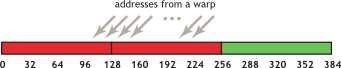
\includegraphics[scale=1.0]{./images/unaligned-sequential-addresses}
\caption{Parent Child Synchronization.}\label{fig:misaligedCoalescence}
\end{figure}


 
\subsubsection{Texture Memory}
As its name suggests, texture memory is used for storing textures.
Although this memory was designed for the classical openGL and DirectX graphic
pipeline (see section \ref{graphicPipeline}) it can be used successfully in some scenario to
accelerate the application especially when the memory access pattern exhibit
2D-spatial \footnote{A texture has
2-dimensions, so it's not surprising if this kind of memory is optimized
for 2D accesses.} locality it will give higher memory bandwidth by reducing requests to
the off-chip DRAM. Threads of the same warp that read texture addresses that are
close together, will achieve better performance using the texture
cache\cite{NvidiaprogGuide}. 

\subsubsection{Constant Memory}\label{sect:constantmemory}
Specific part of device memory is the constant memory, which allows to store limited
amount (64KB) of constant symbols. Similarly to the texture memory, the accesses
are cached but only reading is allowed. Constant memory should be used for small
variables that are shared among all threads and do no require interpolation.
It is declared by the host using the keyword \textbf{\_\_constant\_\_}, and its
size is to be known at compile time. There are two main reason why reading from
constant memory can save bandwidth:

\begin{itemize}\itemsep1pt
  \item A single read can be broadcasted to all thread of the same \emph{warp}.
  \item Constant memory is cached, so consecutive reads of the same address will
  not incur any additional traffic on off-chip DRAM.
\end{itemize}

\subsubsection{Shared Memory}\label{shareMemory}
Present on each SM. On the Fermi architecture card, there is 64KB of level 1
cache made up of SRAM. SRAM, or static random-access memory, is an expensive type of RAM, that
is much faster than DRAM. This cache is divided into two parts: a normal cache and a user managed
cache called the shared memory\cite{NvidiaprogGuide}. Depending on the program,
the L1 cache can be set to either be 16 or 48 KB, where the size of shared memory is the remainder.
As programmer the keyword \textbf{\_\_constant\_\_} make a variable resident
into shared memory. Cuda will create a copy of each variable for each block.
Each thread within a block share the \emph{shared memory}, and so, can modify or
read whichever address, but it cannot access to any other block's copy.
This provide an excellent mechanism by which threads can communicate and cooperate
on computations. It is a on-chip SRAM\footnote{Static random-access memory, more
expensive and less dense than DRAM.} and is very fast compared to the \emph{global
memory} (30-50 cycles latency) but it is only alive during the kernel call.
More in detail, shared memory is divided into multiple banks\footnote{That
number is fixed and depends on cc of the device; 16 on 1.x and 32 on 2.x for
instance.} (similar to banks in DRAM modules). Each bank can service only one
request at a time\footnote{Except when all thread within a warp access the
same address. In that case a broadcast operation is performed with no
performance decrease or superfluous memory accesses.}.
Shared memory banks are organized such that successive 32-bit words are assigned to successive banks and each bank has a bandwidth of 32 bits
per clock cycle. Therefore, any memory load or store of n addresses that spans n
distinct memory banks can be serviced simultaneously, yielding an effective
bandwidth that is n times as high as the bandwidth of a single bank but if
multiple addresses of a memory request map to the same memory bank, the accesses
are serialized\footnote{Situation knows as bank conflict.
http://cuda-programming.blogspot.co.uk/2013/02/bank-conflicts-in-shared-memory-in-cuda.html}.


\subsubsection{Registers}
\begin{wrapfigure}{r}{0.45\textwidth}
\caption{Kernel Grid}\label{dynamicParallelismSynch}
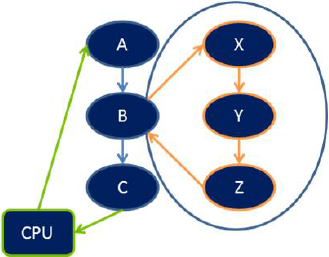
\includegraphics[scale=0.8]{./images/dynamicParallelismSynch}
\end{wrapfigure}
The registers on the GPU are general purpose. Each SM has a number of registers to share
between its cores. If too much register space is used by a kernel, the number of cores per SM that can
be utilized is lowered or local memory\footnote{A portion of device memory
devoted to the storage of local private per thread variables that do not fit
into registers.} can be utilized.
The Geforce GTX 480 has 32.768, 32-bit registers on each of the 15 SMs\footnote{It means 63
32-bit variable per thread for device with cc2.x and 3.0, but that number was
increased to 255 in cc 3.5.} and that memory is 8x faster\footnote{On
Fermi architecture, Volkov http://www.cs.berkeley.edu/~volkov/volkov10-GTC.pdf.
In device with cc 1.x that gap was not so big.} even than the already very
fast shared memory.



\subsection{Dynamic Parallelism}\label{DynamicParallelism}
Cuda 5.0 introduces a new feature,\emph{Dynamic
Parallelism}\cite{dynamicParallelism}\footnote{Only supported by devices with
compute capability 3.5 and higher.} that enable  CUDA kernel to create new work, using the API to launch new kernel,
perform device memory management, or library call (CUBLAS for instance) all
without CPU involvement (see example code \ref{code:dynamicParallelism} at page
\pageref{code:dynamicParallelism}).
This effectively eliminates the superfluous back and forth communication between the GPU and CPU through nested kernel computations.
The launching kernel is called the ``parent'', and the new grid it launches the
``child''.
Child kernels may themselves launch work, creating a nested execution
hierarchy\footnote{To a depth of 24 on Kepler architecture.} and giving the
possibility to easily exploit and port parallel nested algorithms or other
constructs that do not fit a flat, single-level of parallelism.
To be considered complete, a parent kernel all child grids created by its
threads(whichever it is within the kernel) have completed, even if the
programmer does not explicitly synchronize the threads the runtime guarantee
synchronization between parent and all the childs ( see figure
\ref{dynamicparallelismParentChild} and \ref{dynamicParallelismSynch}).
In the example in figure \ref{dynamicParallelismSynch} the kernel C will not be
able to begin execution until kernel Z has completed, because from
the point of view of C, kernels X,Y,Z are seen as part of B.
\begin{figure}
\centering
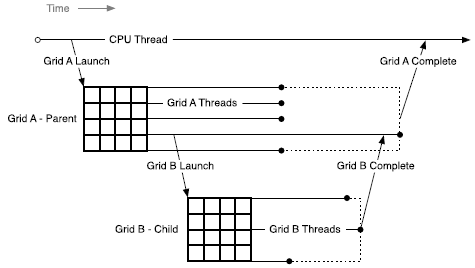
\includegraphics[scale=1.0]{./images/dynamicparallelismParentChild}
\caption{Parent Child Synchronization.}\label{dynamicparallelismParentChild}
\end{figure}
\FloatBarrier 
The same kind of coordination and synchronization holds between X,Y,Z, hence Y
can't begin the execution until X has returned. This allow the program flow can be handled ``on
GPU'' within one single kernel without any memory exchange between GPU and CPU, and also allow hierarchical call to be
written where data from a parent kernel is used to decide how to partition the
next lower level of the hierarchy (see figure
\ref{dynamicparallelismParentChild}) .

Consistency of global memory access is not guarantees between child and parent,
because as usual launches are asynchronous and it means that when a child grid
is invoked it return immediately the control to the parent kernel, and the
parent does not know when child is really executed.
So it can not rely on any assumption about the concurrent execution of the
child. There are just two point in the execution of a child grid when the memory
is fully consistent with the parent:
\begin{itemize}
  \item when a child is invoked.
  \item when the launching thread reaches a synchronization point.
\end{itemize}

Moreover childs and parent grid share the same global and constant memory, but
as kernels, have different and private local registers and shared memory.
It's illegal to use a pointer to local or shared memory as an argument to a
kernel launch.

\begin{figure}
\centering
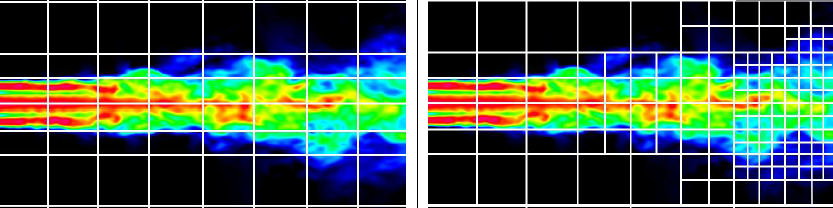
\includegraphics[scale=0.7]{./images/dynamicpParallelismWorkload.png}
\caption{An example of how the parent grid can launch
child grid with dynamic dimension to obtain a better
workload.}\label{dynamicpParallelismWorkload.png}
\end{figure}






\FloatBarrier


\subsection{Performance Guidelines}\label{sect:cudaPerfGuideline}
In this section we discuss some basic, frequently used technique to fully exploit
the computational power of the CUDA platform, but basically they revolve around
these concepts:
\begin{itemize}
  \item Maximize parallel execution to achieve maximum utilization;
 \item  Optimize memory usage to achieve maximum memory throughput;
 \item Optimize instruction usage to achieve maximum instruction throughput.
\end{itemize}


\subsubsection{Maximize Utilization}
At application level the programmer should maximize the device utilization by
using asynchronous function calls and streams\footnote{A CUDA stream is a
sequence of operation that execute in issue order on GPU.}.Different operations
in different streams can run concurrently giving (even if the device support
these kind of operation) better overall performance. At an high level of
abstraction we can think t streams as independent task that could, in theory,
run in parallel without any consequence on each other. At a lower level, the
application should maximize the occupancy. Nvidia provide with its SDK
a spreadsheet that enable the programmer to calculate those metrics\footnote{It can
be found here:
\url{http://developer.download.nvidia.com/compute/cuda/CUDA\_Occupancy_calculator.xls}}
However, maximize the occupancy is not a trivial task, because it can be
influenced by lot of factors and such kernel launch configuration settings,
number of registers utilized by threads or amount of shared memory utilized per block and compute capability.
Another important issue can be represented by the lower utilization of the
functional units. At every instruction issue time, a warp scheduler selects a
warp that is ready to execute its next instruction, if any, and issues the
instruction to the active threads of the warp. The number of clock cycles it
takes for a warp to be ready to execute its next instruction is called the
latency, and full utilization is achieved when all warp schedulers always have
some instruction to issue for some warp at every clock cycle during that latency
period, or in other words, when latency is completely "hidden".
The most common reason a warp is not ready to execute its next instruction is
that the instruction's input operands are not available yet.
For instance if some input operand resides in off-chip memory, the latency is
:400 to 800 clock cycles for devices of  compute capability 1.x and 2.x and
about 200 to 400 clock cycles for devices of compute capability 3.x, that is
much higher than registers's latency which is caused by register dependencies,
i.e. some of them are waiting for some previous instructions to be completed.
Synchronization is another source of latency, because warps waiting at some
synchronizing fence cannot be scheduled.
However is not possible to predeterminate the performance given only a execution
configuration. Experimentation is recommended to find out the best configuration
for the application. Obviously the number of threads per block should be chosen
of multiple of the warps size (i.e. 32) otherwise CUDA automatically pad
the resulting of blocks subdivision warps with \emph{fake} threads, wasting
resources.

\subsubsection{Memory throughput Utilization}
Memory transfer should be avoided, but some of them are
unavoidable especially if they are performed in low bandwidth. For instance
host to/from device bandwidth is much lower than device to device one.
One way to minimize data transfer between the host and the device is to move
more code from the host to the device, even if that means running kernels with
low parallelism computations and try to batch many small transfers into a single
large one, that always perform better.

\subsubsection{Memory throughput Utilization}

Shared memory and caches (i.e., L1/L2 caches available on devices compute
capability 2.x and higher) should be used to minimized memory transfers and
global memory accesses. The typical patter of a program that use shared memory
is :
\begin{itemize}%{labelitemi}{$\Rightarrow$}[leftmargin=1em]
  \renewcommand{\labelitemi}{$\diamondsuit$}
  \item Load data in shared memory. Usually each thread in a block load its
  address.
  \item Synchronize with the other threads so the memory is coherent after its
  population.
  \item Process data in shared memory as much as possible.
  \item Write back to device memory.
\end{itemize}
As explained in section \ref{memoryModel} accesses pattern is important even in
shared memory, so a second phase of optimization is often necessary to organize
accesses in order to enable coalesced access in case of global
memory\footnote{This pattern is more important because the non-optimal global
memory accesses have a higher impact on performance.} or avoid bank conflict
in shared memory.
\subsubsection{Optimize instruction throughput}
Use as much as possible intrinsic\footnote{Less accurate but faster function
directly mapped to fewer with native instruction. They are prefixed with
\emph{\_\_}. The compiler provide an option (\emph{-use-fast\_math}) that
convert automatically each function to an intrinsic one, obviously only those for which an equivalent
intrinsic exist. } function, avoiding function with low throughput and
prefer single precision instead of double precision\footnote{Only when precision
does not affect the end of the result. As we will se in this work, precision is very important.}.
Moreover programmer should be try to minimize thread divergence (see section
\ref{threadDivergence}) in order to not increase the total number of
instruction scheduled for a warp.
There are many other option that can permit a fine-tuning of the application
regarding integer and floating point arithmetics. But those techniques are not
crucial for the performance of the application unless they can give
back a good improvement in some scenarios.\footnote{For a full list of this
operations see CUDA programming guide
:\url{http://docs.nvidia.com/cuda/cuda-c-programming-guide/index.html\#maximize-instruction-throughput}}



\subsubsection{Library usage}
Cuda provide a large yes implemented state of the art functions that span from
linear algebra to AI algorithms\footnote{For the
complete list :https://developer.nvidia.com/technologies/Libraries.}.
Using them instead of writing own kernels one can accelerate the application
development and taking advantage of the performance gain given by the new version of the library due to redesigning of the algorithms or the exploitation of the latest GPU features.
For this work for instance we used Thrust that is a library of parallel
algorithms(sort, scan, transform, reduction etc.) and data structure (see
example code \ref{code:Thrust} at page \pageref{code:Thrust}).



\begin{figure}
\centering
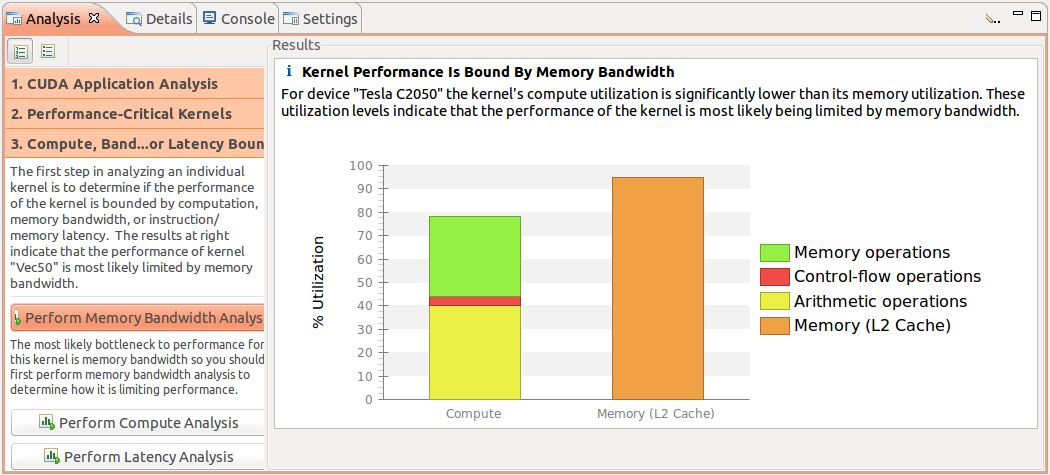
\includegraphics[scale=0.4]{./images/analysis-view.png}
\caption{Example of analysis of a kernel. The profiler gives
lots of metrics that are very useful to perform performance
tuning of the application and to identify bottleneck. In this
case the kernel is very memory bounded.}\label{profiler}
\end{figure}
\subsection{Nvidia Visual Profiler}

The NVIDIA Visual Profiler is a cross-platform performance profiling tool that
delivers developers feedback for optimizing CUDA C/C++ applications, identify
potential performance bottleneck issues and plus it provides optimization suggestions.
These informations are organized in tables that show activity occurring on both
CPU and GPU in a unified time line, including CUDA API calls, memory transfers
and CUDA kernel launches and each information is coupled with many other
statistics and metrics, like timing or occupancy.
This tools has access to the low level metric collected directly from the
hardware and low-level software instrumentation, like power, thermal or clock
situation of the devices.
See figure \ref{profiler} for an example of the kind of suggestions given by
this tools.

\lstdefinestyle{codeStyleC}{
language=C++,
basicstyle=\ttfamily\normalsize{},
keywordstyle=\color{blue}\ttfamily,
stringstyle=\color{red}\ttfamily,
commentstyle=\color{green}\ttfamily,
breaklines=true,
columns=flexible,
gobble=4,
xleftmargin=\leftmargini,
frame=L,
numbers=left,
numberstyle=\tiny,
belowcaptionskip=0.5em,
belowskip=1em,
}


\chapter{Alternatives to CUDA}
\section{Introduction}
The purpose of this section is to give an overall descriptions and introduction
of the alternative to CUDA. For this work we investigated more in
detail OpenCL and OpenACC. For a full description of all the platform
described here refers to the official documentation.


\section{OpenCL}
Released on December 2008 by the Kronos Group\footnote{A standards
consortium.} OpenCL is an open standard for programming heterogeneous computers
built from CPUs, GPUs and other processors that includes a framework to define
the platform in terms of a host, one or more compute devices, and a
C-based programming language for writing programs for the compute devices (see
figure \ref{openCL}).
One of the first advantages of OpenCL is that it is not restricted to the use of
GPUs but it take each resource in the system as computational peer unit,  easing
the programmer by interfacing with them. Another big advantage is that it is
open and free standard and it permit cross-vendor portability\footnote{One
of the most important supporter of OpenCL is ATI}.
\subsection{Model Architecture}
The model architecture follows that one already studied for
CUDA (see section \ref{cudaProgrammingModel}) but with different names.
\begin{figure}
\centering
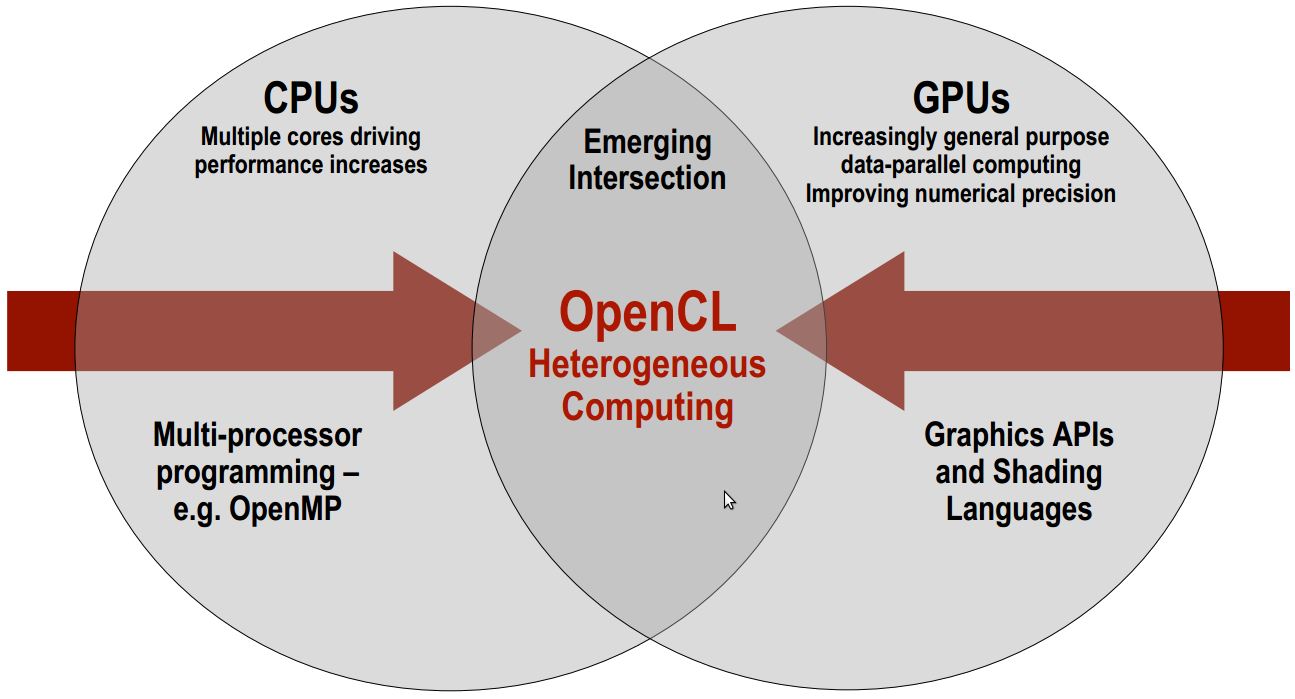
\includegraphics[scale=0.35]{./images/openCL1}
\caption{OpenCL heterogeneous computing.}\label{openCL}
\end{figure}



\begin{description}
  \item [Work-items:] \hfill\\ are equivalent to the CUDA threads and are the smallest execution
entity of the hierarchy. Every time a Kernel is launched, lots of work-items (a
number specified by the programmer) are launched, each one executing the same
code. Each work-item has an ID,  which is accessible from the kernel, and which
is used to distinguish the data to be processed by each work-item.
  \item [Work-group:] \hfill\\  equivalents to CUDA blocks, and their purpose is
  to permit communication between groups of work-items and reflect how the work
  is organized (usually organized as N-dimensional grid of work-groups with
  \begin{math}N \in\{1,2,3\}\end{math}).
  As work-items, they are provided by a unique ID within a kernel.
  Also the memory model is similar to the CUDA's one.
  The host has to orchestrate the memory copy to/from the device and explicit;y
  call the kernel.
\end{description}
  A big difference is in how a kernel is queued to execution on the
  accelerator. Kernels are usually listed in separate
  files the OpenCL runtime take that source code to create kernel object that
  can be first decorated with the parameters on which it is going to
  be executed and then effectively enqueued for execution onto device.
  Here a brief description of the typical flow of an OpenCL application.
  
  \begin{enumerate}
    \item Contexts creation: The first step in every OpenCL application is to
    create a context and associate to it a number of devices, an available
    OpenCL platform (there might be present more than one implementation), and
    then each operation (memory management, kernel compiling and running) is
    performed within \emph{this} context. In the example
    \ref{code:openCLContext} a context associated with the CPU device and the
    first finded platform is created.\\
    
    \item Memory buffers creation: OpenCL buffer Object are created. Those
    buffer are used to hold data to be computed onto devices.\\
    
    \item Load and build program: we need to load and build the compute program
    (the program we intend to run on devices). The purpose of this phase is to
    create an object \textbf{\textit{cl::Program}} that is associable with a
    context and then proceed building for a particular subset of
    context's devices. We first query the runtime for the available devices and
    then load directly source code as string in a
    \textbf{\textit{cl::Program:Source}} OpenCL object (see listing1
    \ref{code:loadBuildProgramCL}).\\

\item In order a kernel to be executed a \emph{kernel object} must be created.
	For a given \emph{Program} there would exists more than one entry point
	(identified by the keyword \emph{\_\_kernel} \footnote{Obviously in the same
	source code one can define more than on kernel.}). We choose one of them for
	execution specifying in the kernel object constructor\\

\item We effectively execute the kernel putting it into a 
\emph{cl::CommandQueue}. Given a cl::CommandQueue queue, kernels can be queued
using \textit{queue.enqueu\-NDRangeKernel} that queues a kernel on
the associated device.
Launching a kernel need some parameters (similar to launch configuration in
CUDA, see section \ref{kernels}) to specify the work distribution among
work-groups and their dimensionality and size of each dimension (see listing
\ref{code:openCLQueuCommand}). We can test the status of the execution by
querying the associated \emph{event}.\\
  \end{enumerate}
  
     \lstset{label={code:openCLQueuCommand},caption={OpenCL Queue command,
     kernel execution}, style=codeStyleC }
\begin{lstlisting}
	cl_int err;
	cl::vector< cl::Platform > platformList;
	cl::Platform::get(&platformList);
	checkErr(platformList.size()!=0 ?  \\
			CL_SUCCESS:-1,"cl::Platform::get");
	cl_context_properties cprops[3] =
	{CL_CONTEXT_PLATFORM, (cl_context_properties)(platformList[0])(), 0};
	cl::Context context(CL_DEVICE_TYPE_CPU,cprops,NULL,NULL,&err);
	checkErr(err, "Conext::Context()"); 
\end{lstlisting}
 
\lstset{label={code:openCLContext},caption={OpenCL context creation},
     style=codeStyleC }
\begin{lstlisting}
	cl::Buffer outCL(context,CL_MEM_WRITE_ONLY |
                          		CL_MEM_USE_HOST_PTR,hw.length()+1,outH,&err);
    checkErr(err, "Buffer::Buffer()");
\end{lstlisting}
 
 \lstset{label={ code:loadBuildProgramCL},caption={OpenCL program load and
 build}, style=codeStyleC }
\begin{lstlisting}
	std::ifstream file("pathToSourceCode.cl");
	checkErr(file.is_open() ? CL_SUCCESS:-1, "pathToSourceCode.cl");std::string
	prog( std::istreambuf_iterator<char>(file),
	(std::istreambuf_iterator<char>()));
	cl::Program::Sources source(1,std::make_pair(prog.c_str(), prog.length()+1));
	cl::Program program(context, source);
	err = program.build(devices,"");
	checkErr(err, "Program::build()");
\end{lstlisting}
 
  \lstset{label={ code:loadBuildProgramCL},caption={OpenCL program load and
 build}, style=codeStyleC }
\begin{lstlisting}
	cl::CommandQueue queue(context, devices[0], 0, &err);
	checkErr(err, "CommandQueue::CommandQueue()");cl::Event event;
	err = queue.enqueueNDRangeKernel(kernel,cl::NullRange,
	cl::NDRange(hw.length()+1),	cl::NDRange(1, 1),NULL,&event);
	checkErr(err, "ComamndQueue::enqueueNDRangeKernel()");
\end{lstlisting}





\section{OpenACC}
OpenACC is a new\footnote{Release 1.0 in November 2011.} open parallel
programming standard designed to enable to easily to utilize massively parallel coprocessors. It consist of a series of
\emph{pragma}\footnote{ A pragma is a form of code annotation that informs the
compiler of something about the code.} pre-compiler annotation that
identifies the succeeding block of code  or structured loop as a good candidate
for parallelization exactly like  OpenMP \footnote{The is a well-known and widely
supported standard, born in 1997, that defines pragmas programmers
have used since 1997 to parallelize applications on shared memory multicore
processor} developed by a consortium of companies\footnote{PGI, Cray, and NVIDIA
with support from CAPS}.
The biggest advantage offered by openACC is that the programmer does not need to
learn a new language as CUDA or OpenCL require and does not require a
complete transformation of existing code.
Pragmas and high-level APIs are designed to provide software functionality. They
hide many details of the underlying implementation to free a programmer's attention for other tasks.
The compiler is free to ignore any pragma for any reason including:  it does not
support the pragma, syntax errors, code complexity etc. and at the same time it
has to provide profiling tool and information about the parallelization(even if
it is possible).
OpenACC is available both for C/C++ and Fortran. In this document we will
concentrate only on C/C++ version.
An OpenACC pragma can be identified from the string "\#pragma acc" just
like an OpenMP pragma can be identified from "\#pragma omp". The base concept
behind openACC is the \emph{offloading} on the accelerator device.
Like CUDA or openCL the execution model is host-directed where the bulk of the
application execute on CPU and just the compute intensive region are effectively
offloaded on accelerator\footnote{We don't talk of GPU because here,
accelerator is referred to the category of accelerating co-processors in
general, which the GPU certainly belong to.}.
The \emph{parallel regions } or \emph{kernel regions}, which typically contains
work sharing work such as loops are executed as kernel (concept described in
section \ref{kernels} at page \pageref{kernels}).
The typical flow of an openACC application is orchestrated by the host that in
sequence has to:
\begin{itemize}
  \item Allocate memory on device.
  \item Initiate transfer.
  \item Passing arguments and start kernel execution(a sequence of kernels can
  be queued).
  \item Waiting for completion.
  \item Transfer the result back to the host.
  \item Deallocate memory.
\end{itemize}
For each of the action above there is one or more directive that actually
implements the directives and a complete set of option permit to tune the
parallelization across different kind of accelerators.
For instance the \emph{parallel} directive starts a parallel execution of the
code above it on the accelerator, constricting \emph{gangs} of workers (once
started the execution the number of gangs and workers inside the gangs remain
constant for the duration of the \emph{parallel} execution.) The analogy between
the CUDA blocks  and between workers and cuda threads is clear and permit to
easily understand how the work is effectively executed and organized.
It has a number of options that permits to  for example copy an array on gpu to
work on and to copy back the result on the host side.



The syntax of a OpanACC directive is :
\begin{itemize}
  \item C/C++   : \#pragma acc directive-name [clause [[,] clause]…] new-line.
  \item Fortran : !\$acc directive-name [clause [[,] clause]…]
\end{itemize}

Each clause can be coupled with a number of clauses that modify the behavior of
the directive. For example:
\begin{itemize}
  \item copy( list )Allocates the data in list on the accelerator and copies the data 
from the host to the accelerator when entering the region, and 
copies the data from the accelerator to the host when exiting 
the region.
\item copyin( list )
Allocates the data in list on the accelerator and copies the data 
from the host to the accelerator when entering the region.
\item copyout( list )
Allocates the data in list on the accelerator and copies the data 
from the accelerator to the host when exiting the region.
\item create( list )
Allocates the data in list on the accelerator, but does not copy 
data between the host and device.
\item present( list )
The data in list must be already present on the accelerator, from 
some containing data region; that accelerator copy is found 
and used.\end{itemize}


\subsection{Wait Directive}
The wait directive causes the host program to wait for completion of asynchronous accelerator activities. With no expression, it 
will wait for all outstanding asynchronous activities.
\begin{itemize}
  \item C/C++   : \#pragma acc wait [( expression )] new-line
  \item Fortran : !\$acc wait [(expression)]
\end{itemize}

\subsection{Kernel Directive}
This construct defines a region of the program that is to be compiled into a sequence of 
kernels for execution on the accelerator device.
\begin{description}
  \item [C/C++:] \hfill\\  \#pragma  kernels [clause [[,] clause]…] new-line \{
  structured block \}
  \item [Fortran:] \hfill\\  !\$acc kernels [clause [[,] clause]…] \\
					 structured block\\
				  !\$acc end kernels
\end{description}


\subsection{Data Construct}
An accelerator data construct defines a region of
the program within which data is accessible by the accelerator.
It's very useful in order to avoid multiple transfers from host to accelerator
or viceversa. If the same pointers are used by multiple directives, a good
practice is to declare and allocate those pointers in a \emph{data} construct
and use them in parallel or kernel construct with the clause
\emph{present}\cite{Rengan1}.


Description of the clause are taken from the official documentation\footnote{For
a complete list of directive,  constructs and pragmas consult the official
documentation here :
\url{http://www.openacc.org/sites/default/files/OpenACC.1.0_0.pdf}}.

A complete OpenACC parallel implementation and description of the game of
life\cite{Conway1970} is given in the section \ref{code:openACC_GOL})  at page
\pageref{code:openACC_GOL}.
With just few lines it achieved 10x speedup on a laptop GPU\footnote{GeForce
9600M with compute capability 1.1 (that's indeed very low computational power
equipped compared to the new ones).}.


\section{C++ Accelerated Massive Parallelism (C++ AMP)}
\textbf{C++ AMP}\footnote{For additional C++ AMP resources, visit the C++ AMP
team blog (\url{http://blogs.msdn.com/b/nativeconcurrency/}).} is a family of
tools developed by Microsoft, first announced in 2011.
It is aiming to significantly lower the barrier to entry parallel programming by
providing a mainstream C++ option that we are calling ``\textit{C++ Accelerated
Massive Parallelism}'' or ``\textit{C++ AMP}'' for short.

C++ AMP introduces a key new language feature to C++ and a minimal STL-like
library that enables you to very easily work with large multidimensional arrays
to express your data parallel algorithms in a manner that exposes massive
parallelism on an accelerator, such as the GPU.
 It is part of \textit{Visual C++} compiler and of Visual Studio tool. 

Microsoft's implementation targets Windows by building on top of the ubiquitous
and reliable Direct3D platform, and that means that in addition to the
performance and productivity advantages of C++ AMP, you will benefit from
hardware portability across all major hardware vendors. The core API surface
area is general and Direct3D-neutral, such that one could think of Direct3D as
an implementation detail; in future releases, we could offer additional
implementations targeting other kinds of hardware and topologies (e.g., cloud).

Once you build your C++ AMP code, it will be able to execute on any DirectX 11
device or newer, from any major hardware vendor, and fallback to the CPU
if necessary. 
For example this is how the vector addition example looks in C++ AMP:

     \lstset{label={code:openCLQueuCommand},caption={OpenCL Queue command,
     kernel execution}, style=codeStyleC }
\begin{lstlisting}
#include <vector>
	  #include <amp.h>
	  void example_amp(const std::vector<int>& v1, const std::vector<int>& v2, std::vector<int>& v3)
	  {
	    concurrency::array_view<const int> av1(v1.size(), v1);
	    concurrency::array_view<const int> av2(v2.size(), v2);  
	    concurrency::array_view<int> av3(v3.size(), v3);  
	
	    // add pairs of elements in v1 and v2 into v3 in parallel 
	    concurrency::parallel_for_each(av3.grid, [=] (concurrency::index<1> idx)  restrict(direct3d)
	   {
	     av3[idx] = av1[idx] + av2[idx]; 
	   });
	
	   av3.synchronize();
	 }

\end{lstlisting}


Lines 5 through 7 (\texttt{concurrency::array\_view}) create array views on top
of the std::vectors which were passed into the function. GPUs typically have their own memory and wrapping your
CPU-side arrays or STD vectors in an array view is required in order to make the
data accessible on the GPU. Then, C++ AMP
copies data as necessary between the CPU and the GPU, in a mostly automatic
fashion. Like an \texttt{std::vector} or an \texttt{std::array}, class
\texttt{concurrency::array\_view} is a template on the element type. 
Lines 9 through 13 contain an invocation of \texttt{parallel\_for\_each}. This
newly added overload of \texttt{parallel\_for\_each} is the method using which C++ AMP injects
parallelism into your program (well, not the only one).  This instruction take
some parameters like how many logical threads have to be allocated in launching the parallel code and
what their numerical thread ID’s are going to be. The body of the lambda
function is just a single line that actually performs the sum addition, and it
is here that the ``parallel'' code is specified.

Microsoft is offering C++ AMP in order to ease the entry into the massive
parallelism world by hiding current and future hardware differences and by
making it a first class feature of Visual C++, and
by working with industry partners to make it an open specification.




\chapter{Cellular Automata}

\section{Introduction}\label{cellularAutomataIntroduction}
Nowadays most of the basic natural phenomena are well described and known,
thanks to the effort of lots of scientist that studied the basic physic's laws for
centuries; for example, the freezing of water or the conduction that are well
know and qualitative analyzed. Natural system are usually composed by
many parts that interact in a complex net of causes/consequences that is at
least very difficult but most of the times impossible to track and so to
describe. Even if the single component are each very simple,
extremely complex behavior emerge naturally due to the cooperative effect of
many components. Much has been discovered about the nature of the components in
natural systems, but little is known about the interactions that these
components have in order to give the overall complexity observed.
Classical theoretical investigations of physical system have been based on
mathematical models, like differential equations, that use calculus as tool
to solve them, which are able to describe and allow to understand the
phenomena, in particular for those that can be described by which are linear
differential equation\footnote{Some electro-magnetism phenomena, for instance,
can be described by linear differential equations.} that are easy solvable with calculus.
Problems arise when non-linear differential equations come out from the
modellation of the phenomena, like fluid turbulence\footnote{Conventionally
described by Navier-Strokes differential equation.}.
Classical approach usually fails to handle these kind of equations due to the
too high number of components, that make the problem intractable even for a computer based numerical approach.
Another approach to describe such systems is to distill only the fundamental and
essential mathematical mechanism that yield to the complex behavior and at  the
same time capture the essence of each component process. Cellular automata are a
\begin{wrapfigure}{r}{0.40\textwidth}
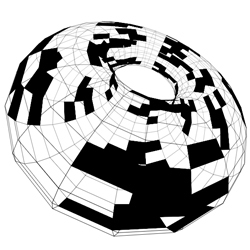
\includegraphics[scale=0.9]{./images/torus-2}
\caption{3D cellular automata with toroidal cellular space.}\label{torus}
\end{wrapfigure}
candidate class of such systems and are well suitable for the modellation and
simulation of a wide class of systems, in particular those ones constructed from
\textbf{many identical} components, each (ideally) simple, but together capable
of complex behaviour\cite{Toffoli1984}\cite{toffoli1987}. In literature there
are lots applications of cellular automata in a wide rage of class problems from
gas\cite{Frisch1986} and fluid turbulence\cite{Succi1991} simulation to
macroscopic phenomena\cite{Gregorio1999} like epidemic
spread\cite{Sirakoulis2000}, snowflakes and lava
flow\cite{Crisci2004}\cite{Spataro2010}.
CA were first investigated by S. Ulam working on growth of crystals using
lattice network and at the same time by Von Neumann in order to study
self-reproduction\cite{Neumann1966}; it was not very popular until the 1970 and
the famous Conway's game of life\cite{Conway1970}, then was widely studied on
the theoretical viewpoint, computational universality were
proved\footnote{CA is capable of simulating a Turing machine, so, in theory is
capable of computing every computable problems(Church-Turing
thesis). Game of life, for example was proved to be capable
of simulating logical gates (with special patterns as
\textit{gliders} and \textit{guns})}\cite{Thatcher1970} and then mainly
utilised, after 1980's, as parallel model due to its intrinsically parallel nature implemented on parallel computers\cite{Margolus1986}.




\section{Informal Definition}

Informally a \emph{cellular automata} (CA) is a mathematical model that
consists of a discrete lattice of sites  and a value, the state, that is
updated in a sequence of discrete timestamps (steps) according to some logical rules that
depend on a neighbor  sites of the cell. Hence CA describe systems whose the
overall behavior and evolution of the system may be exclusively described on the basis of local
interactions\cite{wolfram1984}, property also called centrism.
The most stringent and typical characteristic of the CA-model is the restriction
that the local function does not depend on the time t or the place i: a cellular automaton has homogeneous
space/time behavior. It is for this reason that ca are sometimes referred to as
\textit{shift-dynamical} or \textit{translation invariant} systems. From another
point of view we can say that in each lattice site resides a finite state
automaton\footnote{A simple and well know computational model. It has inputs,
outputs and a finite number of states (hence a finite amount of memory);
An automata changes state at regular time-steps.}  that take as
input only the states of the cells in its neighborhood (see figure \ref{amod3Automata}).

\subsection{Cellular space dimension and geometry}
The cellular space is a \emph{discrete} d-dimensional lattice of sites (see
figure \ref{spazioCellulare}).
For 1-D automaton the only way to discretize the space is in a one-dimensional
grid. For automaton with dimensionality higher than 1 the shape of each cell can
be different than squared. In 2D tessellation for example each cell can be
hexagonal or triangular instead of squared. Each tessellation present advantages
and disadvantages. For instance the squared one does not give any graphical
representation problem\footnote{Each cell could be easily mapped onto a
pixel.}, but present problems of anisotropy for some kind of
simulations\footnote{The HPP model for fluid simulation was highly anisotropyc due to the squared tessellation.}\cite{Frisch1986}.
An Hexagonal tessellation can solve the anisotropy problem\cite{wolfram1986} but
presents obvious graphical issues. Often, to avoid complications
due to a boundary, periodic boundary conditions are used, so that a two-dimensional grid
is the surface of a torus (see picture \ref{torus}).


\subsection{Neighborhood}
\begin{figure}
\centering
\caption{Examples of cellular spaces. (a) 1-D, (b) 2-D squared cells,
(c) 2-D hexagonal cells, (d) 3-D cubic cells.}\label{spazioCellulare}
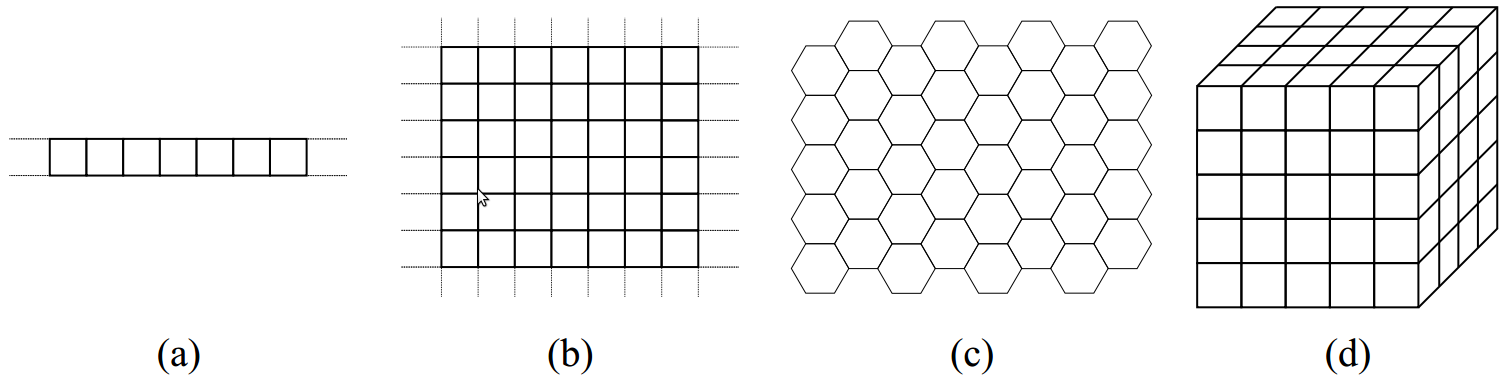
\includegraphics[scale=0.3]{./images/spazioCellulare}
\end{figure}
The evolution of a cell's state is function of the states of the neighborhood's
cells. The geometry and the number of cells that are part of the neighborhood
depends on the tessellation type, but it has to have three fundamental
properties:
\begin{enumerate}
  \item \textbf{Locality}. It should involve only a 'limited' number of cells.
  \item \textbf{Invariance}. It should not be changed during the evolution.
  \item \textbf{Homogeneity}. It has to be the same for each cell of the
  automaton.
\end{enumerate}
Typically neighborhood ``surrounds'' the central cell. For 1-D cellular automata
its borders are identified with a number $r $ called
\textit{radius}\cite{wolfram1983}. A $r=2$ identify
$n=2r+1$ cells in a 1D lattice: the central cell plus the
right and left cells. Typical 2D cellular space neighborhood are the those of
Moore and von Neumann neighborhood. The number of cells in the Moore
neighborhood of range r is the odd squares $(2r+1)^2,$ the
first few of which are 1, 9, 25, 49, 81, and so on as r is increased.
Von Neumann's one consist of the central cell plus the cell at north, south,
east, and west of the central cell itself. Moore's ($r=1$)
one add  the farther cells at north-east, south-east, south-west and north-west
(see figure \ref{mooreNeigh}).



\begin{figure}
\centering
\caption{Examples of different kind of neighborhood with
different radius values.}\label{mooreNeigh}
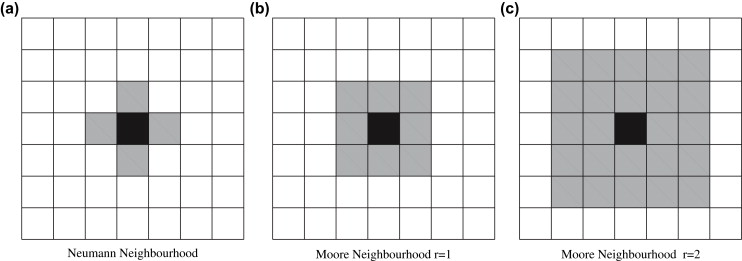
\includegraphics[scale=0.9]{./images/mooreNeigh}
\end{figure}

\subsection{Transition Function}
The evolution of the cell's state is decided by the transition function that
is applied at the same time and on each cell. Usually that transition function
is deterministic and defined by a \textit{look-up} table only when the total
number of state for each cell is small\footnote{Otherwise the dimension of that table would be enormous because the number of entries is exponential in the number of
states.} otherwise is defined by an algorithmic procedure.
It may be probabilistic, in the case of stochastic cellular automata.






\section{Formal Definition}
Cellular automata are dynamic models that are
discrete in time, space and state. A simple cellular
automaton A is defined by a lattice of cells each containing a finite state
automaton so we briefly give its definition.

\subsection{Finite State Automaton}\label{DFA}
Also known as deterministic finite automata (DFAs) or as deterministic finite
state machines, are ones of the most studied and simple computational model
known.
 It is a theoretical model of computation\footnote{Language recognition
problem solvers.} that can be in a finite number of states, only one at a time,
the current state. Its state can change in response of inputs taken by a
transition function that describe the state change given the current state and
\begin{wraptable}{r}{6.0cm}
\scalebox{1.2}{
\begin{tabular}{|c|ccccc|}\hline
\delta & \(a\) & \(b\) & \(c\) & \(d\) & \(e\) \\ \hline
\(q_0\) &\(q_0\) &\(q_0\) &\(q_2\) &\(q_1\) &\(q_1\)\\  
\(q_1\) &\(q_1\) &\(q_3\) &\(q_1\) &\(q_1\) &\(q_1\)\\  
\(q_2\) &\(q_3\) &\(q_2\) &\(q_2\) &\(q_0\) &\(q_1\)\\  
\(q_3\) &\(q_0\) &\(q_1\) &\(q_1\) &\(q_0\) &\(q_1\) \\ \hline 
 \end{tabular}
 }
 \caption{Tabular representation of a DFM's next-state function}
 \label{tab:tabularTransitionFunction}
\end{wraptable} 
the received input of the automata.
Its a much more restrictive in its capabilities than a Turing
machines,\footnote{For example we can show that is not possible for an
automaton to determine whether the input consist of a prime number of symbols.}
but they are still capable to solve simpler problems, and hence to recognize
simpler languages, like well parenthesized string; More in general they are capable
to recognize the so called \emph{Regular languages}\footnote{Languages
defined by regular expressions and generated by regular grammar, Class 3 in
Chomsky classification. We can prove that for each language L accepted by a DFA
exists a grammar $L_G $ s.t. $ L=L_G$},
but they fail for example in parsing \emph{context-free} languages.
More formally a DFA is a 5-tuple:
\[M = <Q,\Sigma,\delta,q_0,F>\] 

\begin{itemize}
  \item \textit{Q} is a finite, nonempty, set of states.
\item $\Sigma$ is the alphabet
\item $ \delta : Q \times \Sigma \longmapsto Q  $ is the
transition function (also called next-state function, may be represented in
tabular form  (see table
\ref{tab:tabularTransitionFunction})
\item $q_0 $ is the initial (or starting) state :
$ q_0 \in  Q $
\item  $F $ is the set, possibly empty, of final states :
$ F \subseteq Q $

\end{itemize}



A run of DFA on a input string $u = a_0,a_1,\ldots,a_n$ is a
sequence of states \\ $ q_0,q_1,\ldots,q_n$ s.t.
$q_i  \overset{a_i}{\longmapsto} q_{i+1} $,
$ 0 \leq i \le n$. It means that for each couple of state
and input the transition function deterministically return the next DFA's
state \\ $q_i=\delta(q_{i-1},a_{i}) $.
For a given word $\textit{w}\in \Sigma^* $ the DFA has a
unique run (it is deterministic), and we say that it \textbf{accepts} w if the
last state $q_n \in F $. A DFA recognizes the
language L(M) consisting of all accepted strings.


Figure \ref{amod3Automata} is an example of DFA\footnote{Graph representation
is the most common way to define and design DFA. Nodes are the states, and
the labelled edges are the possible states transition from a state \textit{u}
to a state \textit{w} given a certain input.
Note that, because the automaton is deterministic is not possible for two
edges to point to two different nodes if same labelled.}.
It accepts the language made up of strings with a number N s.t $N
\;mod\; 3 = 0 $
\begin{itemize}
  \item$ \Sigma = \{a,b\}$
  \item $ Q = \{t_0,t_1,t_2\}$
  \item $ q_0 = t_0$
  \item $ F = \{t_0\} $
\end{itemize}


If we execute the DFA on an input string S=\{aaabba\} we can see that at time
t=0 the DFA is in the initial state $t_0$ and the first
symbol of S is read.
The transition function is applied once per each symbol is S
(i.e. $\left\vert{S}\right\vert$). The only rule that match 
the current state and input is $\delta=(t_0,a)=t_1 $ hence the
new state is $t_1$. The DFA accept the string only if  there
is not any input left and the current state is the final state
$q_f$\footnote{Previously we stated that F was a set but
we can assume that there is only one final state
($\left\vert{F}\right\vert=1$), because it is easy prove
that exist a DFA with only one final state given a generic DFA
($\left\vert{F}\right\vert \geq 1$). We add one more state
$q_f$ and for each final state $q_i \in
F$ we define new rules of the type $\delta(q_i,*)=q_f, * \in I $.}.
S is not accepted by the DFA defined in the example \ref{amod3Automata} because
at the end of the computation the reached state is $t_1$
that is not a final state.
 \[
 t_0\overset{\delta(t_0,a)}
 {\longmapsto}t_{1}\overset{\delta(t_1,a)}
 {\longmapsto}t_{2}\overset{\delta(t_2,a)}
 {\longmapsto} t_{0}\overset{\delta(t_0,b)}
 {\longmapsto}t_{0}\overset{\delta(t_0,b)}
 {\longmapsto}t_{0}\overset{\delta(t_0,a)}
 {\longmapsto} t_{1}
\]
On the input $S^1=\{abababb\}$ the DFA accept:
 \[
 t_0\overset{\delta(t_0,a)}
 {\longmapsto}t_{1}\overset{\delta(t_1,b)}
 {\longmapsto}t_{1}\overset{\delta(t_1,a)}
 {\longmapsto} t_{2}\overset{\delta(t_2,b)}
 {\longmapsto}t_{2}\overset{\delta(t_2,a)}
 {\longmapsto}t_{0}\overset{\delta(t_0,b)}
 {\longmapsto}t_{0}\overset{\delta(t_0,b)}
 {\longmapsto}\mathbf{t_{0}}
\]
\begin{figure}
\begin{center}
  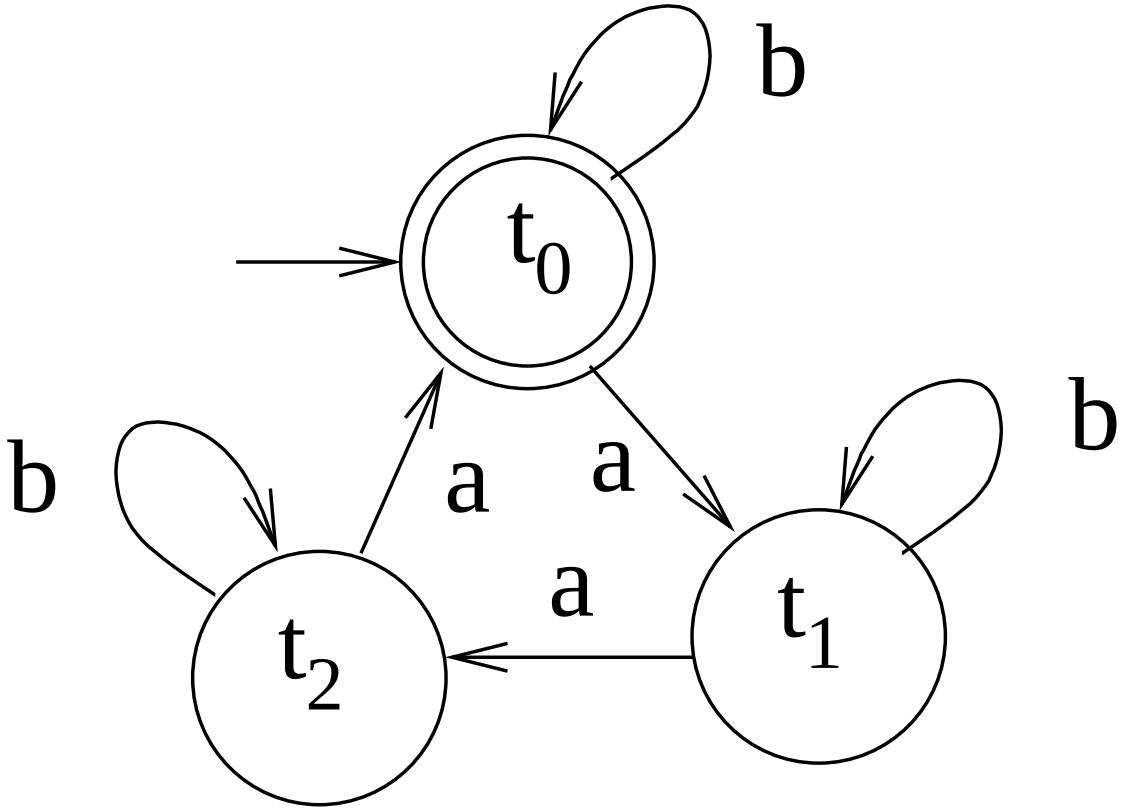
\includegraphics[scale=0.17]{./images/amod3Automata}
  \caption{Graph representation of a DFA}
  \label{amod3Automata}
\end{center}
\end{figure}
\FloatBarrier


\section{Homogeneous Cellular Automata}\label{homogeneousCellularAutomata}
Formally a CA \emph{A} is a quadruple $ A=<Z^d,X,Q,\sigma>$
where:
\begin{itemize}
  \item $\mathbb{Z}^d=\{i=(i_1,i_1,\ldots,i_d)\mid i_k \in
  \mathbb{Z}, \forall k=1,2,\ldots,d \}$ is the set of cells of the d-dimensional
   Euclidean space.
  \item $X$ is the neighborhood, or neighborhood template; a
  set of m d-dimensional vectors (one for each neighbor)
  \[\xi_j=\{\xi_{j1},\xi_{j2},\ldots,\xi_{jd}\} \;,\: 1\leq j \leq m\] that
  defines the set of the neighbors cells of a generic cell
  $i=(i_1,i_1,\ldots,i_d)$
  \[
  N(X,i)=\{i+\xi_0,i+\xi_2,\ldots,i+\xi_d\}
  \] where $\xi_0$ is the null vector. It means that the
  cell $i$ is always in its neighborhood and we refer to it
  cell as \emph{central cell}  (see example below).
\item Q is the finite set of states of the elementary automaton EA.
  
  \item $\sigma=Q^m \rightarrow Q $ is the transition
  function of the EA. $\sigma$ must specify
  $q_k \in Q $ as successor  state of the central cell.
  If there are $m$ cells in the neighborhood of the central
  cell including itself, then there are
  ${\left\vert{Q}\right\vert}^m$ possible neighborhood's
  state configuration. It  means that there are
  ${\left\vert{Q}\right\vert}^{{\left\vert{Q}\right\vert}^m}$
  possible transition functions. Plus we can see that the tabular definition of
  the next-state function is unsuitable for practical purpose. It should have
  $\left\vert{\sigma}\right\vert={\left\vert{Q}\right\vert}^m$
  entries, an exceedingly large number.
  \item $\tau=C \longrightarrow C \longmapsto
  \sigma(c(N(X,i)))$ where $C=\Set*{c}{c \colon Z^d
  \rightarrow Q}$ is called the set of the possible configuration and 
  $
  C(N(X,i)))$ is the set of states of the neighborhood of \textit{i}.
\end{itemize}




For example consider a 2D cellular automata with Moore neighborhood and a
generic cell c=(10,10) and ${\left\vert{Q}\right\vert}=5$
possible state for each cell .
\[X=\{\xi_{0},\xi_{1},\xi_{2},\xi_{3},\xi_{4},\xi_{5},\xi_{6},\xi_{7},\xi_{8}\}
=\]\[=\{(0,0),(-1,0),(0,-1),(1,0),(0,1),(-1,-1),(1,-1),(1,1),(-1,1)\}
\]
Hence the set of the cells belonging to the neighborhood(defined by X) of
c=(10,10) is:
$V(X,c)=\{(0,0)+c,(-1,0)+c,(0,-1)+c,(1,0)+c,(0,1)+c,(-1,-1)+c,(1,-1)+c,(1,1)+c,(-1,1)+c\}
$ 
\[=\{(10,10),(9,10),(10,9),(11,10),(10,11),(9,9),(11,9),(11,11),(9,11)\}
\]
and the total number of entries for the tabular definition of the
transition-function is  ${\left\vert{Q}\right\vert}^{\left\vert{X}\right\vert}=
5^9=1953125$ and the total number of possible transition functions
is
${\left\vert{Q}\right\vert}^{{\left\vert{Q}\right\vert}^{\left\vert{X}\right\vert}}=
5^{5^9}=5^{1953125}$.



\section{Theories and studies}

\subsection{Elementary cellular automata}
The most simple AC we can imagine are the elementary cellular
automata\cite{wolfram1983}. They are one-dimensional periodic N cells array
$\{C_i \mid 1\leq i \leq N, C_i \in \{0,1\} \}$ each
with 2 possible state (0,1), and rules that depend only on nearest neighbor
value hence a radius r=1 neighborhood with a total number of involved cell
$2r+1=2\times1+1=3$ (central, right and left cells).
Since there are only $2\times2\times2\times=2^{2r+1}=2^3=8$ possible states for
the neighborhood of a given cell there are a total of
$2^{2^3}=2^8=256$ possible elementary automata (each of
which may be identified with a 8-bit binary number\cite{wolfram2002}).

\subsubsection{Wolfram's code}
The transition function  is $F(C_{i-1},C_i,C_{i+1})$ is
defined by a look-up table of the form stated in table
\ref{wolframcodeGeneral}, and an example of an instance of a function is given
(rule 110, an important rule on which \cite{cook2004} proved universal
computational power, as Wolfram had conjectured in 1985, and is arguably the
simplest Turing complete system\cite{wolfram2002}) in table
\ref{wolframcodeGeneral}.

\begin{table}
\caption{Encoding of a transition function for a generic elementary CA. On the
right the instance 110.}
\centering
\begin{tabular}{l}
\label{wolframcodeGeneral}

\hfill \\
\hline
  $F(1,1,1)=\{0,1\}$  \\
  $F(1,1,0)=\{0,1\}$  \\
  $F(1,0,1)=\{0,1\}$  \\
  $F(1,0,0)=\{0,1\}$  \\
  $F(0,1,1)=\{0,1\}$  \\
  $F(0,1,0)=\{0,1\}$  \\
  $F(0,0,1)=\{0,1\}$  \\
  $F(0,0,0)=\{0,1\}$  \\
\hline
\end{tabular}
\quad
$\overset{instance}{\longrightarrow}$
\begin{tabular}{l}

\label{wolframcoderule}
\hfill \\
\hline
  $F(1,1,1)=0$  \\
  $F(1,1,0)=1$  \\
  $F(1,0,1)=1$  \\
  $F(1,0,0)=0$  \\
  $F(0,1,1)=1$  \\
  $F(0,1,0)=1$  \\
  $F(0,0,1)=1$  \\
  $F(0,0,0)=0$  \\
\hline
\end{tabular}
\end{table}

More generally Wolfram's code\cite{wolfram1983,wolfram2002} can be calculated 
Conventionally neighborhoods are sorted in non-decreasing order
,(111=7),(110=6),(101=5) etc., and the may be interpreted as a 8-digit number
\[01101110=2^0\times0+2^1\times1+2^2\times1+2^\times1+2^4\times0+2^5\times1+2^6\times1+2^7\times0=110\]


\begin{enumerate}
  \item List and sort in decreasing numerical (if interpreted as number) order
  all the possible configuration of the neighborhood of a given cell.
  \item For each configuration, list the state which the given cell will have,
  according to this rule, on the next iteration.
  \item Interprets the resulting list as binary number and convert it to
  decimal. That  is the Wolfram's code.
\end{enumerate}

Note that is not possible to understand from that code which is the size or the
shape of the neighborhood. Is tacit to suppose that those information are
already known.


\subsection{Wolfram's classification}
Mathematical analysis of CA may be not so straightforward despite their simple
definition. A first attempt to classify CA was attempted by
Wolfram\cite{wolfram2002}. He proposed a set of four classes for CA
classification that are the most popular method of CA classification, but they
suffer from a degree of subjectivity. Classification is based only on visual
valuations, that are obviously subjective. A more rigorous definition of these
classes is given in \footnote{They prove that decide the class(from the
wolfram's four one) of membership of a generic CA is an undecidable problem. Is
not possible to design an algorithm that solve this problem.}\cite{culik1998}.
Here the four Wolfram's classes.
\begin{enumerate}
  
  \item these CA have the simplest behavior; almost all initial conditions
  result in the same uniform initial state (homogeneous state).
  \item different initial conditions yield different final patterns, but
  these different patterns consist of an arrangement of a certain set of
  structures, which stays the same forever or repeats itself within a few
  steps(periodic structures).
  \item behavior is more complicated and appears random, but some repeated
  patterns are usually present (often in the form of triangles)(chaotic pattern).
  \item in some respects these are the most complicated class; these behave
  in a manner somewhere in between Class II and III, exhibiting sections
  both of predictable patterns and of randomness in their pattern
  formation(complex structures).
\end{enumerate}
He observed that the behavior of a meaningful class of Cellular Automata
by performing computer simulations of the evolution of the automata starting
from random configurations. Wolfram suggested that the different behavior of
automata in his classes seems to be related to the presence of different types
of attractors.

 
In figures \ref{class12} and \ref{class34} some elementary automata divided
in their classes.\footnote{Images courtesy of
\url{http://plato.stanford.edu/entries/cellular-automata/}}

 \begin{figure}
 \caption{Class 1 (a,b) and 2 (c,d) elementary cellular automata}
 \label{class12}
\centering
        \subfigure[Rule 250]{%
            \label{fig:first}
            \setlength{\fboxrule}{1pt}%
             \fbox{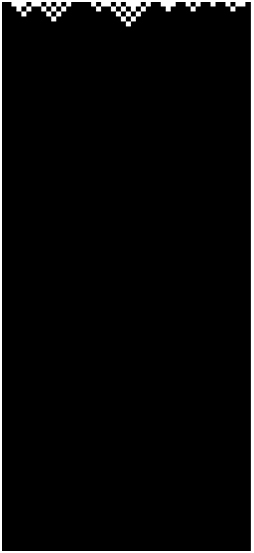
\includegraphics[scale=0.32]{./images/rule250}}
        }%
        \subfigure[Rule 254]{%
           \label{fig:second}
           \setlength{\fboxrule}{1pt}
           \fbox{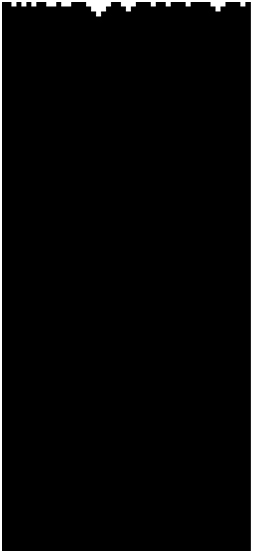
\includegraphics[scale=0.32]{./images/rule254}}
        } %  ------- End of the first row ----------------------%
         \subfigure[Rule 4]{%
            \label{fig:first}
            \setlength{\fboxrule}{1pt}
             \fbox{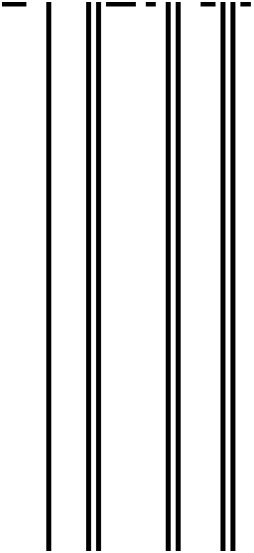
\includegraphics[scale=0.32]{./images/rule4}}
        }%
        \subfigure[Rule 108]{%
           \label{fig:second}
           \setlength{\fboxrule}{1pt}
           \fbox{ 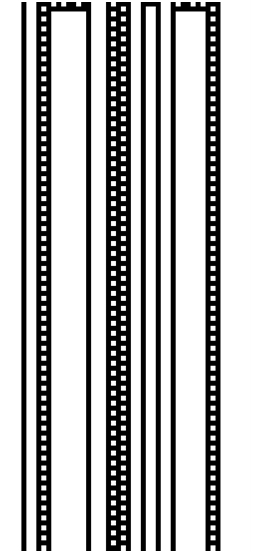
\includegraphics[scale=0.32]{./images/rule108}}
        }\\ %  ------- End of the first row ----------------------%
            
\end{figure}

We can well see from these examples that automata from class 1 have all cells
ending up very quickly with the same value, in a homogeneous state and automata
from class 2 with a simple final periodic patterns.
Class 3 appear to be chaotic and non-periodic and automata from class 4 have
a mixed behaviour, complex-chaotic structures are locally propagated.
\subsection{At the edge of Chaos}
Class 4 automata are at \emph{the edge of chaos} and give a good metaphor for
the idea that the \textit{interesting} complexity (like the one exhibit by
biological entities and their interactions or analogous to the phase transition
between solid and fluid state of the matter, is in equilibrium between
stability and chaos\cite{Langton1990}.

\begin{quotation}
\em Perhaps the most exciting implication (of CA representation of biological
phenomena) is the possibility that life had its origin in the vicinity of a
phase transition and that evolution reflects the process by which life has
gained local control over a successively greater number of environmental
parameters affecting its ability to maintain itself at a critical balance point
between order and chaos.\\
(\textit{\textbf{Chris Langton} - Computation at the edge of chaos.
Phase transition and emergent computation - pag.13}).
\end{quotation}

 \begin{figure}
\centering
 \caption{Class 3 (a,b) and 4 (c,d) elementary cellular automata}
\label{class34}
        \subfigure[Rule 30]{%
            \label{fig:first}
            \setlength{\fboxrule}{1pt}%
             \fbox{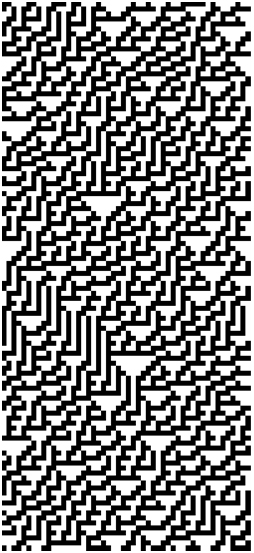
\includegraphics[scale=0.32]{./images/rule30}}
        }%
        \subfigure[Rule 90]{%
           \label{fig:second}
           \setlength{\fboxrule}{1pt}
           \fbox{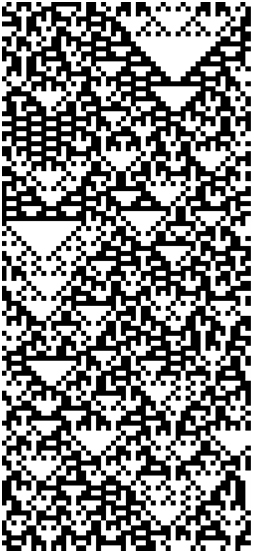
\includegraphics[scale=0.32]{./images/rule90}}
        } %  ------- End of the first row ----------------------%
         \subfigure[Rule 54]{%
            \label{fig:first}
            \setlength{\fboxrule}{1pt}
             \fbox{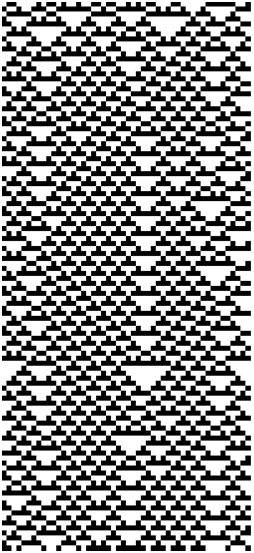
\includegraphics[scale=0.32]{./images/rule54}}
        }%
        \subfigure[Rule 110]{%
           \label{fig:second}
           \setlength{\fboxrule}{1pt}
           \fbox{ 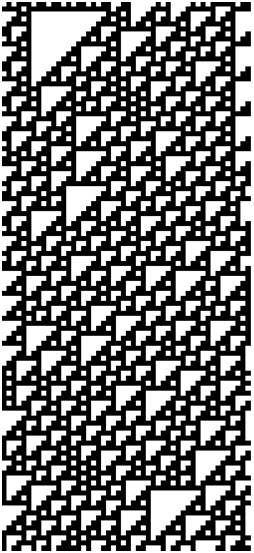
\includegraphics[scale=0.32]{./images/rule110}}
        }\\ %  ------- End of the first row ----------------------%
           
\end{figure}
%%
% -------------- End of figure environment ----------------------%


Langton in his famous paper, \textit{Computation at the edge of chaos: phase
transition and emergent computation}\cite{Langton1990},was able to
identify, simply parametrizing the rule space, the various AC classes, the
relation between them and to ``couple'' them with the classical complexity classes.
He introduced the parameter $\lambda$\cite{LangtonThesis1990}that, informally, is simply
the fraction of the entries in the transition rule table that are mapped  the
not-quiescent state.
\[\lambda=\frac{K^N-n_q}{K^N}\]
where:
\begin{itemize}
  \item K is the number of the cell states
  \item N the arity of the neighborhood
  \item $n_q$ the number of rules mapped to the quiescent
  state $q_q$
\end{itemize}

\begin{figure}
\centering
\caption{Relation between lambda parameter and the CA
behaviors-Wolfram's classes.}\label{lambdaWolframClass}
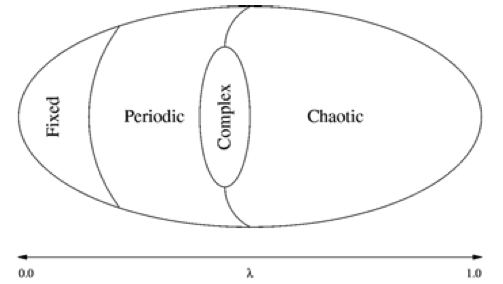
\includegraphics[scale=0.4]{./images/edgeofchaos}
\end{figure}
Langton's major finding was that a simple measure such as it correlates with the
system behavior: as it goes from 0 to $ 1-\frac{1}{K}$(respectively the most
homogeneous and the most heterogeneous rules table scenario), the average
behavior of the system goes from freezing to periodic patterns to chaos and functions with an average 
value of $\lambda$ (see \cite{Langton1990} for a
more general discussion) are being on \emph{on the edge}(see figure \ref{lambdaWolframClass}).

He studied a entire family of totalistic CA with $k=4
$ and $N=5$ with $\lambda$
varying in $[0,0.75]$. He was able to determine that values
of $\lambda\approx0.45$ raise up to class 4 cellular
automata.
Computational system must to provide fundamental properties if it is
to support computation. Only CA  \emph{on the edge} show these properties on
manipulating and store information data.
Here the properties that a computational system as to provide:
\begin{description}
  \item[Storage] \hfill \\
  Storage is the ability of the system of preserving information for
arbitrarily long times
  \item[Transmission] \hfill \\
  Transmission is the propagation of the information in the
form of signals over arbitrarily long distance
  \item[Modification] \hfill \\
Stored and transmitted
information is the mutual possible modification of two signals.

\end{description}

Storage is coupled with less entropy of the system, but transmission and
modification are not. Few entropy is associated with CA of Class 1 and 2 and
high entropy with class 3. Class 4 is something in between, the cells cooperate
and are correlate each other, but not too much otherwise they would be overly
dependent with one mimicking the other supporting computation in all its aspects
and requirements. Moreover class 4 CA are very dependent from the initial
configuration opening to the possibility to encode programs in it.

\subsection{Game of life}\label{sect:GOL}
CA are suitable for representing many physical, biological, social and other
human phenomena. But they are a good tool to study under which condition a
physical system supports the basic operation constituting the capacity to
support computation. Game of life is a famous 2D
cellular automaton of '70s early studied (and perhaps proved) for its universal
computation capacity.



\subsubsection{Game of life - brief definition} 
Game of Life (see figure \ref{gameoflife}) (GOL)\cite{Conway1970} is a
totalistic CA\footnote{A totalistic cellular automaton is a cellular automata in which the rules depend only on the
total (or equivalently, the average) of the values of the cells in a neighborhood.} defined by :
\begin{itemize}
  \item a 2-D lattice of square cells in an orthogonal grid, ideally infinite
  \item $Q=\{0,1\} $ 2 states, and we can picture 1 as
  meaning alive and 0 dead (those interpretation come from the 	
behaviour of the next-state function).
\item $X$ is the Moore neighborhood template.
\item $\sigma$ is the transition function and can be
summarized :
	\begin{itemize}
	  \item \emph{Birth}: If the cell is in the state \textbf{\textit{dead}} and
	  the number of alive neighbors is \textbf{\textit{3}}, then the cell state
	  becomes alive (1).
	  \item \emph{Survival}: If the cell is in the state \textbf{\textit{alive}}
	  and the number of alive neighbors is \textbf{\textit{2 or 3}}, then the cell
	  state is still alive (1).
	  \item \emph{Dead}: If the cell is in the state \textbf{\textit{alive}} and
	  the number of alive neighbors is \textbf{\textit{less than 2 or higher
	  than 3}}, then the cell state becomes dead (0).
	  \end{itemize}
\end{itemize}

GOL is a class 4 Wolfram's taxonomy, rich complex structures, stable blocks and
moving patterns come into existence even starting from a completely random
configuration. 
\begin{figure}
\centering
\caption{GOL execution example.}
\label{gameoflife}
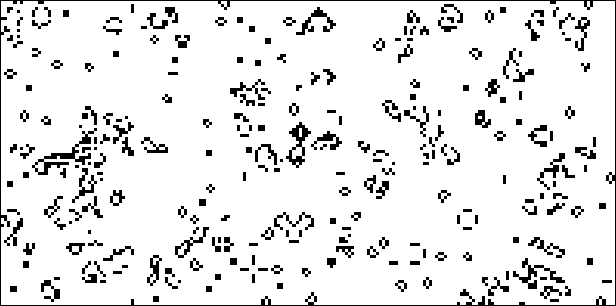
\includegraphics[scale=0.9]{./images/game-of-life}
\end{figure}
\FloatBarrier


A famous block for example is the \emph{glider} ( see picture \ref{fig:glider}) that
is a 5-step-period pattern that is capable of moving into the cellular space.

\subsubsection{Game of life as Turing machine}
Every CA con be considered a device capable of supporting computation and the
initial configuration can encode an input string (a program for example). At
some point the current configuration can be interpreted as the result of the
computation and decoded in a output string. But as we stated before in section
\ref{DFA} not all the computational device have the same computational power. So
which is the one of the game of life? Life was proved can compute everything a
universal Turing machine can, and under Turing-Church's thesis, everything can
be computed by a computer\cite{berlekamp1982}.
\begin{figure}
\centering
\caption{Glider in Conway's game of life.}
\label{fig:glider}
\setlength{\fboxrule}{1pt}%
\fbox{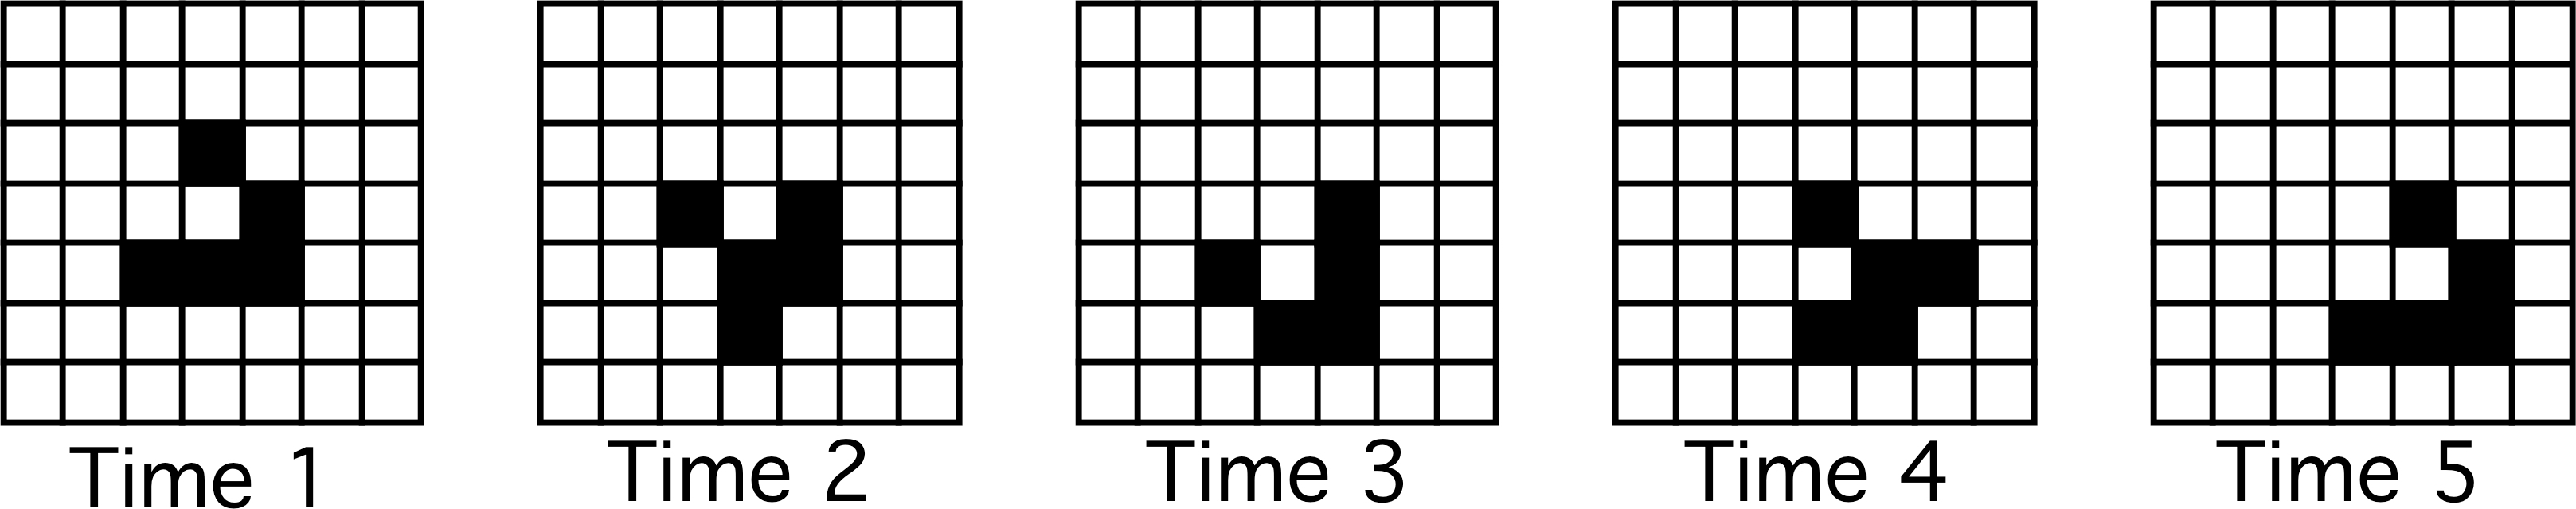
\includegraphics[scale=0.9]{./images/glider}}
\end{figure}



This raises a computational issue; given the \emph{Halting
Theorem}\footnote{There can not be any algorithm to decide whether, given an
input, a Turing machine will accept or not.} the evolution of \emph{Life} is
unpredictable (as all the universal computational systems) so it means that is
not possible to use any algorithmically shortcuts to anticipate the resulting
configuration given an initial input. The most efficient way is to let the
system run.

\begin{quotation}
\em Life, like all computationally universal systems, defines the most efficient
simulation of its own behavior\cite{Ilachinski2001}
\end{quotation}





\section{Extension of the Cellular automata model}
It is possible to relax some of the assumptions in the general characterization
of CA provided in the ordinary CA definitions and get interesting results.
Asynchronous updating of the cell, non homogenous lattice with different
neighborhood or transition functions.

\subsection{Probabilistic CA}
Probabilist CA is are an extension of the common CA paradigm. They share all
the basic concept of an ordinary homogeneous
CA with an important difference in the transition function.
$\sigma$ is a stochastic-function that choose the next-state
according to some probability distributions. They are used in a wide class of
problems like in modelling ferromagnetism, statistical mechanics
\cite{Vichniac1984} or the cellular Potts model\footnote{Is a computational
lattice-based model to simulate the collective behavior of cellular structures.}


\subsubsection{Cellular automata as Markov process}
Another approach in studying CA, even if it is probably not a practical
way to study the CA is to see CA as a Markov process\footnote{Name for the
Russian mathematician Andrey Markov best known for his work on stochastic
processes.}. A Markov process, is a stochastic process that exhibits
memorylessness \footnote{Also called Markov property.} and it means that the
future state is conditionally independent\footnote{Two event
$A$ and $B$ are independent if
$P(A B)=P(A)P(B)$ or in other words that the conditional
probability $P(A|B)=P(A)$.} of the past.
This property of the process means that future probabilities of an event may be
determined from the probabilities of events at the current time.
More formally if a process has this property following  equation holds:
\begin{align*}
P(X(t_n)&= x \,| X\,(t_1) = x_1,X(t_2) = x_2, \ldots,X(t_{n-1})=x_{n-1}) \\
&= P(X(t_n)=x | X(t_{n-1}=x_{n-1})
\end{align*}

In PCA analysis we are more interested in Markov chain because each cell has a
discrete set of possible value for the status variable.
In terms of chain a CA is a process that starts in one of these states and moves
successively from one state to another. If the chain is currently in state
$s_i$, than it evolve to state $s_j$ at
the next step with probability $p_{ij}$.The changes of state
of the system are called transitions, and the probabilities associated with
various state changes are called transition probabilities usually represented
in the Markov chain transition matrix :
\[
M =
\left( {\begin{array}{cccc}
p_{11} & p_{12} & p_{13} &\cdots \\
p_{21} & p_{12} & p_{23} &\cdots \\
p_{31} & p_{32} & p_{33} &\cdots \\
\vdots & \vdots  &\vdots& \ddots\\
\end{array} } \right)
\]

This could seems to be a good way to analyze the probabilistic CA but, a
small grid  $10\times10$ (common models model use grid
$100\times100$ or larger) identify
$2^{10\times10}$possible states and the resulting matrix
dimension of $2^{10\times10}\times2^{10\times10}$ that is a
very large number!

\chapter{Complex cellular automata}

\section{Introduction}
As stated in the section \ref{cellularAutomataIntroduction} cellular automata
are a very powerful tool for modelling complex-systems and they were adopted as
modelling and simulation paradigm in a wide range of applications like
fluid-dynamical phenomena, gas models \cite{Frisch1986}, or lattice Boltzmann
model \cite{Chopard1999}.
The behavior of those physical systems is well described  by the basic laws
of continuum mechanics (Navier-Stokes for example for fluid-dynamics),
but in some cases, when  they cannot be applied directly without adding
phenomenological assumptions or when the set of differential equation
describing the problem is not amenable to any analytical solution (except for
relaxed or particular instances) numerical solution are required.

Hence, general cases require approximated numerical methods commonly based on
space-time discretization and permitted to enlarge the set of cases which can be
carefully simulated.
But many others problems are still intractable and for those problems is
necessary to adopt new solutions. Numerical methods have became more
popular, as computational power raised up in years, and approaches in order to
overcome the problems regarding differential equations\cite{Toffoli1984} were
studied, but at the same time new methods that exploited principles of parallel
computing were adopted either for reasons of absolute performance or reasons of
cost/performance.

\section{Complex phenomena modellation with cellular automata}
Complex phenomena are different from models like Boltzmann lattice model
because of the lager scale of the space that they take into account, like lava
flow simulation models that evolve on a topographical mountain
region map\footnote{Topographical maps are usually discrete altitude value grid
of square cell not less distant than one or two meters from each other. They are
also called DEM, acronym for Digital Elevation Model}.
CA, as defined in the previous chapter are already suitable for this kind of modeling
but, an extension  was introduced by \cite{Gregorio1999} to better fit the
problem of complex phenomena modellation.


\section{Complex Cellular automata (CCA)}
While classical CA are based upon elementary automata, with few states and a
simple transition function, in order to deal with Complex phenomena it is
often necessary to allow a large number of different states a more complicated
transition. The notion of substate is introduced in the Complex case for
decomposing the state of the cell. The values associated to substates can change
in time either due to interactions among substates inside the cell (internal
transformations) or to local interactions among neighbouring cells.
When considering Complex phenomena, each cell usually maps and correspond to
a portion of space and hence a parameter that define the \emph{size }of the
space that each cell represent is needed and it's natural assume that
the cellular space is never higher than 3 ($d \leq 3$).

\subsection{Parameters}
As said before a spatial mapping between cell size\footnote{In terms of cell
side or apothem in case respectively of square or hexagonal cell grid.} and
portion of space in which the automaton evolves is needed and it is also
reasonable to define a \emph{clock} parameter in order to map each CA step to an
effective amount of time. The choice of \emph{cell size} and \emph{clock} are
related to a particular space-time scale in which the CA model simulate the
phenomena and for this reason it has deeply consequence on the form of the model.
They are called parameters because they are predetermined and constant during
the evolution even if in some case a precise estimation mat be given only
\textit{a posteriori}. Moreover the ``best'' value for a parameter can depends 
on the value of the other parameters and modification in one of them  can have
deep consequences on the behavior of the entire model and may require the
repetition of a parameters set rearranging and recalibration phase.


\subsection{Substates}
The state of the cell has in some ways to reflect all the characteristics that
are relevant for the system's evolution. Each characteristic is mapped
to a substate which admitted values are a finite set\footnote{Continuous
quantities might be approximated by discretizing them. Note that on a computer
that is not a problem because floating point computer representations are
already discretized}.
The set of possible state of the cell is given by the cartesian product of  the
sets of substates, so, 
\[
Q = Q_1 \times Q_2 \times Q_3 \times \ldots \times Q_n
\]
When attempting in modelling complex phenomena with many relevant character-
ics could useful to create an higher hierarchy of substates and so further dividing
substates in sub-substates and taking in mind that the values of the substates are
constants within the space occupied by a cell.

\subsection{Elementary processes}\label{elementaryProcesses}
The transition function has to take into account all the possible processes that
can happen in  Complex phenomena, as physics, chemical etc. So as the state
set was decomposed in substates also the transition function is divided in so
called elementary processes that when applied in concert make up 
transition function that describe the entire process.
Moreover the elementary processes can be divided in :
\begin{description}
  \item[Internal transformations] \hfill \\
  Internal transformation \(T_1,T_2,\ldots,T_l\) define the changes in the
  values of the substates only due to interactions among them (e.g., temperature
  drop in SCIARA-fv3, see section \ref{sect:temperatureDrop}, is function of
  the substate lava thickness) inside the cell or due simply to the elapsing of
  the time (e.g., water loss by evaporation). All cell processes evolution that
  are not due to interaction with other cells can be ``labeled'' as
  \emph{internal transformation}. That is, internal transformation are those
  which would take place if all the cells were independent of each other.

For each internal transformation :
\[ 
  T_i \equiv \sigma_{t_i} \colon  S_{T_{i1}}\rightarrow S_{T_{i2}} \:,\: 1 \leq
  i \leq l
\] 
  where $S_{T_{i1}},S_{T_{i2}} \in \mathcal{P}(Q) $(power
  set of Q) 
  \item[Local/neighborhood interaction] \hfill \\
  Local interaction \(I_1,I_2,\ldots,I_k\) describe transformation due to local
  interaction with the neighborhood cells and are often described in terms of
  flows of some quantities across them.
\[
  I_j \equiv \sigma_{I_j} \colon  S^m_{I_{j1}} \rightarrow S_{I_{j2}} \:,\:
  1 \leq j \leq k
\] 
  where $S_{I_{j1}},S_{I_{j2}} \in \mathcal{P}(Q) $(power
  set of Q) and \(m\) is the number of the neighborhood cells.
\end{description}

The whole phenomenon can be so described by sequentially calculating internal
and local interaction functions. The execution order may be
particularly  for the model evolution and for the results\cite{Ruxton1996}.

\subsubsection{External influences}
In some scenario could it be necessary to introduce some extern influence
from the ``outside" of the automaton point of view. Those kind of influences
cannot be described in terms of local rules and typically require dedicated
functions or procedures to be defined. An example of these kind of influences
could be the lava emission from a vent of a volcano (see section \ref{mcaFormal}
for a formal definition).

\section{CCA - a formal definition}\label{mcaFormal}
Formally a Complex cellular automata CCA A is :
\[
A=<\mathbb{Z}^d,Q,P,X,\sigma,E,\gamma>
\]
where:
\begin{itemize}
  \item $\mathbb{Z}^d=\{i=(i_1,i_1,\ldots,i_d)\mid i_k \in
  \mathbb{Z}, \forall k=1,2,\ldots,d \}$ is the set of cells of the d-dimensional
   Euclidean space.
   \item \(Q=Q_1 \times Q_2 \times \ldots \times Q_n \) is the finite set of the
   finite state automaton and is the cartesian product of all the substates
   \(Q_1, Q_2, \ldots ,Q_n \).
   \item \( P=p_1, p_2, \ldots ,p_l \) is the finite set of the
   parameters
  
   \item $X$ is the neighborhood, or neighborhood template; a
  set of m \(d\)-dimensional
  \[\xi_j=\{\xi_{j1},\xi_{j2},\ldots,\xi_{jd}\} \;,\: 1\leq j \leq m\] that
  defines the set of the neighbors cells of a generic cell
  $i=(i_1,i_1,\ldots,i_d)$
  \[
  N(X,i)=\{i+\xi_0,i+\xi_2,\ldots,i+\xi_d\}
  \] where $\xi_0$ is the null vector.
  
  \item $\sigma=Q^m \rightarrow Q $ is the transition
  function of the cells's finite state automaton . It is divided as specified
  before (see section \ref{elementaryProcesses}) in internal
  transformation,\(\sigma_{T_{1}},\sigma_{T_{1}},\ldots,\sigma_{T_{p}}\), and
  local interactions, \(\sigma_{I_{1}},\sigma_{I_{1}},\ldots,\sigma_{I_{o}}\).
  For each local interaction is possible to adopt a particular neighborhood
  template \(X_{I_k} \;,\; 1 \leq k \leq o \) and the general neighborhood
  template would be : 
\[
   D=\bigcup_{i=1}^{o}\{X_{I_k}\}
\]

\item \(E=\bigcup_{i=1}^{s}\{E_i\} \) is the set of the cells affected by
external influences.

\item \(\gamma=\{\gamma_1,\gamma_2,\ldots,\gamma_w\}\) is the set of the
functions that define external influences.
\[
\gamma_i= \mathbb{N} \times E_i \times Q \rightarrow Q \;,\; 1 \leq i \leq w
\]
where \(\mathbb{N}\) is the set of natural number, representing the current
step of the CCA.
  
  
\end{itemize}


\chapter{SCIARA-fv3 - Model Formalization}\label{sect:SCIARA_MODEL}

\section{Model Overview}
Sciara-fv3 is the latest release of the Sciara family of
Complex Cellular Automata Models for simulating basaltic
lava flows. As its predecessor, Sciara-fv2, it is
based on a Bingham-like rheology. However, unlike fv2, it explicitly
computes the flow momentum and the time corresponding
to the computational step (CA clock). In formal terms, it is
defined as:
\[
SCIARA-fv3=<R,X,Q,P,\tau,L,\gamma>
\]

where:

\begin{enumerate}
  \item R is the cellular space, the set of square cells that define the
  bi-dimensional finite region where the phenomenon evolves.
  \item X is the pattern of cells belonging to the Moore
neighborhood that influence the cell state change (see fig.
\ref{fig:mooreNeighModel})
  \item \(Q= Q_z \times Q_h  \times Q_T  \times  Q_{\overrightarrow{p}}  \times
  Q_f^9 \times  Q_{\overrightarrow{vf}}^9  \) is the finite set of states,
  considered as Cartesian product of substates. Their meanings are: cell altitude a.s.l.,
cell lava thickness, cell lava temperature, momentum
(both x and y components), lava thickness outflows
(from the central cell toward the adjacent cells) and
flows velocities (both x and y components), respec-
tively;
  \item \(P = w,t_0, P_T,P_d,P_{hc},\delta,\rho,\epsilon,\sigma,c_v\) is the finite set
of parameters (invariant in time and space), whose
meaning is illustrated in Tab. \ref{tab:parameters}; note that \(P_T , P_d\) ,
and \(P_{hc}\) are set of parameters;
\item \(\tau : Q^9 \longmapsto Q\) is the cell deterministic transition
function; it is splitted in \textit{``elementary processes''}  which, are described
in section \ref{sect:ElementaryProcesses};
\item \(L \subseteq R \) specifies the emitted lava thickness from the source
cells (i.e. craters);
\item \(\gamma : Q_h \times \mathbb{N} \longmapsto Q_h\) specifies the emitted
lava thickness from the source cells at each step \(k \in \mathbb{N}\)
  
\end{enumerate}

\begin{figure}
\begin{center}
  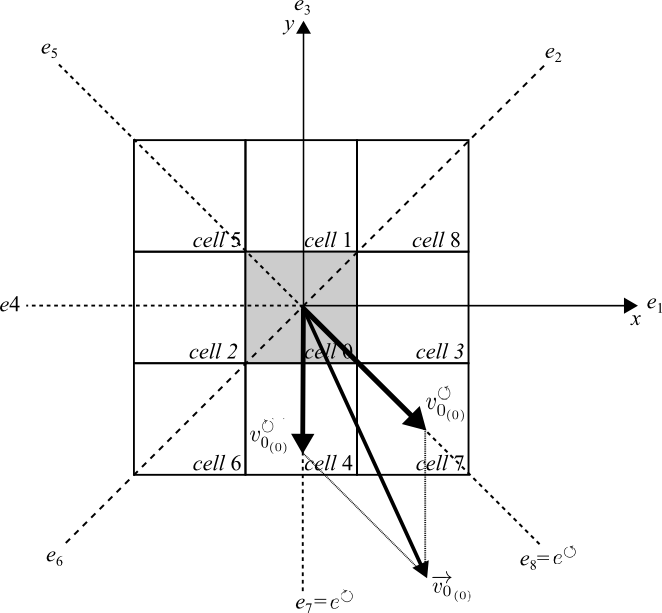
\includegraphics[scale=0.65]{./images/mooreNeighSciaraModel}
  \caption{Example of Moore neighborhood and decomposition of momentum
along the cellular space directions. Cells are indexes from 0 (the central cell,
in grey) to 8. Cells integer coordinates are omitted for a better readability.}
  \label{fig:mooreNeighModel}
\end{center}
\end{figure}


\begin{table}[!t]
% increase table row spacing, adjust to taste
\renewcommand{\arraystretch}{1.3}
% if using array.sty, it might be a good idea to tweak the value of
% \extrarowheight as needed to properly center the text within the cells
\caption{List of parameters of SCIARA-fv3 with values considered for the simulation of the 2006 Etnean lava flow.}
\label{tab:parameters}
\centering
%% Some packages, such as MDW tools, offer better commands for making tables
%% than the plain LaTeX2e tabular which is used here.
\begin{tabular}{l l l l}
\hline
Parameter & Meaning & Unit & Best value\\
\hline
$w$ & Cell side & [m] & 10\\
$t_0$ & Initial CA clock & [s] & 1\\
$t_{\max}$ & Upper value for the CA clock & [s] & 120\\
$P_T$\\
	$\;\;\: T_{sol}$ & Temperature of solidification & [K] & 1143\\
	$\;\;\: T_{vent}$ & Temperature of extrusion & [K] & 1360\\
$P_d$\\
	$\;\;\: dP_{T_{sol}}$ & Dissipation factor at solidification & - & 0.5\\
	$\;\;\: dP_{{T_vent}}$ & Dissipation at extrusion & - & 0.315\\
$P_{hc}$\\
	$\;\;\: hc_{T_{sol}}$ & Critical height at solidification & [m] & 23.066\\
	$\;\;\: hc_{{T_{vent}}}$ & Critical height at extrusion & [m] & 1.014\\
$r$ & Relaxation rate & - & 0.5\\
$\delta$ & Cooling parameter & - & 1.5070\\
$\rho$ & Lava density & [Kg m$^{-3}$] & 2600\\
$\epsilon$ & Lava emissivity & - & 0.9\\
%$\sigma$ & Stephan-Boltzmann constant & [J m$^{-2}$ s$^{-1}$ K$^{-4}$] & $5.68 \cdot 10^{-8}$\\
$c_v$ & Specific heat & [J kg$^{-1}$ K$^{-1}$] & 1150\\
\hline
\end{tabular}
\end{table}

\section{Elementary process}\label{sect:ElementaryProcesses}
\subsection{Elementary process \(\tau_1\): lava flows computation}
The elementary process $\tau_1$ computes lava outflows and their velocities. It is formally defined as:
$$
\tau_1: Q_z^9 \times Q_h^9 \times Q_{\overrightarrow{p}} \to Q_f^9 \times Q_{\overrightarrow{v_f}}^9
$$

Lava flows are computed by a two-step process: the first computes the CA clock,
$t$, i.e. the physical time corresponding to a CA computational step, while the
second the effective lava outflows, $h_{(0,i)}$, their velocities
$v_{f_{(0,i)}}$ and displacements $s_{(0,i)}$ $(i=0,1,...,8)$. The elementary
process $\tau_1$ is thus executed two times, the first one in ``time evaluation
mode'', the second in ``flow computing mode''. Both modes compute the so called
``minimizing outflows'', $\phi_{(0,i)}$, i.e. those which minimize the unbalance
conditions within the neighborhood, besides their final velocities and
displacements. In ``time evaluation mode'', $t$ is preliminary set to a large
value, $t_{\max}$, and the computed displacement, $s_{(0,i)}$, is compared with
the maximum allowed value, $d_{(0,i)}$, which is set to the distance between the
central cell and the neighbor that receives the flow. In case of
over-displacement, the time $t$ must be opportunely reduced in order to avoid
the overflow condition. In case no over-displacement are obtained, $t$ remains
unchanged. Eventually, in ``flow computing mode'', effective lava outflows,
$h_{(0,i)}$, are computed by adopting the CA clock obtained in ``time evaluation
mode'', by guarantying no overflow condition.

\subsubsection{Computation of the minimizing outflows $\phi_{(0,i)}$}\label{sec:min-ouflows}
As in \cite{xxx, xxx}, the initial velocity of the lava inside the cell,
$\overrightarrow{v_{0}}_{_{(0)}}$, is obtained from the momentum components. In
turn, it is decomposed in two components laying over the two directions of the
CA cellular space which are the nearest with respect to
$\overrightarrow{v_{0}}_{_{(0)}}$ itself. These latter directions, which will be
indicated by $e^\circlearrowleft$ and $e^\circlearrowright$, can be found by
moving in counterclockwise and clockwise directions starting from the direction
of $\overrightarrow{v_{0}}_{_{(0)}}$, respectively, as shown in Fig.
\ref{fig:mooreNeighModel}. Thus, if $i$ denotes the $i$-th direction of the cellular
space, $v_{0_{(0)}}^\circlearrowleft$ and $v_{0_{(0)}}^\circlearrowright$ the
modules of the components of $\overrightarrow{v_{0}}_{_{(0)}}$ along the
directions $e^\circlearrowleft$ and $e^\circlearrowright$, respectively, then
the modules of the components of $\overrightarrow{v_{0}}_{_{(0)}}$ along the
directions of the cellular space can be expressed as:
$$ v_{0_{(0,i)}}=
	\begin{cases}
		v_{0_{(0)}}^\circlearrowleft, & \mbox{if }i = e^\circlearrowleft \\
		v_{0_{(0)}}^\circlearrowright, & \mbox{if }i = e	^\circlearrowright \\
		0, & \mbox{otherwise}
	\end{cases}
$$
Moreover, let ${h_k}_{(0,i)} = {v_0}_{(0,i)}^2/2g$ denote the kinetic head associated to the $i$-th component of velocity.

Viscosity effects are modeled in terms of velocity dissipation mechanism, by means of the function $dP$. It depends on temperature and vary according to a power law of the type $\log dP = a+bT$, where $T \in Q_T$ is the lava temperature and $a$ and $b$ are coefficients determined by solving the system (cf. Tab. \ref{tab:parameters}):
$$
\begin{cases}
	\log dP_{T_{sol}} = a+bT_{sol}\\
	\log dP_{T_{vent}} = a+bT_{vent}\\
\end{cases}
$$
Similarly, the relation between critical height and lava temperature can be described by a power law of the kind $\log hc = c+dT$ whose coefficients are obtained by solving the system (cf. Tab. \ref{tab:parameters}):
$$
\begin{cases}
	\log hc_{T_{sol}} = c+dT_{sol}\\
	\log hc_{T_{vent}} = c+dT_{vent}\\
\end{cases}
$$

Before applying the minimization algorithm of the differences for computing the
minimizing outflows, a preliminary control was performed to eliminating cells
that cannot receive lava due to their energy conditions. As in
\cite{Spataro2010}, a topographic correction is considered for flow symmetry
reason. In addition, in Sciara-fv3 the concepts of effective height,
$h_{e_{(0,i)}}$, and apparent height, $h_{a_{(0,i)}}$, was introduced. The first
is the part of $h_{(0)}$ that can really flow out of the cell toward its $i$-th
neighborhood, while the second one is the part which is constrained inside the
cell due to energy conditions. There are three cases (see Fig. \ref{fig:cases}):
\begin{enumerate}
\item if $z_{(0)} + h_{k_{(0,i)}} + h_{(0)} \leq z_{(i)} + h_{(i)}$, then \\
$\begin{cases}
	h_{e_{(0,i)}} = 0\\
	h_{a_{(0,i)}} = h_{(0)}\\
\end{cases}$
\item if $z_{(0)} + h_{k_{(0,i)}} < z_{(i)} + h_{(i)} < z_{(0)} + hk_{(0,i)} + h_{(0)}$, then \\
$\begin{cases}
	h_{e_{(0,i)}} = (z_{(0)} + h_{k_{(0,i)}} + h_{(0)}) - (z_{(i)} + h_{(i)})\\
	h_{a_{(0,i)}} = h_{(0)} - h_{e_{(0,i)}}\\
\end{cases}$
\item if $z_{(i)} + h_{(i)} \leq z_{(0)} + h_{k_{(0,i)}}$, then \\
$\begin{cases}
	h_{e_{(0,i)}} = h_{(0)}\\
	h_{a_{(0,i)}} = 0\\
\end{cases}$
\end{enumerate}
Thus, if denoting with $\theta_{(0,i)} = \arctan ((z_{(0)} + h_{a_{(0,i)}} + h_{e_{(0,i)}}/2) - (z_{(i)} + h_{(i)}))$ the slope angle between the central cell and its $i$-th neighbor (see Fig. \ref{fig:cases}), according to the concept of critical height, the cells for which
$$
h_{e_{(0,i)}} \leq hc \cos \theta_i
$$
are eliminated and cannot receive flow.

The minimization algorithm of the differences is therefore applied to the following quantities, in order to compute the minimizing outflows:

\begin{tabular}{l}
$u_{(0)} = z_{(0)}$\\
$m = h_{(0)}$\\
$u_{(i)} = z_{(i)} + h_{(i)}$
\end{tabular}

The application of the algorithm determines the computation of the minimizing flows, $\phi_{(0,i)}$, from the central cell to the $i$-th neighbor, where $\phi_{(0,0)}$ represents the residual flow which does not leave the cell. Eventually, final velocities and displacements are computed. As a first step, final velocities are computed for each outflow $\phi_{(0,i)}$ $(i=1,2, \ldots, 8)$, by taking into account dissipation:
$$
v_{f_{(0,i)}} = (v_{0_{(0,i)}} + a t)(1-dP)
$$
Here, $a = g \sin \theta$ is the acceleration of gravity, and does not take into account dissipation, which is modeled by the function $dP$. Instead, the final velocity of $\phi_{(0,0)}$ is computed as:
$$
v_{f_{(0,0)}} = v_{0_{(0)}}(1-dP)
$$
In order to compute the displacement, a mean acceleration is computed, which also takes into account dissipation effects: $\overline{a} = (v_{f_{(0,i)}} - v_{0_{(0,i)}})/t$. Therefore, the displacements $s_{(0,i)}$ $(i = 1,2, \ldots, 9)$ are computed as:
$$
s_{(0,i)} = v_{0_{(0,i)}} t + \frac{1}{2} \overline{a} t^2
$$
while, a null displacement is assigned to $\phi_{(0,0)}$:
$$
s_{(0,0)} = 0
$$
since, even if in the real case a movement can occur, inside the discrete context of the cellular space, it is always located at the center of the cell. This is a model simplification which is much more correct as the smaller the size of the cell is.

\begin{figure}[!t]
\centering
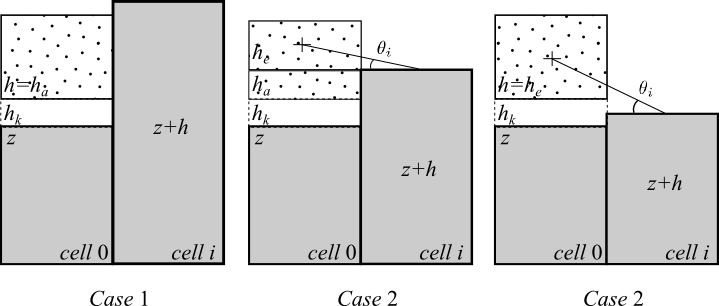
\includegraphics[scale=0.8]{./images/fig2PDP}
\caption{Cases in which the generic neighbor (\textit{cell} $i$) is
eliminated or not eliminated by the minimization algorithm of the difference. If the neighbor is eliminated (\textit{Case} 1), the overall amount of debris inside the central cell is considered as apparent ($h=h_a$), and can not generate an outflow. If the neighbor is not eliminated (\textit{Case} 2 and 3), a part (\textit{Case} 2) or the entire amount of debris (\textit{Case} 3) on the central cell is considered effective ($h \geq h_e$) and can generate outflows. Note that the slope angle $\theta$, considered in the critical height computation, is also shown.}
\label{fig:cases}
\end{figure}

\subsubsection{Time evaluation}\label{sect:modeltimeEvaluation}
Once the minimizing outflows are computed, the CA clock can be determined. As stated above, when $\tau_1$ is executed in ``time evaluation mode'', $t$ is preliminary set to a large value, $t_{\max}$. As a consequence, the computed displacements, $s_{(0,i)}$, can overcome the maximum allowed distance, $w$, i.e. the distance between the central cell and the neighbor that receive the flow. In case of over-displacement, i.e. $s_{(0,i)} > w$, the time $t$ must be opportunely reduced in order to avoid the overflow. The new value of $t$ is determined as follows:

%As a consequence, the computed displacements, $s_{(0,i)}$, can overcome the maximum allowed distance, $d_{(0,i)}$, which is set equal to the distance between the central cell and the neighbor that receive the flow:
%$$
%d_{(0,i)}=
%	\begin{cases}
%		w, & \mbox{if }i \in \{1,2,3,4\} \\
%		w \sqrt{2}, & \mbox{otherwise }\\
%	\end{cases}
%$$
%In case of over-displacement, i.e. $s_{(0,i)} > d_{(0,i)}$, the time $t$ must be opportunely reduced in order to avoid the overflow. The new value of $t$ is determined as follows:

\begin{itemize}
%\item for each minimizing flow, $\phi_{(0,i)}$, a new time, $t_{(0,i)}$, is computed by imposing $s_{(0,i)} = d_{(0,i)}$ and by solving the equation with respect to $t$:
%$$
%t_{(0,i)} = t = \frac{ - v_{0_{(0,i)}} + \sqrt{v_{0_{(0,i)}}^2 + 2 \overline{a} d_{(0,i)}} }{\overline{a}}
%$$
%so that overflow is avoided between the central cell and its $i$-th neighbor;

\item for each minimizing flow, $\phi_{(0,i)}$, a new time, $t_{(0,i)}$, is computed by imposing $s_{(0,i)} = w$ and by solving the equation with respect to $t$:
$$
t_{(0,i)} = t = \frac{ - v_{0_{(0,i)}} + \sqrt{v_{0_{(0,i)}}^2 + 2 \overline{a} w} }{\overline{a}}
$$
so that overflow is avoided between the central cell and its $i$-th neighbor;


\item a new time, $t_j$, is computed in order to avoid overflow conditions along all the neighborhood as:
$$
t_c = \min_{i=1,2, \ldots ,8} t_{(0,i)}
$$
so that overflow is avoided in all the neighborhood;

\item a new minimal time, $t_{opt}$, is computed as:
$$
t_{opt} = \min_{c \in R} t_{c}
$$
in order to avoid overflow conditions over all the cellular space $R$;

\item $t_{opt}$ is multiplied by a relaxation rate factor, $0 < r \leq 1$, for smoothing the phenomenon, and the new CA clock, $\overline{t}$, is obtained:
$$
\overline{t} = t_{opt} r
$$
\end{itemize}

\subsubsection{Outflows computation}
In ``flow computing mode'', minimizing outflows, $\phi_{(0,i)}$, are re-computed by considering the new CA clock $\overline{t}$. Subsequently, lava outflows, $h_{(0,i)}$, are computed proportionally to the displacement, by simply multiplying the minimizing outflow by the ratio between the actual displacement and the maximum allowed:
$$
%h_{(0,i)} = \phi_{(0,i)} \frac{ s_{(0,i)} }{ d_{(0,i)} }
h_{(0,i)} = \phi_{(0,i)} \frac{ s_{(0,i)} }{ w }
$$
Final velocity and displacement are computed as in Section \ref{sec:min-ouflows}.



\subsection{Elementary process $\tau_2$: updating of mass and
momentum}\label{sect:sciaraModelTau2} The elementary process updates lava
thickness and momentum.
It is formally defined as:
$$
\tau_2: Q_f^9 \times Q_{\overrightarrow{v_f}}^9 \to Q_h \times Q_{\overrightarrow{p}}
$$
Once the outflows $h_{(0,i)}$ are known for each cell $c \in R$, the new lava thickness inside the cell can be obtained by considering the mass balance between inflows and outflows:
$$
h_{(0)} = \sum_{i=0}^9 (h_{(i,0)} - h_{(0,i)})
$$

Moreover, also the new value for the momentum can be updated by accumulating the contributions given by the inflows:
$$
\overrightarrow{p}_{(0)} = \sum_{i=0}^9 h_{(i,0)} \overrightarrow{v_f}_{_{(i,0)}}
$$
%while its components along the $x$ and $y$ directions can be simply obtained as:
%$$
%p_{x_{(0)}} = \sum_{i=0}^9 h_{(i,0)} v_{(i,0)} \cos \alpha_{(i,0)}
%$$
%$$
%p_{y_{(0)}} = \sum_{i=0}^9 h_{(i,0)} v_{(i,0)} \sin \alpha_{(i,0)}
%$$	
%being $\alpha_{(i,0)}$ the angle which defines the direction of the velocity of the $i$-th inflow, $h_{(i,0)}$.

\subsection{Elementary process $\tau_3$: temperature variation and lava
solidification}\label{sect:temperatureDrop}

$$
\tau_3: Q_f^9 \times Q_T^9 \to Q_T \times Q_h
$$

As in the elementary process $\tau_1$, a two step process determines the new
cell lava temperature. In the first one, the temperature is obtained as weighted
average of residual lava inside the cell and lava inflows from neighboring ones:
$$
\overline{T} = \frac{ \sum_{i=0}^8 h_{(i,0)} T_i } { \sum_{i=0}^8 h_{(i,0)} }
$$ A further step updates the calculated temperature by considering thermal
energy loss due to lava surface radiation \cite{Park1984}:
$$ T = \frac{\overline{T}}  { \sqrt[3]{1 + \frac{3\overline{T}^3 \epsilon \sigma
\overline{t} \delta}{\rho c_v w^2 h}} } $$ where $\epsilon$, $\sigma$,
$\overline{t}$, $\delta$, $\rho$, $c_v$, $w$ and $h$ are the lava emissivity,
the Stephan-Boltzmann constant, the CA clock, the cooling parameter, the lava
density, the specific heat, the cell side and the debris thickness, respectively
(see Tab. \ref{tab:parameters}). When the lava temperature drops below the
threshold $T_{sol}$, lava solidifies. Consequently, the cell altitude increases
by an amount equal to lava thickness and new lava thickness is set to zero.

Lava flows are computed by a two-step process: the first computes the CA clock, $t$, i.e. the physical time corresponding to a CA computational step, while the second the effective lava outflows, $h_{(0,i)}$, their velocities $v_{f_{(0,i)}}$ and displacements $s_{(0,i)}$ $(i=0,1,...,8)$. The elementary process $\tau_1$ is thus executed two times, the first one in ``time evaluation mode'', the second in ``flow computing mode''. Both modes compute the so called ``minimizing outflows'', $\phi_{(0,i)}$, i.e. those which minimize the unbalance conditions within the neighborhood, besides their final velocities and displacements. In ``time evaluation mode'', $t$ is preliminary set to a large value, $t_{\max}$, and the computed displacement, $s_{(0,i)}$, is compared with the maximum allowed value, $d_{(0,i)}$, which is set to the distance between the central cell and the neighbor that receives the flow. In case of over-displacement, the time $t$ must be opportunely reduced in order to avoid the overflow condition. In case no over-displacement are obtained, $t$ remains unchanged. Eventually, in ``flow computing mode'', effective lava outflows, $h_{(0,i)}$, are computed by adopting the CA clock obtained in ``time evaluation mode'', by guarantying no overflow condition.


\newcommand*{\vttfamily}{%
\fontencoding{T1}\fontfamily{lmvtt}\selectfont
}

\newcommand*{\textsmallunderscore}{%
\begingroup
\fontencoding{T1}\fontfamily{lmtt}\selectfont
\textunderscore
\endgroup
}

\lstdefinestyle{codeStyleC}{
language=C++,
basicstyle=\ttfamily\small,
keywordstyle=\color{blue}\ttfamily,
stringstyle=\color{red}\ttfamily,
commentstyle=\color{green}\ttfamily,
breaklines=true,
columns=flexible,
gobble=4,
xleftmargin=\leftmargini,
frame=L,
numbers=left,
numberstyle=\tiny,
belowcaptionskip=0.5em,
belowskip=1em,
}

\definecolor{darkgreen}{rgb}{0,.5,0}
\lstdefinestyle{codeStyleCUDA}{
language=C++,
basicstyle=\ttfamily\small,
keywordstyle=\color{blue}\ttfamily,
keywordstyle=[2]\color{darkgreen},
keywordstyle=[3]\color{red},
stringstyle=\color{red}\ttfamily,
commentstyle=\color{green}\ttfamily,
breaklines=true,
columns=flexible,
gobble=4,
xleftmargin=\leftmargini,
frame=L,
numbers=left,
numberstyle=\tiny,
keywords=[2]{__global__,__host__,__device__,__synchThreads()},
keywords=[3]{atomicAdd},
belowcaptionskip=1em,
belowskip=1em,
}



\lstdefinestyle{codeStyleFORTRAN}{
language=FORTRAN,
basicstyle=\ttfamily\small,
keywordstyle=\color{blue}\ttfamily,
keywordstyle=[2]\color{darkgreen},
stringstyle=\color{red}\ttfamily,
commentstyle=\color{green}\ttfamily,
breaklines=true,
columns=flexible,
gobble=4,
xleftmargin=\leftmargini,
frame=L,
numbers=left,
numberstyle=\tiny,
keywords=[2]{__global__,__host__,__device__,__synchThreads()},
belowcaptionskip=2em,
belowskip=5em,
}





%chapter start here---------------------------





\chapter{Parallel GPU/CUDA Implementation of the lava flow model SCIARA-fv3}

\section{Introduction}
Parallel computing is a cost-effective method for efficient resolution of
problems and was used as tool for modeling real complex phenomena like a lava
flow, or snowflakes. Many techniques were developed in order to exploit the
power of parallelization differing from each other primarily for the underlying
parallel architecture they are designed for (see chapter
\ref{chap:parallelArchitectures}). In this work we adopted GPUs to accelerate
the SCIARA-fv3 lava flow  (see section \ref{sect:SCIARA_MODEL})cellular
automata model\footnote{A computational model proven to be very suitable for GPU
parallelization.} following the APOD parallelizing methodology (see section
\ref{sect:APOD}) and hence, different parallel versions of the model were
produced, incrementally adopting new features and strategies in order to
achieve better performances.

The versions produced have been:
\begin{description}
\item [\textbf{\textit{Na\"{i}ve implementation :}}] \hfill \\ A basic and simple porting
consisting in mapping each cell of the cellular space to a CUDA
thread. Most part of the scaffolding code was produced here because all the
algorithms and data structures, used in the serial code, that have prevented the parallelism
have been identified and handled (see section \ref{sect:topLevelStrategies} and \ref{sect:naiveImplementation}) .

\item [\textbf{\textit{Rectangular Bounding Box - RBB:}}] \hfill \\ A first
important optimization strategy was adopted here in order to mitigate the
problem of IDLE allocated threads (see section
\ref{sect:idleThreadsDevOccupancy}), that limits the occupancy of the device.
The computation is limited only within the boundaries of a rectangle that has
the property of containing all the active cells (see sections
\ref{sect:serialoptimization} and \ref{sect:RBBOptimization} ) \item
[\textbf{\textit{Shared memory utilization:}}] \hfill \\
A deep analysis on memory accesses was performed to select buffers and
variables more often accessed in kernel code in order to take advantage of the
shared memory (see sections \ref{shareMemory} and
\ref{sect:sharedMemoryOptimization}) \item [\textbf{\textit{Atomic function
implementation:}}] \hfill \\
A family of two versions exploiting CUDA \textit{atomic functions} was developed
as solution to the problem of race-conditions while distributing flows among
cells (see algorithm \ref{alg:distribution})
\begin{enumerate}
  \item \textbf{\textit{RBB-atomic}} : A porting of the RBB version
  introduced before without utilizing the flow's substates (see section \ref{sect:raceCondAvoiding}) for lava flow
  distribution.
  \item \textbf{\textit{List active cells and atomic functions}} : IDLE cells
  and related IDLE threads have been found to be the most prominent limiting
  factor in exploiting GPU power. This version implements a mechanism that tries
  to avoid almost completely this issue, showing very good improvements in
  performances (see section \ref{sect:linearCellAtomic}).
\end{enumerate}
\end{description}


%\subsection{Previous works}
%\label{previousWork}




\section{The Assess, Parallelize, Optimize, Deploy (APOD) design
cycle}\label{sect:APOD}
The Assess, Parallelize, Optimize, Deploy (APOD) is a
cyclical process strategy in parallelizing code. It allows initial speedups to be achieved, with
only minimal initial investment of time (is common that a na\"{i}ve porting of the
application appears to be very easy). The application can be tested, and deployed
at which point the cycle can begin again by identifying further optimization
opportunities, seeing additional speedups, and then deploying the even faster
versions of the application(see figure \ref{fig:APOD}).


\begin{figure}
\begin{center}
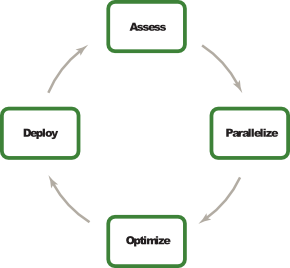
\includegraphics[scale=0.85]{./images/apod-cycle}
\caption[APOD]{APOD design cycle process}
\label{fig:APOD}
\end{center}
\end{figure}

\subsection{Assess}
In this phase, for an existing project the first step is to locate parts of the
code that are responsible for the bulk of execution time, trying to evaluate
bottlenecks and less adapt GPU parallelization parts (see section
\ref{analysysserialCode}).
This way of thinking is a direct consequences of the Amdahl's and Gustafson's
laws (see section \ref{sect:profiling}), and moreover thanks to them the
developer can determine an \textbf{upper bound} of performance improvement from acceleration
of the identified hotspots.

\subsection{Parallelize}
Once hotspots have been identified the developer has to start to parallelize
the code. Depending on the application this goal can be achieved just calling
accelerated libraries (in GPUGPU CUDA environment e.g. cuBLAS or Thrust) or
adding preprocessor directives (e.g. OpenACC or OpenMP). On the other hand,
sometimes in order to fully expose inherent program's parallelism the parallel
porting require some amount of refactoring of the existing serial code.

\subsection{Optimize}
After each round of parallelization the developer can think and move to further
optimize the application. Optimizations can be applied incrementally, and can be
tested in term of speedup achieved and validated.
Optimization can be applied at different level: from the overlapping of memory
transfers with computation to the best block-grid dimensions for a
given kernel in order to augment the occupancy. Profiling and debug tools are
invaluable for this stage of the process as they can suggest the next-best
course of action and provide vital information about the performances.

\subsection{Deploy}
In this phase the developer can compare the outcome with the original
expectations (determined at the \textit{assess} phase). Partial parallelized
program can be carried out for production (this is more important within an
industrial context, because clients can take profit from their investments as
early as possible).

\section{Analysis of the serial code}\label{analysysserialCode}
Undoubtedly, a solid theoretical understanding of the mathematical model and of
the program that actually implements that model (if already exists) are the very
first crucial steps in the process of porting any parallel software.
If the parallelization work starts from an existing code, an analysis phase of
the code itself is fundamental, the reason why this work started from this point.
Cellular automata are well suitable for parallelization, even on GPUs, so the
purpose of this phase is not to determine whether or not the problem is one that
can actually be parallelized but, to identify the program's
\textbf{\textit{hotspots}}, portions of code where most of the work take place
\footnote{Usually scientific and technical programs accomplish most part of the
work, in terms of execution time, is concentrated in few procedures, and
constitute a tiny amount of the whole source code.} and hence concentrates on
parallelizing these hotspots, ``ignoring'' those section of the program that
are not compute intensive in terms of FLOPS. Another important phase is to
identify bottlenecks, areas that could cause parallelizable work to halt or
slowdown (I/O operation are usually something that prevent a full exploiting of
the parallelism, or data dependences), and to possibly restructure those
sections using new approaches, or different algorithms to reduce or eliminate
those bottlenecks.

For example, the problem of calculating the Fibonacci series\footnote{A
particular case of the Fibonacci polynomials F_n(x)=xF_{n-1}(x)+F_{n-2}(x)\)
s.t. \(x=1\) The famous sequence starts with the number 0 and 1 and each
subsequent number is the sum of the previous two. } defined as:
\[ F(n)= F(n-1)+F(n-2), \:\: s.t. \: F(0)=0\;,F(1)=1 \] \[ F(0)\ldots F(17):0,
1, 1, 2, 3, 5, 8, 13, 21, 34, 55, 89, 144, 233, 377, 610, 987, ...
\] is a good example of how an algorithm can deny the parallelization of a
problem. We can see that this approach exposes a too strong data dependence
condition among the values of the series that disallow any possible parallel
implementation because each \(F(n)\) cannot be calculated independently, and
indeed depends of the previous two calculated values.
For example : \hfill \\
\( F(4) = F(4-1)+F(4-2) = (F(4-2)+F(4-3))+(F(4-3)+F(4-4))=
F(4-3)+F(4-4)+F(1)+F(1)+F(0)=F(1)+F(0)+F(1)+F(1)+F(0)=1+0+1+1+0=3 \) to
calculate the \(4\)th element of the series this algorithm needs the 3th and the
2th value. They recurrently need the 2th the 1th, the 0th and so on. It is worth to note that it could be
convenient in this case to change the computation algorithm and using instead of
a recurrent function, a closed formula like the Binet's Fibonacci numbers
formula :
\[ F(n)=\frac{{(1+\sqrt{5})}^n-{(1-\sqrt{5})}^n}{2^n\sqrt{5}} \] or one that use
golden ration \(\phi\) \cite{Wells1986}:
\[ F(n)=
\begin{bmatrix}

\frac{\phi^n}{\sqrt{5}}

\end{bmatrix}
\]
that enables a fully parallelized implementation to take place, enabling two or
more processor to calculate in parallel chunks of the series.

\subsection{Serial code overview}
In this section we'll try to get more into the details of the serial
implementation, in order to better explain the choices taken in parallelizing
the code.


\subsubsection{Memory Organization and data structures}
Working on bi-dimensional cellular automata is not surprising if the
underlying representation of the set \(Q\) of substates is
bi-dimensional as well (see listing \ref{code:memoryPattern2D}) and hence
implemented as:

\lstset{label={code:memoryPattern2D},caption={Substates allocation in serial
code}, style=codeStyleC }
\begin{lstlisting}
	// Substates
	double **Sz;	//Altitude
	double **Sh;	//Lava thickness
	double **nSh;
	double **ST;	//Lava temperature
	double **nST;
	double **SEk;	//Kinetic energy
	double **nSEk;
	\end{lstlisting}
a series of double canonical dynamical C/C++ matrixes for each
substate (we'll see in section \ref{1Dto2Dmemory}
that this memory setting is problematic in CUDA), one for reading cell neighbor
(\textit{updatedCA}) substates and a second for writing the new substate values
(\textit{currentCA}).

Parameters are organized as a series of scalar variables:

\lstset{label={code:memoryPattern2D},caption={}, style=codeStyleC }
\begin{lstlisting}
	double Prho;		//density
	double Pepsilon;	//emissivity
	double Psigma;		//Stephen-Boltzmann constant
	double Pcv;			//Specific heat
\end{lstlisting}

while an abstraction of the vent is given by the class \texttt{TVent} that
encapsulates the class \texttt{TEmissionRate} which store the values, variables
and methods to represent a particular vent emission rate.
The main function of the vent abstraction class is to give back an amount of
produced lava after a certain amount of simulated event's time. The emission of
lava from the vent was discretized into time slot of \(t_e\) and it means that when the simulation time
\(t_s\) is such that \(i t_e \leq t_s < (i+1)  t_e \) the emitted lava thickness
value at the slot number \(i\) is returned.
\lstset{label={code:memoryPattern2D},caption={}, style=codeStyleC }
\begin{lstlisting}
	double thickness(double sim_elapsed_time, double Pt,unsigned int emission_time,
	double Pac) { 
	unsigned int i = (unsigned int)(sim_elapsed_time/emission_time); 
	if (i >= _emission_rate.size())
		return 0;
	else
		return _emission_rate[i]/Pac*Pt;
	}
\end{lstlisting}


\subsubsection{Transition function and elementary processes}
The transition function \(\tau\) and all the elementary processes \(
\tau_1,\tau_2 \ldots \) have  correspondent functions in the code.
\lstset{label={code:memoryPattern2D},caption={}, style=codeStyleC }
\begin{lstlisting}
	void GlobalTransitionFunction();
	void SwitchToHeat();
	void empiricalFlows();
	void getInitialVelocities(const int& x, const int& y, double* v);
	double outflowsProp(int x, int y, double *f, double *v, double *p, bool T_or_F);
\end{lstlisting}

The transition function consist of ordered calls to the \(\tau_1,\tau_2 \ldots
\) procedures. One of them, \texttt{empiricalFlows()}, is more interesting than
the others because it involves the determination of the temporal step, the
calculation of the superficial flow and their distribution among the cells in
the neighborhood of a central cell.
As stated in section \ref{sect:modeltimeEvaluation} the temporal
computational step is the minimum between all the temporary computational time
step calculated by each cell and the distribution is outlined in the algorithm
\ref{alg:distribution} (for the sake of brevity taking in account only one
substate, the lava thickness, but the same strategy is applied also to the
others):

\begin{algorithm}
\begin{algorithmic}

\FORALL {$c \leftarrow cell$}
\FORALL {$n \leftarrow  neighborhood(c)$}

\STATE $nSh(c) \leftarrow nSh(c)-flow(c,n)$
\STATE $nSh(n) \leftarrow nSh(n)+flow(c,n)$

\ENDFOR
\ENDFOR
	\caption{Distribute lava flow among the neighborhood's cells}
	\label{alg:distribution}
\end{algorithmic}
\hfill\\

where \texttt{flow(c,n)} is the computed superficial flow of lava from the cell
$c$ to the cell $n$ and \texttt{nSh(c)} is the update matrix of the substate thickness.
The lava flow from the central cell \(c\)
to a cell $n$ of the neighborhood is subtracted (reason of the minus sign),
and added to cell $n$ itself.
\end{algorithm}
Two important information arise from the analysis of this function:
\begin{itemize}
  \item At each step a minimum value has to be found among all the cell of
  the cellular space; in a parallel context this should be carried out by means
  of some reduction algorithm.
  \item This distribution approach is not suitable for a direct porting due to
  the obvious race condition problems.
\end{itemize}
We will take in account these and other problems in section
\ref{sect:raceCondAvoiding}.

\subsubsection{Serial Optimizations}\label{sect:serialoptimization}
This way of updating the cellular space, although it does not fit perfectly with
the theoretical cellular automata model, may be considered as an optimization
because otherwise a set of nine flow substates should be stored and managed to
keep track of the substates quantities interchanged at each step.
Moreover the transition function is applied only on cells where the thickness
substate value \(sh_{cell} > 0 \). The cellular space could be formed by a very
large number of cells (for example we applied the model to a discretization of a
flank of Mount Etna corresponding to a \(517 \times 378 = 195426\) cells
cellular space), but in the context of ``evolutive'' phenomena such as volcano
eruptions and consequent lava flow modelling, that evolve starting from only a
limited active part of the space and growing as the time passes by, cells that
are far from lava are considered to be \textit{idle} because they cannot be
neither sources nor receivers of any lava quantity, consequently skipping their
computation would not affect the final result. Hence minimizing the number of
times in which transition function is applied on idle cells could be crucial for
performances and in a serial programming context this can be accomplished easily
without any overhead.
The listing \ref{code:skypIdleCell} shows how a serial implementation of the
cellular automata loops over the cellular space and it selectively applies the
transition function whether the \texttt{if} predicate \(sh_{cell} > 0 \) is
true.
The most computationally intesive part of the transition function is so avoided
for such cells.
\lstset{label={code:skypIdleCell},caption={Selective applying of the transition
function on active cells.}, language=C++, basicstyle=\footnotesize\ttfamily,
keywordstyle=\color{blue}\ttfamily, keywordstyle=[2]\color{darkgreen},
stringstyle=\color{red}\ttfamily, commentstyle=\itshape\color{green},
breaklines=true, frame=L, columns=flexible, gobble=4, xleftmargin=\parindent,
belowcaptionskip=1em, belowskip=1em, }
\begin{lstlisting}
	for (int x = 0; x < COLS ; x++)
		for (int y = 0; y < ROWS ; y++)
		if (Sh[x][y] > 0 ) {
			...
			/*HEAVY WORK*/
			...
\end{lstlisting}


Hence from here it's clear that the minimization of the idle cells computation
is an important optimization and we'll see in sections \ref{sect:RBBOptimization} and
\ref{sect:linearCellAtomic} that this idea is still valid in a parallel context.

\subsection{Profiling - Gprof}\label{sect:profiling}
Bottlenecks can be identified by performing the profiling analysis of the code.
Profiling consist of a numbers of metrics that describe the complexity of an
application in term of space and time. Profiling is achieved using tools called
\textit{code profilers}.
The output of a profiler usually consist of a :
\begin{description}
\item[Statistical summary:]\hfill \\
The profiler annotates statistics and metrics against the source
code statements when a certain event occurs (e.g. a method call or an
\texttt{else} part of a \texttt{if} branching). It can record for example the
entire trace of the called methods in a so called \textit{call graph} (see figure \ref{stackCall}). A call
graph is a direct graph describing relations between subroutines. It could be:
\begin{itemize}
  \item \textbf{dynamic}
  Is dynamic when the graph is a record of an execution of the program.
  \item \textbf{static}
  Static call graph are built ``offline'' and it intends to represent
  \textbf{every} possible run of the program. Building an exact static call
  graph is an undecidable problem so usually they are approximations. An
  example of tools that perform static call graph analysis are
  \textit{cflow}\footnote{\url{https://lists.gnu.org/archive/html/info-gnu/2011-10/msg00010.html}}
  and
  \textit{egypt}\footnote{\url{http://www.gson.org/egypt/}}
\end{itemize}
\end{description}

For this work the profiling tool Gprof was used. It is a Unix tool that allows
to compute a large number of statistics and a dynamical call graph. There was no
need for any static graph call analysis because the purpose of using a profiling tool was not to
understand the behavior of the program but to find the possible bottlenecks and
hotspots. It works injecting instrumentation code automatically into the code (
compiling\footnote{Gprof can be used only with compatible compilers like G++}
with the option \textit{-pg}) like for example a call to a monitor function
\textit{mcount}\footnote{This function may not be thread safe in some
implementation, so can produce incorrect results.} before each function call.
At the end of the execution a file with extension \textit{.gmon}
(program\_name.gmmon) is saved.
The information is collected simply sampling the execution of the program
probing the target program's \textit{program counter} at regular intervals using
operating system interrupts (programmed via \texttt{profil()} or
\texttt{setitimer()} syscalls).
The overhead related to the profiling with Gprof can vary from 30\% to 250\%
\cite{Froyd2005}.




\subsection{SCIARA-fv3 profiling}
In figure \ref{stackCall} the call graph\footnote{The stack call image was
obtained using the script GProf2Dot that convert profiling output from Gprof to
a dot graph. \url{https://code.google.com/p/jrfonseca/wiki/Gprof2Dot}} coupled
with other metrics is shown as the number of times that a function is called
and the percentage of the total time that a use (we omitted, without losing any critic
informations, functions which the execution time was too short or not directly
related to the computation, e.g. initialization of threads or setting up of
linked list because of readability).
The figure is related to an execution of \(2000\) computational steps of the
model itself.
We can easily see that the \textbf{97\%} (i.e. it may allow a almost fully
parallel implementation) of the computation takes place into function
\texttt{GlobalTransitionFunction()} that is called in total, not surprisingly
2000 times. The top level hotspot is so identified and we can start making some
prediction about the speedup's upper bound according to the Amdahl's law.
Using \(p=512\) cores of a fermi GTX 580 GPU we can expect that the speedup \[
S(512)=\frac{1}{B+\frac{1}{512}(1-B)}\approx31.35, \quad B=1-0.97; \] where B is
the serial portion of the whole program. We cannot expect speedups better than
\(31\times\) even using 512 cores in parallel and without any additional
overhead (at least on 2000 computational steps).
Obviously as the computational steps increase the percentage of the total time
taken by the hotspots \texttt{GlobalTransitionFunction()} becomes closer and
closer to \(100\%\), giving at limit a theoretical speedup limit \(S(p)=p\).
Hence, all the efforts in parallelizing the application have been spent on the
acceleration of this part. Each called procedure in
\texttt{GlobalTransitionFunction()} procedure corresponds to an elementary
process\footnote{We can easily see from the same figure that the most
computationally expensive, among them, is the calculation of the outflows
called 9 times for each cell and computational step.} of the MCA.
\begin{figure}[p] \vspace*{-2cm}
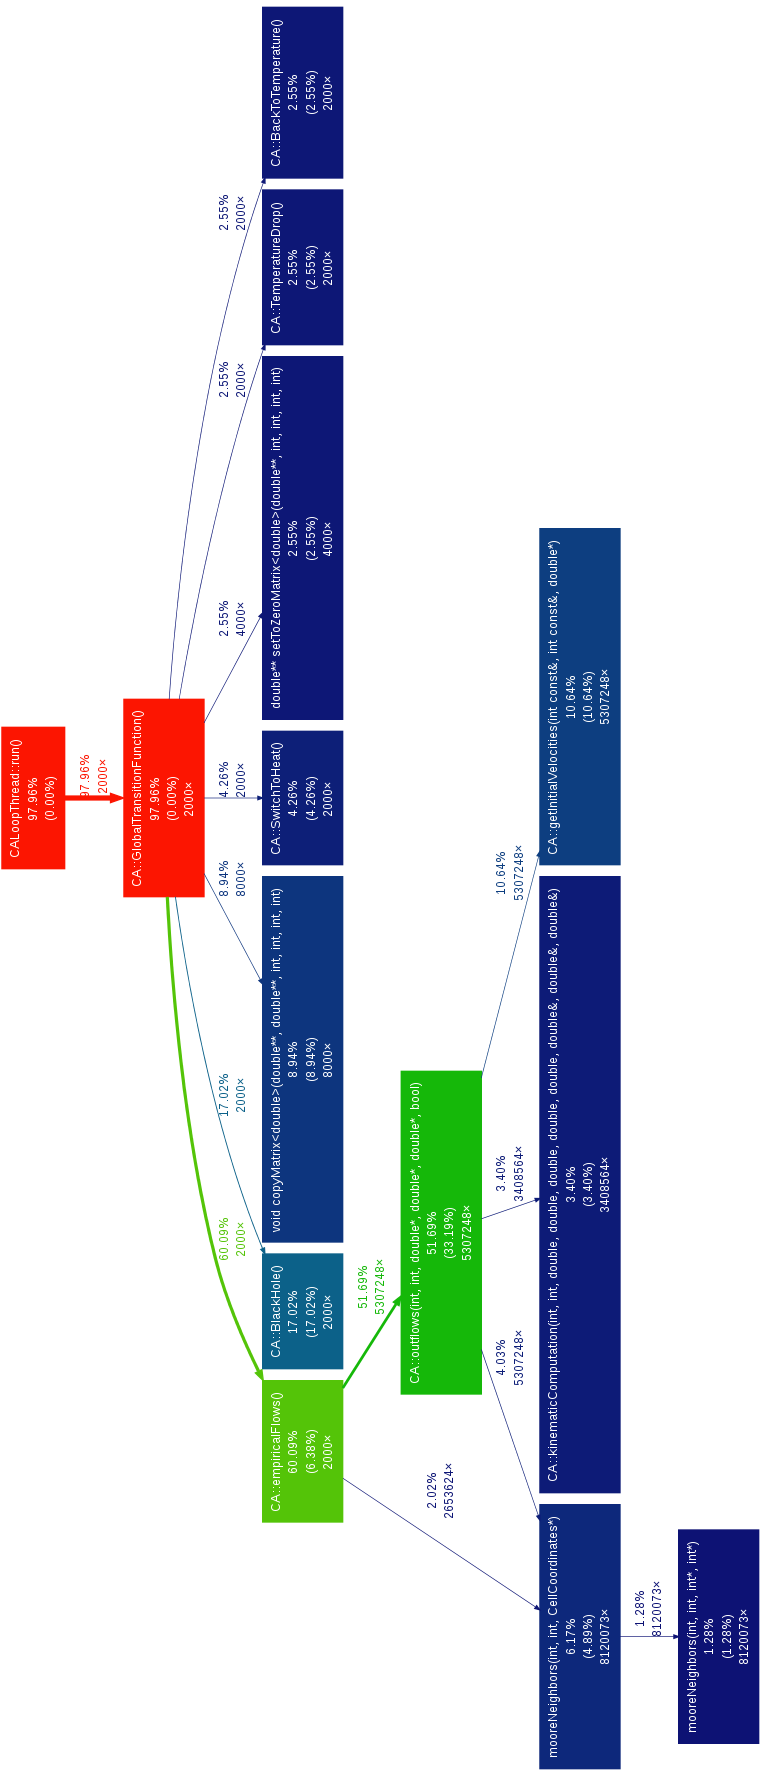
\includegraphics[width=0.67\linewidth]{./images/profiling}
\caption{Call graph for the serial version of the SCIARA-fv3 model}
\label{stackCall}
\end{figure}
Another important information  obtainable from the figure \ref{stackCall} is
that the bulk of computation  is not enclosed in one single very computationally
intensive procedure call (like, for example, could be a single call to a
matrices multiplication, or a differential equation solver procedure), but it
resides in the large number of calls to sub-procedures, (\(\approx5\times10^6\)
calls for the sub-procedures like \texttt{outFlows(\ldots)} in this specific run
of the model).




\section{Top level and strategies overview}

\label{sect:topLevelStrategies}
At high level the workflow of the parallel version consists of (the classic
host-managed accelerated program structure):
\begin{enumerate}
  \item Data structures initialization on CPU (see section \ref{1Dto2Dmemory})
  \item Memory copies \(CPU \rightarrow GPU\)
  \item Global transition function execution on GPU
  \item Results memory copies \(CPU \leftarrow GPU\)
\end{enumerate}

The parallelization strategy design purpose was to avoid as much as possible the
highly undesirable \(CPU \leftrightarrow GPU \) copy operations by means of a
complete execution of all the elementary processes functions on the device and
performing only a \(updatedCA \leftarrow currentCA \) device-to-device copy
operation to re-initialize the \textit{updatedCA} swapping the latter with the
\textit{currentCA} buffers (see section \ref{sect:serialoptimization}).

The elementary processes are the constituent of the global
transition function of the cellular automata and the order in which they are
executed is crucial for the correctness of the final result. They need to be
applied sequentially and hence \(\tau_{i+1}\) can be applied only and only if
\(\tau_{i}\) was already executed. From an implementation point of view this
means that all cells have to first compute the current elementary process before
performing the subsequent one. Hence we decided to map each elementary process
to different CUDA kernels that allow a global synchronization (at grid level),
not interleaving (as soon as they are executed on the same CUDA stream), de
facto, any elementary process function. An example is shown in listings
\ref{code:kernelCalls}.

\lstset{label={code:kernelCalls},caption={Elementary processes kernel
function calls.}, language=C++, basicstyle=\footnotesize\ttfamily,
keywordstyle=\color{blue}\ttfamily,
keywordstyle=[2]\color{darkgreen},
stringstyle=\color{red}\ttfamily,
commentstyle=\itshape\color{green},
breaklines=true,
frame=L,
columns=flexible,
gobble=4,
xleftmargin=\parindent,
belowcaptionskip=1em,
belowskip=1em, }
\begin{lstlisting}
	//crater kernel
	handleVents<<<1,sciaraGPU->params[EN_numVents]>>>(...);
	
	//elementary process #1
	switchToHeat<<<dimGrid,blockSize>>>(...);
	
	//elementary process #2
	empiricalFlow_fill_TIMES<<<dimGrid,blockSize>>>(...);
\end{lstlisting}

In order to exploit the fine-grain parallelism of the CUDA architecture one of
the first issues to decide is the amount of work that a single thread has to be
loaded with, in term of numbers of cells that it has to take into account. For
example one might think to use one thread for a single row or column or in
general for a subset of the cellular space as in a typical data-parallel
application. However while working with CUDA a very high number (thousand or
even millions) of threads should be created in order to exploit the massive
parallel architecture of the GPU\cite{NvidiaprogGuide}. The most common and
widely adopted strategy while working with arrays in CUDA is to map one thread
to one cell and similar approaches are used for example in \cite{dambrosio2012}.
The thread grid and blocks dimension have to be setted to the best value
according to CUDA best practices\cite{CUDACBESTPRACTICE} manual and choosed
utilizing the CUDA provided occupancy calculator spreadsheet (see
\ref{sect:cudaPerfGuideline} at page \pageref{sect:cudaPerfGuideline}). Those
values change from kernel to kernel, and depend on the device actually utilized
and on a number of other factors like the register pressure or the shared memory
utilization. In addition to this analysis, a series of experimentations were
performed in order to find the best set of values to achieve best performances. 
The transition function code may be very thread divergent because of the
complexity of the physical simulation. Another example could be
the if statement, that limits the execution only to the \textit{active} cells,
as talked in section \ref{sect:serialoptimization}.
At step \(t\) the lava is not homogeneously distributed among all the cells, and
it means that it is possible, for two different threads (i.e. cells) in the same
warp, to execute two divergent code paths. In sections
\ref{sect:atomicImplementation}, \ref{sect:RBBOptimization} and
\ref{sect:linearCellAtomic} we discuss some possible solutions in order to
mitigate this issue.
In listing \ref{code:threadDivergentCode} we show an example of a very thread
divergent code within SCIARA-fv3: a multiple \texttt{if-else} inside a loop. Each
thread within a warp can execute a different path at each iteration of the loop at line 1, preventing CUDA to fully
parallelize this section, and executing in serial the thread's subsets of the
warp in which all the threads share the same divergent path. Each subset is then
executed in parallel. In the worst case, when all the threads within a warp
execute a different path, the executions is completely serialized\footnote{CUDA
is SIMT because allow divergent execution path, but, it does not come for free.
A certain amount of serialization is the price to relax the strict SIMD
programming rules, and hence, a good CUDA programmer should avoid as much as
possible those divergent execution paths.}\cite{NvidiaprogGuide}.





\lstset{label={code:threadDivergentCode},caption={Thread divergence code, into
the calculate outflows elementary process function.}, language=C++,
basicstyle=\footnotesize\ttfamily, keywordstyle=\color{blue}\ttfamily, keywordstyle=[2]\color{darkgreen}, stringstyle=\color{red}\ttfamily,
commentstyle=\itshape\color{green},
breaklines=false,
frame=L,
columns=flexible,
gobble=4,
xleftmargin=\parindent,
belowcaptionskip=1em,
keywords=[2]{__constant__,__global__,__host__,__device__,__synchThreads()},
belowskip=1em, }
\begin{lstlisting}
    for (int i = 1; i < MOORE_NEIGHBORS; i++) {
	i < VON_NEUMANN_NEIGHBORS ? zc[i] = z[i] : zc[i] = z[0]-(z[0]-z[i])/rad2;

	// ha and he evaluation
	if (z[0] + hkr + hk[i] + h[0] <= zc[i] + h[i]) {
		he[i] = 0;
		ha[i] = h[0];
	} else if (z[0] + hkr + hk[i] >= zc[i] + h[i]) {
		he[i] = h[0];
		ha[i] = 0;
	} else if (z[0] + hkr + hk[i] + h[0] > zc[i] + h[i]) {
		he[i] = (z[0] + hkr + hk[i] + h[0])-(zc[i] + h[i]);
		ha[i] = h[0] - he[i];
	}
	i == 0 ? w[i] = 0 : w[i] = Pc;
	theta[i] = atan(((zc[0]+ha[i]+he[i] / 2.0) - (zc[i]+h[i])) / w[i]);
	w[i] = w[i] / cos(theta[i]);
	}

\end{lstlisting}

Regarding the mapping between the data structures and the CUDA memories we
followed the CUDA best practice manual\cite{CUDACBESTPRACTICE} advices.
Substates are arrays whose dimensions are only suitable for global memory
memorization whilst for parameters we decided to utilize constant memory (see
section \ref{sect:constantmemory} at page \pageref{sect:constantmemory}) due to
their intrinsically constant nature and their access rate in the code.
Moreover, all the constant variables of the automata have been stored in this
memory like for instance \(x\) and \(y\) dimension's sizes of the cellular space
which, although not strictly parameters, are constant while
the execution of the model, from the beginning to the end of the simulation. In listings
\ref{code:constantDeclaration} the declaration of the array stored in constant
memory is shown.
Note that it is an automatic array, and its dimension has to be known at compile
time and so an analysis phase was needed to select all the candidate variable to
be stored in that buffer.

\lstset{label={code:constantDeclaration},caption={Thread divergence code, into
the calculate outflows elementary process function.}, language=C++,
basicstyle=\footnotesize\ttfamily, keywordstyle=\color{blue}\ttfamily, keywordstyle=[2]\color{darkgreen}, stringstyle=\color{red}\ttfamily,
commentstyle=\itshape\color{green},
breaklines=false,
frame=L,
columns=flexible,
gobble=4,
xleftmargin=\parindent,
belowcaptionskip=1em,
keywords=[2]{__constant__,__global__,__host__,__device__,__synchThreads()},
belowskip=1em, }
\begin{lstlisting}
	#define NUM_PARAMS 21
	enum { EN_Pc1, EN_Pac1, EN_PTsol1, ... ,EN_LX1,EN_LY1};	
	__constant__ float d_params[NUM_PARAMS];

\end{lstlisting}


The main program and all the kernels are organized in C style manner in the
sense that CUDA does not allow C++ features such as classes utilization in its
code.
Thus, two c-99 structs have been created and combined to recreate the serial SCIARA-fv3 object
structure. They store a double copy of all the data, a CPU and GPU
version\footnote{Note that those double copies are different from the pair of
buffers that are needed for updating the next CA configuration at each step.
Here we are referring to a mirror copy of each variable we find in GPU device memory,
because at the beginning, at the end and sometimes in the middle of the
execution we need to perform some buffers copies that require a CPU version of
the buffers.}.
The original data structures are first copied into the new CPU data structures
in order to be copied and mapped into the GPU buffers.

\begin{enumerate}
  \item \texttt{SCIARA\_GPU}  : Main struct of the model, in which all the
  data structures are declared, created and destroyed. It is provided also with
  a method that allows the initialization of all the buffers from the CPU
  version of the model (that actually do the reading of all the initial
  configurations and parameters). It also contains an instance of the structure
  \texttt{SCALAR\_GPU}, that manages all the scalar values.
  \item \texttt{SCALAR\_GPU}: All the scalar values and methods that are related
  to them (like truncation or mathematical operations) are stored in this
  structure.  It is enclosed into the main structure of the program and managed by it.
\end{enumerate}

As stated in section \ref{sect:APOD} the assess phase of the development
consists also in locating possible parts of the code that are not very suitable for a
parallel implementation, either in terms of possible race-conditions or strategy
and algorithms, adopted in the serial version, that could limit the total amount
of parallelism that can be achieved. The most evident parallel implementation
limitation is related to the bi-dimensional data structures used in the serial
version. In the following section \ref{1Dto2Dmemory} we discuss more in detail
this issue and its solutions.

\subsection{Migration from 2D matrices to linear arrays}
\label{1Dto2Dmemory}
The first problem that was faced regarded the data organization in memory.
2D matrices are not allocable in the CUDA framework, which gives only the
possibility to allocate linear arrays within the global memory
\ref{memoryModel}. We first produced a serial version of the model that uses
only 1D arrays using an explicit row-major representation\footnote{Row-major is the internal
memory representation adopted in C/C++ languages to store automatic matrix
that are stored in a linear e continuous space in memory. Dynamic matrices are
usually managed allocating vector of pointers each representing a row. This
approach only store the data within a row in contiguous space, but spread the
rows into the heap space}; it involves the transformation of the cell
coordinate from 2D to a scalar number.
Given a 2D matrix of dimension \(D_y,D_x\) where \(D_y\) is the number of
rows and \(D_x\) is the number of columns and a cell of 2D coordinates
\(C_{2D}=(y,x)\) the scalar 1D coordinate is obtained using \(c_{1D}=yD_x+x\).
Cells are stored in a linear array such that rows are memorized one after the
other.
For example see figure \ref{fig:rowMajor}. 
\begin{figure}
\begin{center}
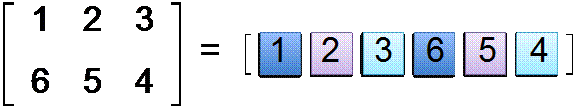
\includegraphics[scale=0.45]{./images/rowmajor}
\caption{Row-major matrix translation}
\label{fig:rowMajor}
\end{center}
\end{figure}
\FloatBarrier
Note that the same concept of ordering cells in 1D buffers is applicable also to
n-dimensional arrays \(n > 2\).
\subsubsection{Row-Major n-dimensional arrays representation}
Generalizing : If \(A=D_1 \times D_2 \times  \ldots \times D_n\) is a
n-dimensional array and given an element of A specified by a n-tuple \(a=(d_1,d_2,\ldots,d_n)\)
of (indexing start from zero) where \(d_k \in [0, D_k-1]\), the
memory offset in a 1D representation of A is:
\[
offset=\sum_{k=1}^{n}\left ( {  \prod_{l=k+1}^{n}D_l}\right )  d_k
\]

Intuitively a \(n-\)dimensional topology can be thought as series of \(D_n\)
topologies of \(n-1\) dimensions each like a 3 dimensional array as a
collection of ordered 2D matrices.
An offset \(o\) is a linear index of a cell in 1D coordinates that correspond
with its position in one of all the possible enumerations of the structure's
cells. For example the \(6\) in figure \ref{fig:rowMajor} is the 4th element in
row-major enumeration that sorts the indices by their dimensions from first to
last. In another enumeration, as column-major, where the sorting proceeds from
last to first, this element would have the 1D index 2.

Ordering from first to last means that, if a cell has coordinates \(d_n=k, \;
D_k\) structures of dimensions \(n-1\) have been already indexed and enumerated.
For example in a 3-dimension array of size \((D_1,D_2,D_3)= (10,8,7)\), a cell
of coordinate \((d_1,d_2,d_2)=(3,4,5)\)  is enumerated after \(d_1=3\) whole 2D
matrices of dimension \((D_2,D_3)=(8,7)\). The same concept recursively can be
used now to count the 2D element of coordinates \((d_2,d_3)\) in the 2-dimension
structure which its belongs. This cell is enumerated after \(d_2=4\) rows each
of dimension \(D_3\). The last dimension can be treated as an 1D array itself,
and is enough to add the value of that coordinate to the total count to obtain
the final offset. Hence the expansion for the 3D example is:
\[ o=d_1 \cdot (D_2 \cdot D_3) + d_2 \cdot (D_3) + d_3 = 3 \cdot (8 \cdot 7) + 4
\cdot 7 + 5= 201 \] meaning that the cell is located 201 cells after\footnote{To
be precise \(201 \cdot sizeof(data type)\) bytes after the pointer to the buffer.}
the buffer begin.
\begin{figure}
\begin{center}
\includegraphics[trim=1.2cm 0cm 0cm 0cm, clip=true]{./images/RowMajor2D}
\caption{Row-major matrix translation}
\label{fig:rowMajor2DExample}
\end{center}
\end{figure}

In figure \ref{fig:rowMajor2DExample} the highlighted cell (3,4) has an offset:
\[
o=d_1*(D_2)+d_2 = 3 \cdot 7 + 4 = 25
\]


\section{Na\"{i}ve implementation}\label{sect:naiveImplementation}
The first attempt of parallelization was performed is a na\"{i}ve porting that yet
incorporates strategies as thread cell mapping that will be the basis of the
more and sophisticated successive versions of the parallelization.
\subsection{Blocks organization}
The whole cellular space was equally divided in \texttt{BLOCK\_SIZE\_X} chunks
of threads on the \textit{x}-dimension and in \texttt{BLOCK\_SIZE\_Y} on the
\textit{y} one. Then each thread within the blocks was mapped to one cell
of the cellular space. We simple used the block and thread indexing provided by
the CUDA framework (see section \ref{kernels}) to implement that kind of
mapping.
More in detail the problem here is to calculate the global index \(o\) (unique)
of the thread given a grid-block organization. As stated before the
launch configuration can be set up with all the combinations of possible
dimensions values for grids and blocks (1 to 3 dimensions each). In particular
here the thread organization used is always:
\begin{itemize}
  \item 2D \textbf{grid} and 2D \textbf{blocks} reflecting the 2D nature of the
  model.
\end{itemize}
so the approach used was to find first a unique couple of indexes mapping to the
2D coordinate of the cellular automata, and then use the formula (see section
\ref{1Dto2Dmemory}) to transform it into the 1D index, needed to refer to 1D
CUDA buffers.

\[col=threadIdx.x+blockIdx.x \times blockDim.x;\]
\[row=threadIdx.y+blockIdx.y \times blockDim.y;\]
\[linearIndex=row \times DIMROW + COL\]



The two values, \texttt{BLOCK\_SIZE\_X} and
\texttt{BLOCK\_SIZE\_Y} are considered in effect parameters and a tuning
phase was needed in order to find the better configuration in terms of
minimizing the execution time.
Obviously is possible to allocate only an integer number of blocks and hence a
simple blocks number calculation like
\[
BLOCK\_NUM\_X=\frac{SIZE\_CELL\_SPACE\_X}{BLOCK\_SIZE\_X} \]
\[
BLOCK\_NUM\_Y=\frac{SIZE\_CELL\_SPACE\_Y}{BLOCK\_SIZE\_Y}
\]
would fail in most of cases (it would work only when\\
\(SIZE\_CELL\_SPACE\_\{X\_Y\}\) is multiple of \(BLOCK\_SIZE\_\{X\_Y\}\)). So
the approach used was :
\[
BLOCK\_NUM\_X=\Bigl\lfloor\frac{SIZE\_CELL\_SPACE\_X}{BLOCK\_SIZE\_X}\Bigl\rfloor + 1 \cdot \alpha\]
\[
BLOCK\_NUM\_Y=\Bigl\lfloor\frac{SIZE\_CELL\_SPACE\_Y}{BLOCK\_SIZE\_Y}\Bigl\rfloor
+ 1
\cdot
\beta
\]

where
\[
\alpha =
\begin{cases}
1 &\mbox{if } \frac{SIZE\_CELL\_SPACE\_X}{BLOCK\_SIZE\_X} \not\in \mathbb{N}  \\
0 & \mbox{otherwise }
\end{cases}
\]
\[
\beta =
\begin{cases}
1 &\mbox{if } \frac{SIZE\_CELL\_SPACE\_Y}{BLOCK\_SIZE\_Y} \not\in \mathbb{N}  \\
0 & \mbox{otherwise }
\end{cases}
\]
For example let \(SIZE\_CELL\_SPACE\_X=500\), \(SIZE\_CELL\_SPACE\_Y=800 \) and
\(BLOCK\_SIZE\_X=16,BLOCK\_SIZE\_Y=8\) be respectively the X and Y dimension
sizes of the cellular space and the X and Y block sizes; the number of blocks is
so calculated:
\[
BLOCK\_NUM\_X=\Bigl\lfloor\frac{500}{16} \Bigl\rfloor + 1 \cdot 1 =
\floor{31.25}+1\cdot1= 31 + 1= 32\]
\[
BLOCK\_NUM\_Y=\Bigl\lfloor\frac{800}{8} \Bigl\rfloor + 1 \cdot 0
=\floor{100}+0= 100 + 1\cdot0= 100 \]
This means that it is possible to ceate more threads
 than the total number of cells that make up the whole cellular space.
Regarding the latter example:
\[
(32\cdot 16) \cdot (100\cdot 8)=409600 > 800 \cdot 500= 400000
\]
meaning that \(409600-400000=9600\) allocated threads are ``superfluous'' in a
context of \textit{one-cell one-thread} mapping and have to be managed into code and taken
into account when designing the porting and evaluating performances.
We handled the bad consequence of this scenario just denying them from
computation within each kernel (see listing \ref{code:wastedThreads})


\lstset{label={code:wastedThreads},caption={Superfluous threads check},
style=codeStyleC }
\begin{lstlisting}
	//calculating 2D coordinate of the cellular
	//space cell to be handled by this specific thread
	int col=(threadIdx.x+blockIdx.x*blockDim.x);
	int row=(threadIdx.y+blockIdx.y*blockDim.y);
	if(col>=0 && col <= SIZE_X){
		if(row>=0 && row <= SIZE_Y){
			/*
			Do work only here
			*/
		}
	}

\end{lstlisting}


\subsection{Race Condition avoiding}\label{sect:raceCondAvoiding}
Some parts of the code are not race condition free, and were re-designed in
order to avoid them. The flows distribution phase, in the serial model, is
designed such that each cell is responsible for updating substates of the
neighbors (see section \ref{sect:sciaraModelTau2}). In a parallel context this
kind of approach is unfeasible due to obvious consequences of modifying the same
memory locations at the same time from within different threads (uncongruences,
dirty reads, etc). Thus, a new substate was added named \textit{flows}
substate that keeps trace of all the flows destinated to the cell. For each cell
and for each substate that need an update 9 variables are reserved, and updated
only once by only one thread and then ``reduced'' by the central cell in order
to compute the final value.

Formally, let \(c\) be the index of the central cell and \(k\) the number of
substates to be threated as race-condition free. Then, for each cell, a buffer of length \(k
\cdot 9 \) is allocated, and each space of it is reserved to store the \(i\)th cell's
contribution to one of the \(k\) state substates. The organization of this
buffer is such that elements from \(ki\) to \(ki +9\) represents
the \(9\) contributions (one from each neighbors) to the \(c\)'s \(i\)th
substate.
It is up to the central cell to reduce all the values within this buffer,
compute the final result and update the correspondent substate after that it
was filled in completely.
In this way no concurrent updates may take place.

\begin{algorithm}
\caption{Substates update}
\begin{algorithmic}
\label{alg:substateUpdate}
\REQUIRE \(f(c,v)\) flow from cell c to neighbor v
\REQUIRE \(vic(c,v)\) \(v-th\) neighbor of the cell \(c\)
\ENSURE \hfill \\
\(k=4 \Leftarrow v=1\) \\
\(k=3 \Leftarrow v=2\) \\
\(k=2 \Leftarrow v=3\) \\
\(k=1 \Leftarrow v=4\) \\
\(k=7 \Leftarrow v=5\) \\
\(k=8 \Leftarrow v=6\) \\
\(k=5 \Leftarrow v=7\) \\
\(k=6 \Leftarrow v=8\) \\
\(k=0 \Leftarrow v=0\) \\
\FORALL{\(c \in CELLSPACE\)}
\FORALL{\(v \in \{0\ldots8\}\)}
\STATE \(SUBST(C) = SUBST(C) - f(c,v);\)
\STATE \(SUBST(C) = SUBST(C) + f(vic(c,v),k);\)


\ENDFOR
\ENDFOR
\end{algorithmic}
\end{algorithm}

All the quantities that flow out to the neighbors have to be subtracted from
the central cell (according to the law of conservation of mass, see
figure \ref{fig:exitingFlows}). Next, all the flows related to that cell have
to be collected and processed. Note that each cell receives only one flow (per
substate) from one neighbor. The cell \(c\) has to collect all the flows that
flow out from the neighbors and are addressed to it. From the point of view of
\(vic(c,1)\), \(c\) is the \(4-th\) neighbor, and that's why \(c\) will collect
\(f(vic(c,1),4)\); the same idea holds for the whole neighborhood (see figure
\ref{fig:exitingFlows} , algorithm \ref{alg:substateUpdate}).



\begin{figure}
\begin{center}
\includegraphics[scale=1.2]{./images/exitingFlows}  \caption{Exiting flows
subtraction from the central cell. In orange the relative index of the
neighbor to the central cell. F(c,v) represent the flow designed for the
neighbor v.}
\label{fig:exitingFlows}
\end{center}
\end{figure}

At the end of this phase all the flow exchanges are already performed and the
model can proceed applying the further elementary functions.

\section{Device occupancy considerations}\label{sect:idleThreadsDevOccupancy}
Device occupancy is a crucial aspect of GPGPU CUDA when addressing the designing
of efficient GPU applications.
It is not possible to achieve high speedup if all the computation resources of
the devices are not fully exploited and on the other hand it is easy to see that
an over utilization leads to inefficient execution as well. The
\textit{na\"{i}ve implementation} we have seen in section
\ref{sect:naiveImplementation}, that always allocates as many threads as the
dimension of the whole cellular space, most of the time over utilizes the device
when there's no need to, hence executing the model in a not optimal way.
When considering a phenomenon (i.e., a lava flow) that is topologically
connected (i.e., a simulation starts from few active cells and evolves by
activating neighbour cells), the CA execution can be drastically accelerated
restricting the application of the transition function to the only
\textit{active} cells\footnote{Optimization that is related also with the
SCIARA-fv3 CA sequential version \cite{Walter2004}}.

In general the area interested by a lava flow is a growing portion (smaller) of
the whole space, so there's no need to allocate as more threads as the number of
cells of the area, because no flow cannot be generated without lava presence.
Allocated threads are resource demanding and consuming, and when the total
number exceeds the number of processors they have to be scheduled serially, with
the obvious consequences in terms of performance slowdown.
For example, in the run of the model on a dataset coding Mt Etna's 2006
eruption\footnote{On 14 July 2006 at 2330 hr a fissure opened on the east flank
of the Southeast Crater. Two vents along the fissure produced a lava flow which
spread 3 km east to the Valle del Bove. The eruption ended on 24 July.} (see
figure \ref{fig:etnaEruption1} ) the lava maximum expansion does not interest
more than the \(8\%\) of total cells are interested, meaning that the \(92\%\)
of threads are IDLE (those values hold even if the real event map is compared
with the portion of the dataset taken in account by the cellular space).
\begin{figure}
\begin{center}
  \includegraphics[scale=1.50]{./images/etna2006PictureEruption1}
  \caption{Etna 2006 eruption.}
  \label{fig:etnaEruption1}
\end{center}
\end{figure}

An approach that dynamically adapts the grid of threads with the current lava
distribution among cells may solve this issue, hence a serial (if any) thread
execution is consequence of a real computation. Section
\ref{sect:RBBOptimization} and \ref{sect:linearCellAtomic}  present two
 different approaches that try to mitigate the problem of IDLE cells.

\section{Rectangular Bounding Box - RBB}\label{sect:RBBOptimization}
The first adopted strategy utilize a Rectangular Bounding Box (RBB) within which
all the active cells reside. As the lava flows and invades more space it
dynamically grows, hence is not necessary to launch as many threads as the
number of cell in the whole cellular space, but it is sufficient to allocate
only those ones that compute the transition function for the cells within the
RBB.
This drastically reduces execution times, since the sub-rectangle is usually
smaller than the original CA space, leading to a more efficient utilization of
the device resources.


For this reason, a GPU optimized CA (GPU-OCA) version has
been tested that takes into account, at each CA step, the RBB
that includes all active cells (i.e., cells containing lava) of the
automaton. However, while in a sequential OCA (CPU-OCA)
the CA space matrix is simply scanned by considering the
RBB boundaries instead of the whole CA, the GPU-OCA must
consider the rectangular grid bounding box (RGBB) containing
active cells, which in general includes the traditional RBB of
active cells (see figure \ref{fig:RBB}).

\begin{figure}
\centering
  \includegraphics[scale=0.4]{./images/RBB}
  \caption{An example of dynamic RGBB (rectangular grid bounding box) expansion, referred to a 5 x 5 block size grid. As lava expands, blocks interested by
active cells are activated.}
  \label{fig:RBB}
\end{figure}

However, while in a sequential OCA (CPU-OCA) the CA space matrix is simply
scanned by considering the RBB boundaries instead of the whole CA, the GPU-OCA
must consider the rectangular grid bounding box (RGBB) containing active cells,
which in general includes the traditional RBB of active cells (Figure
\ref{fig:RBB}) that has been implemented storing a double copy of an array of 4
indexes that keep trace of the size of the rectangle, one for reading and the
other for updating.
During the distribution phase (the only time the RBB may increase its sizes),
when a newly activated cell resides out of the RBB's bounds, an atomic CUDA
operation (\texttt{atomicExch(\ldots)}) is performed in order to update the RBB.
At the end of the distribution phase the two arrays are swapped, so the subsequent
elementary processes will work also on the new active cells.

The grid of blocks grows dynamically as the simulation is carried on, so at each
CA step, the grid of threads readapts itself by creating a new block of threads as
soon as the RBB is interested by a newly activated cell (see figure
\ref{fig:RBB}) out of its boundaries.
Thus, since the overall number of launched kernels is reduced,
the computational performance of the algorithm improves significantly.


\lstset{label={code:memoryPattern2D}, caption={Rectangular bounding box
management phase. Each new activated cell checks whether its indexes are out of
the RBB, and if it is true,  they update the box boundaries.}, style=codeStyleC
}
\begin{lstlisting}
	/*distribution phase terminate here*/
	if(d_nSh[index] > 0 ){	
		if (col <= D_SCAL->minRect[0]-1)
			atomicExch(&D_SCAL->minRect[5],col);
		if (col >= D_SCAL->minRect[1]+1)
			atomicExch(&D_SCAL->minRect[6],col);
		if (row <= D_SCAL->minRect[2]-1)
			atomicExch(&D_SCAL->minRect[7],row);
		if (row >= D_SCAL->minRect[3]+1)
			atomicExch(&D_SCAL->minRect[8],row);
	}
\end{lstlisting}

Notwithstanding this operation is implemented by means of atomic CUDA
instructions, it does not represent a bottleneck (atomic operations in CUDA have
to be used with caution, see section \cite{NvidiaprogGuide}) because each RBB
update is performed only once (per RBB's side) and, considering that the RBB
increases its sizes of maximum one unit per dimensions at each CA step, it is
easy to see that the first cell that updates a border (e.g.
\texttt{D\_SCAL->minRect[5]}, the top border, for example) disables all the
others threads to execute further modifications on that variable.


Despite the good performance improvements that were achieved, figure
\ref{fig:RBBSchreenShot} shows, that in some cases, the RBB approach is not
optimal\footnote{This is not the case when the lava spreads
homogeneously in a square pattern, which usually does not hold for real
events.} in limiting the number of IDLE cells.
Even within the boundaries of the rectangle the percentage of active cells is
still low due the box expansion policy. The boundaries can be expanded due to
the activation of a few number of cells (one is sufficient) on the RBB frame,
but the entire row and column in which they reside will be scheduled
for execution.
For example, regarding figure \ref{fig:RBBSchreenShot}, if a cell on the bottom
right corner was activated, it would produce a RBB size increase consisting of a
whole column and row despite the activation of only one cell.



\begin{figure}
\begin{center}
  \includegraphics[scale=0.35]{./images/RBBSchreenShot}
  \caption{A screenshot from the SCIARA-fv3 model lava flow visualizer showing
  the RBB in action. Only the portion of the cells within the RBB are
  actually }
  \label{fig:RBBSchreenShot}
\end{center}
\end{figure}

\section{Atomic Functions implementation}\label{sect:atomicImplementation}
Atomic operations\cite{NvidiaprogGuide} (see section \ref{chap:CUDA}) are
essential in multithreaded programming, especially when different threads need
to read or write the same data location. Conventional multicore CPUs generally
use a test-and-set instruction to manage which thread controls which data. CUDA
has a much more extensive set of atomic operations\footnote{Even the C/C++
construct \texttt{foo++} looks like a single operation, but in reality, the
hardware might carry out three separate steps when performing the increment:
 \begin{inparaenum}
\item fetch foo into a register, 
\item increment the register by one, and
\item write the register back to foo in global memory. Without a lock, two or more parallel threads might
simultaneously read foo into a register at the same time, which means they would
be unaware of the increment in progress by the other threads
\end{inparaenum}} but, in a parallel environment they represent a real
challenge because they serialize the execution flow.
In other words, incrementing a single counter with \texttt{atomicAdd()} means
that the counter has to be locked, thus forcing all threads to stop and wait in
order to individually perform the increment operation — one after the other; it
is the antithesis of parallel programming. The goal, when using this kind of
operation is to design \textbf{low-wait} algorithms, s.t. the number of threads
that must wait for the lock to be released is kept to the minimum and, at the
same time, maximixing the active threads number.\footnote{NVIDIA SDK
histogram example\cite{NvidiaprogGuide}, at \url{http://docs.nvidia.com/cuda/cuda-samples/#cuda-histogram}, demonstrated a
form of low-wait algorithm via the use of a vector of counters that are
incremented with \texttt{atomicAdd()} operations.}


With CUDA, one can effectively perform a test-and-set using the
\texttt{atomicInc()} instruction or use atomic operations as well, to actually
manipulate the data itself, without the need for a lock variable.
 
Atomic functions have to be used with caution also due to another possible
 performance side-effect:
when operating from global memory they are not cached.
This means that every time an atomic operation is performed there must be a
read from the global memory, and if the value needs to be modified, there must
be a write to global memory too. This can take hundreds of clock cycles to
accomplish.
The CUDA architecture is set up to withstand extreme latency but, if too
many threads are stalled, the computational throughput of the GPU will severely
diminish.

Atomic functions were successfully employed in solving the problem of race
conditions faced in section \ref{sect:raceCondAvoiding}. They open the
possibility of utilize the original (see section
\ref{sect:sciaraModelTau2}) lava distribution schema across the cells instead the creation and management of another substate. They allow a more
direct and easy porting, because the responsibility of the computational
coherence rely on the CUDA framework instead on the programmer.
The implementation is such that during the distribution phase each substate is
managed via atomic functions. An example in listing
\ref{code:atomicDistribution} shows how a cell distribute quantities to its
1-th neighbor (the same concept holds for the whole neighborhood).

\lstset{label={code:atomicDistribution}, caption={Distribution phase across
cells related to the 1th neighbor of the index-th central cell.   },
style=codeStyleCUDA }
\begin{lstlisting}
	int lungCOL=d_params[EN_LY];
	float cache=d_outFlwPriv[getPrivateVarIdx(index,0,1)];
	int idxNeigh=getNeigh1(index,lungCOL);
	if (cache > 0){
		//central cell lava flow subtraction 
		atomicAdd(&d_nSh[index],-cache);
		//neighbor - lava flow
		atomicAdd(&d_nSh[idxNeigh],+cache);
		//neighbor - momentum along x-axis
		atomicAdd(&d_nSpx[idxNeigh],cache*d_outFlwPriv[getPrivateVarIdx(index,1,1)]*COS_ALPHA_1);
		//neighbor - momentum along y-axis
		atomicAdd(&d_nSpy[idxNeigh],cache*d_outFlwPriv[getPrivateVarIdx(index,1,1)]*SIN_ALPHA_1);
		//central cell temperature subtraction 
		atomicAdd(&d_nST[index],-cache*d_ST[index]);
		//neighbor - temperature
		atomicAdd(&d_nST[idxNeigh],cache*d_ST[index]);
 		...
}
\end{lstlisting}

Despite its simplicity, this approach does not allow the utilization (on the
available hardware) of double precision buffers, because the framework does not
expose any \textit{official}\footnote{An alternative solution for double
precision atomic addition exists and were tested as well despite the well-known
related performance issue. Code in listing \ref{code:doubleAtomic} at page
\pageref{code:doubleAtomic}.} support  for atomic operations on double.
It will be shown in section \ref{sect:precisionConsid} that in SCIARA-fv3,
double precision may be crucial for the correctness of final result.
A different discussion is reserved for atomic operations on \textit{Kepler}
family GPUs that are more efficient than on \textit{Fermi} GPUs insomuch 
they can often be processed at rates similar to global load
operations\footnote{Throughput of global memory atomic operations on Kepler is
substantially improved compared to the Fermi generation by 9x to one operation
per clock throughput to independent global addresses is also significantly
accelerated, and logic to handle address conflicts has been made more efficient
as well.
This speed increase makes atomics fast enough to use frequently within kernel
inner loops, eliminating the separate reduction passes that were previously
required by some algorithms to consolidate results. Kepler GPUs also expands the
native support for 64-bit (double precision) atomic operations in global
memory.}.


Note that within this setting each substate value of each cell may be modified
by a maximum number of 9 threads per step (the whole neighborhood itself) meaning
that the global memory substate updates of a cell may stall not more
that 9 threads, so it is possible to classify this approach as low-wait.
In addition, in real case simulation it is very improbable that at each step
all the active cells are interested by all the 9 outflowing flows, and this
furtherly decreases the overall serialization rate.




\section{List of active cells implementation}\label{sect:linearCellAtomic}
This section describes a totally different approach that tries to solve the
problem of IDLE cells. As seen in section \ref{sect:RBBOptimization} RBB may
be a valid solution, but could not be efficient in several situations. The
\textit{list of active cells - LAC} approach is built on top of the atomic
implementation described in section \ref{sect:atomicImplementation}. It is
based on the concept that only the active cells have to be processed by CUDA
threads.

In this version a list of cell indexes is managed by the program, and whenever a
new cell is activated by means of some lava quantity it is added to that list in
order to be processed by one of the allocated thread.
In this way it is possible to keep track of the size of the LAC and launch only
the necessary number of threads onto the device.  If at the time \(t\) there are
\(NC\) active cells, the corresponding LAC list will have size \(NC\). The
\(i^{th}\) allocated thread will handle the cell of index \(LAC(i)\) at position
\(i\) of the list. Thread index and CA cell index are in this case completely
disassociated, disabling the possibility of using the distribution method
utilized so far and described in the algorithm \ref{alg:distribution} at page
\pageref{alg:distribution}.
 In theory no waste of computational resources may take place, but other factors
 have to be considered, first and foremost global memory coalescence (see
 section \ref{memoryModel}) because cells are not activated in a prefixed order
 (in terms of same computational step or of cells that trigger their
 activation), and hence their order in the LAC list could not reflect the real
 topological proximity, meaning lots of unnecessary global memory
 accesses.
 Coalescence may be ``improved'' simply ordering the LAC
 regularly\footnote{Finding the right tradeoff between the cost of ordering and
 resulting coalescence benefits is a key concept here.} within the execution.
 
 %Figure \ref{fig:LACExample} shows an example of the LAC order-proximity
 %relation and related coalescence problems.
 For example, let's suppose that \(C\) is a \(n \times m = 3\times 3\)
 bi-dimensional cellular space and that at time \(t\) only cell \(i\) is active and at time \(t+1\) it
 triggers the activation of cells (in order) \(\{i-3,i+2,i+4\}\) and at time
 \(t+2\) of the cells \(\{i+1,i-2,i+3,i-4\}\).
 The LAC list would be : \(LAC=\{i,i-3,i+2,i+4,i+1,i-2,i+3,i-4\}\)

\begin{center}
\begin{tikzpicture}
\draw[step=2cm,color=black] (0,0) grid (6,6);
\matrix[matrix of nodes,
inner sep=0pt,
anchor=south west,
nodes={inner sep=0pt,text width=2cm,align=center,minimum height=2cm}
]{
\(i-4\) & \(i-3\) & \(i-2\) \\
\(i-1\) & \(i\) &  \(i+1\) \\
\(i+2\) & \(i+3\) & \(i+4\)  \\
};
\end{tikzpicture}
 \end{center}
hence \(n \times m = 3\times 3 = 9\) threads will be created and launched with
indices \(T=\{0,1,2,3,\ldots,8\}\). They execute the transition
function on cells of LAC in such manner that \(T(i)\) manages cell
\(LAC(i)\)\footnote{In reference to the previous example: 
\((T(0),LAC(0)=i),(T(1),LAC(1)=i-3),(T(2),LAC(2)=i+2)\ldots\)}.
Obviously, two ``contiguous'' threads execute on two discontiguous memory
locations, disabling coalescence. What was devised, in order to
mitigate this issue and keep getting advantage of the low number IDLE threads, is to sort
the \(LAC\) thus realizing the topological proximity whithin the buffer 
and making both threads and cells well ``coupled''.
The activation is obtained adding the index of the cell to the LAC (see
listing \ref{code:LACactivation}).
\lstset{label={code:LACactivation}, caption={Cell activation in LAC approach. 
}, style=codeStyleCUDA }
\begin{lstlisting}
	__device__ void ActiveCell(int col, int row, SCALARS_GPU* D_SCAL,int * d_ACT,int*d_indexCelleAttive){
		int index=linearizedIndex(col,row,d_params[EN_LY]);
		int old;
		if (!d_ACT[index]){
			old=atomicExch(&d_ACT[index],1);
			if(old==0){
				atomicExch(&d_indexCelleAttive[atomicInc((unsigned int*)&D_SCAL->minRect[9],NUMCELLS)],index);
				
} } }
\end{lstlisting}
Moreover other overheads may be introcuced by the fact that an atomic operation
is required since two or more threads may activate a cell at the same time and
hence write the same LAC location.




\section{Shared memory optimizations}\label{sect:sharedMemoryOptimization}
Shared memory (SM) was exploited in order to take advantage of its higher
speed \footnote{As known, access to a location in 
shared memory of each multiprocessor has 
a much lower latency than that carried out 
on the global device memory, see section \ref{shareMemory}}.
For this 
reason, an accurate analysis was carried out in 
determining how much memory accesses each 
thread performs for each CA substate matrix, 
in order to evaluate the convenience of using SM. This 
investigation gave rise to a ``hybrid'' memory access pattern, where shared memory 
allocation was adopted in those kernels accessing CA substate matrixes at least
three times\footnote{Considering that using shared memory implies its
management, and thus two global memory accesses (initialization from, and write
back to global memory).}

On this basis, the data buffers corresponding to the elevation, lava thickness
and temperature and distributed outflows (\(Q_h \;, Q_T \;, 
Q_o\;, outflows \)) were allocated in SM.

Let's briefly show an example of SM usage, its initialization,
utilization and finalization.
SM has to be initilizated each time a kernel executes (see listing
\ref{code:sharedMemoryInitialization} as example code).

\lstset{label={code:sharedMemoryInitialization}, caption={Shared memory
initialization from Global Memory. }, style=codeStyleCUDA }
\begin{lstlisting}
	__shared__ double s_Sz[(blockDimY+2)][(blockdimX+2)];
	__shared__ double s_Sh[(blockDimY+2)][(blockdimX+2)];
	... 
	if(threadIdx.x==0){
		s_Sz[threadIdx.y+1][0]=d_Sz[getNeigh2(index,lungCOL)];
		s_Sh[threadIdx.y+1][0]=d_Sh[getNeigh2(index,lungCOL)];
	}

	if(threadIdx.x==blockDim.x-1){
		s_Sz[threadIdx.y+1][blockDim.x+1]=d_Sz[getNeigh3(index,lungCOL)];
		s_Sh[threadIdx.y+1][blockDim.x+1]=d_Sh[getNeigh3(index,lungCOL)];
	}
	//cell inside borders of the block(plus ghost cells)
	s_Sz[threadIdx.y+1][threadIdx.x+1]=d_Sz[index];
	s_Sh[threadIdx.y+1][threadIdx.x+1]=d_Sh[index];

	__syncthreads(); //shared has to be fully initializated before computation takes
	//place. end shared loading
\end{lstlisting}

After it has been initializated it can be used normally in place of GM, but at
the end of the computation (SM is cancelled each time a kernel ends), if one
wants to keep some value in memory, a copy from SM to GM has to be performed.



\section{If divergences mitigation}
Here is briefly shown a tecnique that may be useful for the mitigation of
thread divergenge due to \texttt{if} statements.
This simply consists in letting all threads execute all instructions within all
\texttt{if} statements, ensuring that the final value of the variables is the
same as if would have been computed inside the \texttt{if}s.
See as example, how listing  \ref{list:ifDivergence1} is converted in an
equivalent \texttt{if}-free code (listing \ref{list:ifDivergence2}) as example :

\lstset{label={list:ifDivergence1},caption={If divergent example code},
style=codeStyleC }
\begin{lstlisting}
		if (d_Spy[index] >= 0){
			alpha_p = acos(d_Spx[index]/d_outFlwPriv[getPrivateVarIdx(index,12,0)]);
		}else{
			alpha_p = 2.0*PI_GRECO - acos(d_Spx[index]/d_outFlwPriv[getPrivateVarIdx(index,12,0)]);
		}
\end{lstlisting} 



\lstset{label={list:ifDivergence2},caption={Converted if-free section},
style=codeStyleC }
\begin{lstlisting}
	condition=d_Spy[index] >= 0;
	alpha_p= -(condition*-(2.0*PI_GRECO)+ acos(d_Spx[index]/d_outFlwPriv[getPrivateVarIdx(index,12,0)]));
\end{lstlisting} 
It's easy to see that whether \(d\_Spy[index] >= 0\) is greater equal than
\(0\) the final value of the variable \(alpha\_p\) is equivalent between the two
listings (a boolean value \tcondition is internally represented in C as
\(0=false\) and \( a=true,\; a>0\)).
It is known that GPUs devote  more transistors than CPUs  to computation
instead of control flow, so in some situations a gain in performance using this
tecnique may take place. Experimentations, anyway, have to be performed in order
to find the best set of \texttt{if}s to be converted and evaluate real
performance gain obtained.
Note that in general converted code, expecially ones with several nested
\texttt{if}s, becomes less readable and maintenable.




\section{Test, validation and performances results}

  Two devices were adopted for testing
different versions of CUDA implementations of the Sciara-fv3 model, the GTX 580 (Fermi architecture) and GTX 680 (Kepler
architecture) graphic processors (see section \ref{sect:keplerArch} at page
\pageref{sect:keplerArch}). In particular, the latter has 1536 CUDA cores, 2 GB
global memory and 192 GB/s high-bandwidth communication between CPU and GPU,
while the former device has 512 cores 192 GB/s high-bandwidth. The sequential
SCIARA reference version was implemented on a 3.4 GHz Intel Core i7 based
desktop computer. As previously stated, the sequential reference CPU version is
fully-optimized, where each cell can update neighbour cells directly.
At the contrary, parallel versions introduce flow substates with the inevitable
addition of overheads. However, an optimization regards both versions: at every
step, the CA space array is scrolled and the transition function applied to each
cell of the CA only where lava is present, skipping \textsl{empty} cells.
A first test regarded the simulation of well-known and documented real lava flow
event, the Mt. Etna 2006 lava event occurred in July 14, 2006, where the CA
space is a $517 \times 378$ two-dimensional grid. Besides, two different memory
layouts were considered, by adopting a hybrid shared-global memory as explained
in the previous section and all-global version.
Simulations were carried out for 370.000\footnote{At this step the simulation is
almost completed, it means that all the emitted lava has been solidified.} steps
and considering two craters for lava flow emission.
In order to further stress the efficiency of the GPU version, a further
benchmark experiment was performed by considering a $400^2$ cells flat plane
with a central crater. Eventually, some experiments were carried out by adopting
CUDA's intrinsic function (i.e., \texttt{fast\_math} compiler option) feature
(\cite{NvidiaprogGuide}) for single-precision calculations, that permits the use
of mathematical functions that CUDA directly maps on-chip and thus are faster
versions of the corresponding standard ones, even if less
accurate\footnote{Only available for single-precision variable and operations.}.
Timings reported for the considered GPU devices (see Tab.
\ref{tab:execAHM_LAC} and Tab. \ref{tab:execGM_HM} for the GTX 580 and
GTX 680 and GTX 480) indicate their full suitability for parallelizing CA
models. Even if applied to a complex CA model and considering a fully optimized
reference sequential version, performance results show the good computational
power of the considered GPU in terms of execution time reduction, significantly
(and always) outperforming the CPU (sequential) implementation up to $31\times$
for the considered datasets.


{\footnotesize
\begin{table}
\caption{Achieved speedup values of experiments carried out for evaluating the
performance the GPU version of the SCIARA-fv3 MCA lava-flow model on the GTX 580 (Fermi architecture) and the GTX 680 (Kepler architecture) graphic hardware, using the hybrid  memory (HM) and global (GM) memory layouts, fast\_math option (HM\_FM) and by considering single and double precision variable values. A Intel i7-2600 based hardware was adopted for reference sequential tests. The $517 \times 378$ matrix refers to the 2006 Mt. Etna event.} \center
\label{tab:execGM_HM}
\begin{center}

\begin{tabular}{ccccc}
& & \textit{GTX 480 - Hybrid Memory} & &\\
\hline
CA dim &   HM (float) & HM\_FM (float) & HM (double)\\
\hline
$517 \times 378 $ & 14.29 & 14.2 &  9.0  \\
$400 \times 400 $ & 27.12 & 28.1 & 19.4  \\
\hline
\end{tabular}

\vspace{10pt}

\begin{tabular}{ccccc}
& & \textit{GTX 480 - Global Memory} & &\\
\hline
CA dim &   GM (float) & GM\_FM (float) & GM (double)\\
\hline
$517 \times 378$ & 12.55 & 12.56  & 8.13 \\
$400 \times 400 $ & 23.83 & 24.56 & 17.41 \\
\hline
\end{tabular}

\vspace{20pt}
\begin{tabular}{ccccc}
& & \textit{GTX 580 - Hybrid Memory} & &\\
\hline
CA dim &   HM (float) & HM\_FM (float) & HM (double)\\
\hline
$517 \times 378 $ & 15.6 & 15.8 &  10  \\
$400 \times 400 $ & 29 & 31 & 21  \\
\hline
\end{tabular}

\vspace{10pt}

\begin{tabular}{ccccc}
& & \textit{GTX 580 - Global Memory} & &\\
\hline
CA dim &   GM (float) & GM\_FM (float) & GM (double)\\
\hline
$517 \times 378$ & 13.8 & 13.6  & 9.3 \\
$400 \times 400 $ & 28 & 29 & 20.4 \\
\hline
\end{tabular}

\vspace{20pt}

\begin{tabular}{ccccc}
& & \textit{GTX 680 - Hybrid Memory} & &\\
\hline
CA dim &   HM (float) & HM\_FM (float) &  HM (double) \\
\hline
$517 \times 378$ & 8.3 & 8.3 & 6.6  \\
$400 \times 400 $ & 19.5 & 19.3 & 14 \\
\hline
\end{tabular}

\vspace{10pt}

\begin{tabular}{ccccc}
& & \textit{GTX 680 - Global Memory} & &\\
\hline
CA dim &   GM (float) &  GM\_FM (float) & GM (double) \\
\hline
$517 \times 378$ & 7.3 & 7.3 & 6.6 \\
$400 \times 400 $ & 18.5 & 17.6 & 12.3 \\

\hline
\end{tabular}


\end{center}
\end{table}
}




\subsection{Kepler vs Fermi performance}
Results referred to hybrid memory implementations (HM speedups in Tab.
\ref{tab:execGM_HM}) show how the use of
shared memory can improve performances up to 15\%, with respect to the
implementation that considers only global memory (GM speedups in Tab.
\ref{tab:execGM_HM} ) for CA space
allocation. In addition, the use of the \texttt{fast\_math} option has not
produced expected benefits in terms of performances, especially for the
high-performing GTX680, probably due to the relative low computational intensity
rate of the model. Unexpectedly, experiments executed on the GTX580 have
outclassed simulations that were performed on the GTX 680: even in this case,
this is probably due to the adopted non optimal CUDA occupancy for the
considered hardware \cite{Kirk2010}. Another reason might be that the
GTX680, though having a number of cores nearly triple respect to the GTX580, has
a lesser CUDA core clock-rate (1006Mhz vs. 1544Mhz of the GTX580). Moreover, as
shown by different benchmarks, the GTX680 has proven to be more suitable for 3D
graphic applications than for numerical computations \cite{gurusite2013}.



\subsection{Float-Double precision considerations}\label{sect:precisionConsid}
Other experiments were performed to test if single-precision data can be
considered sufficient for SCIARA simulations by comparing results produced by the GPU
version with those produced by the CPU (sequential) version with single
precision data (i.e., \verb"float" type variables), and those produced still by
the same GPU version against a double precision CPU implementation (i.e.,
\verb"double" type variables). In each case, comparison results were
satisfactory, especially for the double-precision versions, where the areal
extensions of simulations resulted the same, except for few errors of
approximation in a limited number of cells. As expected, speed-up measurements
were better for float-value implementations, even if more approximation errors
were present with respect to the corresponding double-value version.

{\footnotesize
\begin{table}
\caption{Achieved speedup values of experiments carried out for evaluating the
performance the GPU version of the SCIARA-fv3 MCA lava-flow model on the GTX
480 (Fermi architecture) and the GTX 680 (Kepler architecture) graphic hardware,
using the Atomic function hybrid  memory (AHM) and the LAC hybrid memory (LAC)
A Intel i7-2600 based hardware was adopted for reference sequential tests.
The $517 \times 378$ matrix refers to the 2006 Mt. Etna
event.}\label{tab:execAHM_LAC} \center
\begin{center}

\begin{tabular}{ccc}
&  \textit{GTX 680 - AHM + LAC} & \\
\hline
CA dim &   AHM (float) &  LAC (float)  \\
\hline
$517 \times 378$ & 12.3 & 14.3  \\
$400 \times 400 $ & 21.7 & 20.8  \\

\hline
\end{tabular}

\vspace{10pt}

\begin{tabular}{ccc}
&  \textit{GTX 480 - AHM + LAC} & \\
\hline
CA dim &   AHM (float) &  LAC (float)  \\
\hline
$517 \times 378$ & 19.9 & 21.5  \\
$400 \times 400 $ & 27.3 & 26.5  \\

\hline
\end{tabular}


\end{center}
\end{table}
}


\subsection{Approximation and numerical errors}
Validation of the parallel models has been tricky also due to differences (at
first sight unexpected) in substate values that were not caused by
implementation errors. 
It has been seen that, different runs of the ``\textit{atomic}'' version,
showed errors growing in the course of CA execution.
The source of errors resides in the order of execution of the operations of
sums and multiplications, that is completly out of control of the programmer in
this ``\textit{atomic}''-based version.
In fact, CUDA atomic operations ensure ``thread safe'' accesses to variables,
but the order in wich they take place is unknown. 
It is well known that \(A+(B+C) \neq (A+B)+C\) in the general case holds
(floating-point operations, as defined in the IEEE-754 standard, are not
associative), and that the ordering of large numbers of operations (such as summations) that deal
with operands of substantially different magnitudes can significantly affect the
final result \cite{Villa_effectsof}\footnote{Small amounts of lava that flow
from one cell to another, summed to the one already present, that is
much greater.}.
On massively multi-threaded systems, the
non-deterministic nature of how machine floating point operations are
interleaved, combined with the fact that intermediate values have to be rounded
or truncated to fit in the available precision leads to non-deterministic
numerical error propagation.
This is the case of SCIARA-fv3 where for a cell \(c\) this kind of error
propagates for hundred of thousands steps, making it big enough to be relevant
in computing substate values.
Problems of this kind have comed out in this version of the model because it is
much more numerical sensitive, being more physically accurate in modelling the
flows.
The problem, hence, does not derive from the parallel implementation and to
confirm this hypothesis another order of execution of the distribution phase was
tested on the sequential version (seen in listing \ref{code:skypIdleCell}), simply
swapping the two \texttt{for} statements of the cells general loop and
comparing the result after a certain number of steps with the original version.
Even the sequential implementation show the same numerical problems.

The magnitude of this error was investigated and results showed (using the
dataset of Mt Etna) that after \(350000\) steps the \(\cong80\%\) of the cells
had and error less or equal to the \(10\%\) respect to the sequential version,
meaning a difference of the order of \(10^{-2}\;m\).
However, in the context of complex macroscopic phenomena, and in particular in
context of lava flow simulation, errors of this kind are insignificant.





\chapter{Conclusions}
\epigraphfontsize{\small\itshape}
\setlength\epigraphwidth{8cm}
\setlength\epigraphrule{0pt}

\epigraphfontsize{\small\itshape}
\epigraph{There always remain in the abyss of things slumbering, parts
which have yet to be awakened.}{Gottfried Wilhelm von Leibniz 1697}


This chapter summarizes the thesis, discusses its findings and contributions,
 points out limitations of the current work, and also outlines directions for future research. 

\section{Summary}
In this thesis, a parallel version of the new numerical SCIARA-fv3\cite{Spataro2010} model was implemented
using different GPGPU strategies,
specifically, by adopting the NVIDIA Compute Unified Device Architecture
(CUDA)\cite{NvidiaprogGuide} framework in order to improve the overall execution time.
Following the APOD (see section \ref{sect:APOD}) developing strategy, different
versions were produced, incrementally adding new features and using more
sophisticated CUDA APIs at each developing cycle.
Starting from a naive porting (see section \ref{sect:naiveImplementation}) consisting in a one thread one cell over
the whole cellular space, a LAC version (see section \ref{sect:linearCellAtomic} was developed, that
showed best speedups and occupancy (\(\eta\)) values. Atomic functions (see
sections \ref{sect:atomicImplementation}) were also exploited as
an alternative solution to the non race-condition free flow distribution algorithm
(see section \ref{sect:raceCondAvoiding}).
Tests and numerical analysis were performed in order to understand how to
 maximize the utilization of the available devices and to validate the parallel model implementations. 
Numerical approximation and error propagation were also deeply investigated.

Eventually, a new CUDA C library for CCA were designed, currently in beta-version, permitting an
easy parallel programming of CCA for researchers that are not GPGPU experts to
effortlessly write and execute their CCA models.

\section{Work in progress}
Although the results presented here have demonstrated the effectiveness of the
strategies adopted, parallelization of CCA could be further developed in a
number of ways and some of them are yet on the way to be fully implemented:

\subsection{Multiple Rectangular Bounding Boxes}
RBB as seen in section \ref{sect:RBBOptimization} (at page
\pageref{sect:RBBOptimization}) is a valid solution that permits a good gain in
performance. However, in some situations, it does fit the space of active cells in a
inefficient way. Real occupancy of the device is measured by the ratio
\(\eta=\frac{ACTIVE\_CELLS}{IDLE\_CELLS}\). For example, figure
\ref{fig:activeIdleRatio} shows how \(\eta\) decreases over time.

 Multiple RBB on the same cellular space may lead to higher values of \(\eta\)
 (see figure \ref{fig:MultiRBBExample}) during the execution.
Here, the large single RBB was divided in two smaller RBB, with the property that all
the active cells are inside their boundaries. It's easy to see that the blue
part of the rectangle is composed only by IDLE cells, and no threads are created and
scheduled for execution for those cells.

\begin{figure}
\begin{center}
  \includegraphics[scale=0.33, trim=0.0cm 0.0cm 0cm 2cm,
  clip=true]{./images/activeIdleRatio}
  \caption{Occupancy ratio during execution of the model on the dataset  :
  \label{fig:activeIdleRatio}
  mount Etna.
  }
\end{center}
\end{figure}


\subsubsection{RBBs positioning and dimensioning}
One of the greater problem in addressing this kind of cellular space management
is to choose how many RBBs have to be utilized and the position of each of them
in order to minimize the number of idle cells. This implies an obvious overhead
due to extra time spent in optimizing their position.
A preliminary adopted solution is to test position of each RBB at different
offsets from the beginning of the cellular space, and choose the combination that guarantees
the minimum number of IDLE cells.
 Another problem can arise from the fact that a
cell may be activated at the same step from two cells belonging to two different
RBB, with the consequence of determining which RBB should take responsibility of the newly activated cell.

\(\eta\) was monitored utilizing up to 4 RBB at the same time, and good results
has appeared (see figure \ref{fig:RBBcomparision}).  



\begin{figure}
\begin{center}
  \includegraphics[scale=0.42]{./images/RBBcomparision}
  \caption{Active and Idle cell ratio is
  monitored at each step utilizing up to 4 RBB on the same cellular space.}
  \label{fig:RBBcomparision}
\end{center}
\end{figure}


\subsection{General CCA CUDA-GPGPU library (CuCCAl)}
A GPGPU CUDA powered library \textit{``CuCCAl''}, acronym for ``Cuda
complex cellular automata library'', capable of hiding all the complexity behind
the GPU programming is under development\footnote{An alpha version has been already
released.}. The aim of this library is to make life easier to researchers that need
to parallelize on GPU cellular automata. 
The programmer has only to write the elementary processes that compose the
transition function, register substates and set up some parameters (for
example, the number of steps). \footnote{In next versions these operations may be
automated as well, requiring only a configuration file that lists substates and
parameters.}. Memory management is completely behind the scene, letting the
programmer concentrate only on the model he needs to write.

\subsubsection{Usage overview}
 Listing \ref{code:CuCCAlMain} shows an example of usage of the library.
 
 
 \lstset{label={code:CuCCAlMain},caption={Example of Cuccal usage},
 style=codeStyleC }
\begin{lstlisting}
	int main() {
		/*--------START CONFIGURATION AND INITIALIZATION PHASE--------*/
	
		CA.setInitialParameters(2,2);
		CA.initialize();
	
		CA.addSubstate(Q,BOOL);
		CA.addSubstate(Q_NEW,BOOL);
		
		CA.registerElementaryProcess(gpuEvolve);
		CA.registerElementaryProcess(copyBoard);
		CA.registerStopCondictionCallback(stopCondition);
	
		CA.setBlockDimY(16);
		CA.setBlockdimX(16);
	
		if(CA.loadSubstate(Q,"./data/GOL/initialConfiguration.sst")==ERROR_OPENING_FILE){
			printDebug("ERROR opening file");
			return -1;
		}
	
		CA.initializeGPUAutomata();
	
		/*--------END CONFIGURATION AND INITIALIZATION PHASE--------*/
		CA.globalTransitionFunction();
		CA.copyBuffersFromGPU();
		CA.cleanUpGPUAutomata();
	
		CA.cleanup();
		printf("\nElapsed Time = %.5f \nEND",CA.elapsedTime);
		
		return 0;
	}	
\end{lstlisting} 

The transition function and name of substates have to be specified in a different
file, using a minimal set of CUDA C instructions. \footnote{Programmer has
only to know how the blocks are organized and threads labeled.}
Listing \ref{code:CuCCAlGolDefinition} shows an example of the famous Game of Life Cellular Automaton (see
section \ref{sect:GOL} at \pageref{sect:GOL}) implemented utilizing CuCCAl.


 \lstset{label={code:CuCCAlGolDefinition},caption={Definition of GOL using
 Cuccal library.}, style=codeStyleCUDA }
\begin{lstlisting}
	#include "config.h"
	#include "CA.cuh"
	extern CA CA;
	
	__global__ void gpuEvolve(CA_GPU* d_CA){
		unsigned int col=(threadIdx.x+blockIdx.x*blockDim.x);
		unsigned int row=(threadIdx.y+blockIdx.y*blockDim.y);
		unsigned int totRows=d_CA->scalars->rows;
		unsigned int totCols=d_CA->scalars->cols;
		if(row<totRows && col<totCols){
			short unsigned int count=0;
			unsigned int linNeighIdx=0;
			bool alive=d_CA->getSubstateValue_BOOL(Q,row,col);
			for (int neigh = 1; neigh < 9; neigh++) {
				linNeighIdx=d_CA->getNeighborIndex_MOORE_Toroidal(row,col,neigh,totRows,totCols);
				if(d_CA->getSubstateValue_BOOL(Q,linNeighIdx)==true){
					count++;
				}
			}
			alive=((!alive && count==3) || (alive && ( count==2 || count==3))) ? true : false;
			d_CA->setSubstateValue_BOOL(Q_NEW,row,col,alive);
		}
	}
	void __global__ copyBoard(CA_GPU* d_CA){
		int col=(threadIdx.x+blockIdx.x*blockDim.x);
		int row=(threadIdx.y+blockIdx.y*blockDim.y);
		if(row<d_CA->scalars->rows && col<d_CA->scalars->cols){
			d_CA->setSubstateValue_BOOL(Q,row,col,d_CA->getSubstateValue_BOOL(Q_NEW,row,col));
		}
	}
	//true means --> STOP THE AUTOMATA
	bool stopCondition(){
		if(CA.getSteps()>100){
			return true;
		}
		return false;
	}
	
\end{lstlisting} 
Substate values can be read and written using the set of get and set APIs (see
line 37 in listing \ref{code:CuCCAlMain}).

   \begin{figure}
\begin{center}
  \includegraphics[scale=0.35]{./images/MultiRBBExample}
  \caption[2-RBB cellular space partitioning example]{An example of 2-RBB space
  partitioning.}
  \label{fig:MultiRBBExample}
\end{center}
\end{figure}

\subsubsection{2D GPU Dynamic substate management}
One of the biggest problems in implementing this kind of library is that the number
and datatype of substates are unknown a priori, and hence, the library has to be
powerful enough to dynamically allocate a number of substates that are 1D arrays.
As known, the problem comes from the fact that CUDA disallows usage of 2D matrices and thus array
of pointers cannot be allocated on the GPU. 
The solution consists in allocating and initializing a CPU (and a corresponding copy in GPU) \texttt{d\_subPointer} buffer of GPU arrays.
After this operation,  \texttt{d\_subPointer} is copied back to GPU memory, resulting in 
a C-like dynamic 2D matrix on GPU (see listing \ref{code:CuCCAl2DMatrix}) .

\lstset{label={code:CuCCAl2DMatrix},caption={Double Precision
             atomic operation.}, style=codeStyleCUDA }           
\begin{lstlisting}
	\\GPU matrix
	CUDA_CHECK_RETURN(cudaMalloc((void**)&d_CA_TOCOPY->d_substates,sizeof(void*)*substates_size));
	\\CPU matrix	
	d_subPointer = (void**)malloc(sizeof(void*)*substates_size);
		for(int i=0;i<substates_size;i++){
			d_subPointer[i]=allocateGPUBuffer(d_subPointer[i],(TYPE)substateTypes[i]);
			//legal operation d_subPointer is allocated on GPU
			copyBufferToGPU(d_subPointer[i],substates[i],(TYPE)substateTypes[i]);
			}
			//copy CPUmatrix of GPU pointer  pointers to GPU matrix
		CUDA_CHECK_RETURN(cudaMemcpy(d_CA_TOCOPY->d_substates,d_subPointer,sizeof(void*)*substates_size,cudaMemcpyHostToDevice));
\end{lstlisting} 
 
 
\newpage

\subsection{Publications}

Results of this work have been published in the proceedings of two International
Conferences, namely in the 2014 Parallel, Distributed and Network-Based
Processing (PDP) and the \(9^{th}\) Workshop on Artificial Life and Evolutionary
Computation (Wivace 2014), and submitted to the ISI International Journal of
High Performance and Applications:
  
  \begin{enumerate}
    \item Spataro D., D'Ambrosio D., Filippone G., Spataro W., \textbf{Implementation of the SCIARA-fv3
    parallel numerical model for lava flow simulation by different GPGPU strategies} \emph{International Journal of High Performance and Applications}, submitted.
		\item Spataro W., D'Ambrosio D., Filippone G.,Spataro D., G.
    Iovine, D. Marocco, \textbf{Lava flow modeling by the SCIARA-fv3
    parallel numerical model}, \emph{Proceedings of The 2014 International
    Conference on Parallel, Distributed and Network-Based Processing (PDP)}, Turin, Italy, Feb. 12-14,
    2014.
    \item G. Filippone, R. Parise, D. Spataro,
	D. D’Ambrosio, R. Rongo, and W. Spataro, \textbf{Evolutionary
	applications to Cellular Automata models for volcano risk mitigation},
	\emph{Proceedings of The 2014 International Conference on Workshop on Artificial Life and
	Evolutionary Computation (WIVACE)}, May 14-15 2014, Vietri sul Mare, Salerno,
	Italy.
   
  \end{enumerate}
  


\appendix

\listoffigures
\listoftables








\lstdefinestyle{codeStyleC}{
language=C++,
    basicstyle=\ttfamily\scriptsize,
    keywordstyle=\color{blue}\ttfamily,
    stringstyle=\color{red}\ttfamily,
    commentstyle=\color{green}\ttfamily,
    breaklines=true,
    columns=flexible,
    gobble=4,
    xleftmargin=\leftmargini,
    frame=L,
    numbers=left,
    numberstyle=\tiny,
	belowcaptionskip=2em,
    belowskip=5em,
}

\definecolor{darkgreen}{rgb}{0,.5,0}
\lstdefinestyle{codeStyleCUDA}{
language=C++,
    basicstyle=\ttfamily\scriptsize,
    keywordstyle=\color{blue}\ttfamily,
	keywordstyle=[2]\color{darkgreen},
    stringstyle=\color{red}\ttfamily,
    commentstyle=\itshape\color{green},
    breaklines=true,
    columns=flexible,
    gobble=4,
    xleftmargin=\leftmargini,
    frame=L,
    numbers=left,
    numberstyle=\tiny,
	keywords=[2]{__global__,__host__,__device__,__synchThreads()},
	belowcaptionskip=2em,
    belowskip=5em,
}


\lstdefinestyle{codeStyleFORTRAN}{
language=FORTRAN,
    basicstyle=\ttfamily\scriptsize,
    keywordstyle=\color{blue}\ttfamily,
	keywordstyle=[2]\color{darkgreen},
    stringstyle=\color{red}\ttfamily,
    commentstyle=\itshape\color{green},
    breaklines=true,
    columns=flexible,
    gobble=4,
    xleftmargin=\leftmargini,
    frame=L,
    numbers=left,
    numberstyle=\tiny,
	keywords=[2]{__global__,__host__,__device__,__synchThreads()},
	belowcaptionskip=2em,
    belowskip=5em,
}


\chapter{Code Listings}
  
  Commento sul codice
  \lstset{label={code:kernelInvocation},caption={Cuda kernel invocation and
  built-in variables example.
  }, style=codeStyleCUDA }
    \begin{lstlisting}
    // Host function definition
    __host__ void squareArray(float* A,unsigned int dim){
   	for(int i=0;i<dim;i++)
    		A[i] = A[i]*A[i];
  	 }
    // Kernel Definition
    __global__ void squareArray(float* A,unsigned int dim){
   	if(threadIdx.x<dim)
    	A[threadIdx.x] = A[threadIdx.x]*A[threadIdx.x];
 	 }
    int main(void){
		// Kernel Invocation with N threads
    	squareArray<<<1,N>>>(array,N);
    return 0;
    }
    \end{lstlisting} 

 
 
 In the example \ref{code:dynamicParallelism} the program flow is totally
 managed by GPU. There is not need of any memmory transfer between CPU and GPU
 to compute the optimal launch configuration for the kernel B.
 Moreover kernel C is  recursive and B cannot return before C complete
 its recursive call stack.
  \lstset{label={code:dynamicParallelism},caption={Dynamic parallelism feature
  and recursive kernel call example.}, style=codeStyleCUDA }
    \begin{lstlisting}
	__global__ A(void* data, int level){
	//do some work on data
		
	}
	__global__ B(void* data){
		//Operate on data
		C<<<1,N>>>(data,level);
	}
	__global__ C(void *data){
	if(level==0){
			return;
		}else{
			//do some work
			C<<<1,N>>>(data,level-1);
		}
	}
	
	__syncthreads();
	//Operate on data
	}
	__global__ programFlowProgram(void* data){
		A<<<1,N>>(data);
		/*there's not any garatees about the coherence of the memory seen by
		parent and A*/
		 __synchThreads(); /*after here the memory seen by
		 programFlow kernel is perfectly coherent;
		we can dynamically choose the kernel launchconfiguration for B*/
		B<<<1,N>>(data);
	}
	 int main(void){
		// Kernel Invocation with N threads In Host Code
    	programFlowProgram<<<1,N>>>(array,N);
    	return 0;
   	}
    \end{lstlisting} 
    
    
    
     The example \ref{code:Thrust} illustrates how to implement the
     SAXPY\footnote{Single-precision real Alpha X Plus Y. Common vector
     operation in all BLAS package.} operation
	 \begin{itemize}
	   \item 	 \begin{math}Y[i] = a * X[i] + Y[i]\end{math} 
	 \end{itemize}
	  using Thrust. Taken from the Thrust
	  guide\footnote{http://docs.nvidia.com/cuda/thrust/index.html}.
	  
     \lstset{label={code:Thrust},caption={Thrust example usage.},
     style=codeStyleCUDA }
    \begin{lstlisting}
	#include <thrust/transform.h>
	#include <thrust/device_vector.h>
	#include <thrust/host_vector.h>
	#include <thrust/functional.h>
	#include <iostream>
	#include <iterator>
	#include <algorithm>
	struct saxpy_functor : public thrust::binary_function<float,float,float>
	{
	    const float a;
	
	    saxpy_functor(float _a) : a(_a) {}
	
	    __host__ __device__
	        float operator()(const float& x, const float& y) const {
	            return a * x + y;
	        }
	};
	void saxpy(float A, thrust::device_vector<float>& X, thrust::device_vector<float>& Y){
	    // Y <- A * X + Y
	    thrust::transform(X.begin(), X.end(), Y.begin(), Y.begin(), saxpy_functor(A));
	}
	int main(void)
	{
	    // initialize host arrays
	    float x[4] = {1.0, 1.0, 1.0, 1.0};
	    float y[4] = {1.0, 2.0, 3.0, 4.0};
	        // transfer to device
	        thrust::device_vector<float> X(x, x + 4);
	        thrust::device_vector<float> Y(y, y + 4);
	        saxpy(2.0, X, Y);
	    return 0;
	}
    \end{lstlisting} 
    
    
    
    
    
         The example \ref{code:openACC_GOL} illustrates a
         parallel OpenACC implementation of the famous
         Conway's game of life.
         The whole computation happens inside a \emph{data} region that garantee
         that the arrays copied onto device are kept there.
         The \emph{parallel} region inside the  evolve() function actually
         lanches the \emph{grid}\footnote{To use a CUDA analogy} of
        \emph{gangs} and \emph{workers} and the two loops are splitted among
        them.
	  
     \lstset{label={code:openACC_GOL},caption={Thrust example usage.},
     style=codeStyleCUDA }
    \begin{lstlisting}
	#include <stdio.h>
	#include <stdlib.h>
	#include<ctime>
	#include <iostream>
	#include <fstream>
	using namespace std;
	
	#define GANGS 256
	#define WORKERS 256
	#define VECTORS 16
	const int NUM_STEPS=200;
	const int DIM=1024;
	const int ROWS=DIM;
	const int COLS=DIM;
	const int probInitialize=10;
	
	const size_t sizeBoard = sizeof(bool)*(ROWS*COLS);
	
	bool * boardOld;
	bool * boardNew;
	void initializeBoard(bool * board){
		//	srand(time(0));
		int index =0;
		for(int i=0;i<ROWS;i++){
			for(int j=0;j<COLS;j++){
				index=i*COLS+j;
				int randomNum= rand()%100;
				if(randomNum<probInitialize){
					board[index]=true;//live cell
				}else{
					board[index]=false;//otherwise dead
				}
			}
		}
	}
	
	
	int mod (int m, int n) { return m >= 0 ? m % n : ( n - abs( m%n ) ) % n; }
	inline int calculateLinearizedToroidalIndex(int row,int col){
		int index = (((mod(row,ROWS))*COLS)+(mod(col,COLS)));
		return  index;
	}
	
	void evolve(){
	#pragma acc parallel num_gangs(GANGS), num_workers(WORKERS) present(boardOld[0:ROWS*COLS],boardNew[0:ROWS*COLS])
		{
	#pragma acc loop gang
			for(int row=0;row<ROWS;row++){
	#pragma acc loop worker
				for(int col=0;col<COLS;col++){
					bool live=false;
					/*cell evolve*/
					int index=0;
					int num_neighbors=0;
					if(row>0 && row<ROWS-1){
						//row-1
						index=calculateLinearizedToroidalIndex((row-1),(col-1));
						if (boardOld[index])
							num_neighbors++;
	
						index=calculateLinearizedToroidalIndex((row-1),(col));
						if (boardOld[index])
							num_neighbors++;
	
						index=calculateLinearizedToroidalIndex((row-1),(col+1));
						if (boardOld[index])
							num_neighbors++;
	
						//row
						index=calculateLinearizedToroidalIndex((row),(col-1));
						if (boardOld[index])
							num_neighbors++;
	
						index=calculateLinearizedToroidalIndex((row),(col+1));
						if (boardOld[index])
							num_neighbors++;
	
						//row+1
						index=calculateLinearizedToroidalIndex((row+1),(col-1));
						if (boardOld[index])
							num_neighbors++;
	
						index=calculateLinearizedToroidalIndex((row+1),(col));
						if (boardOld[index])
							num_neighbors++;
	
						index=calculateLinearizedToroidalIndex((row+1),(col+1));
						if (boardOld[index])
							num_neighbors++;
					}
	
					index=calculateLinearizedToroidalIndex(row,col);
					live= (( num_neighbors==3 ) || ( num_neighbors==2 && boardOld[index] ));
	
					//				bool live= cellEvolve(row,col);
					/*end of cell evolve*/
					boardNew[row*COLS+col]=live;
				}
			}
		}
	
	}
	
	void swapBoards(){
	#pragma acc parallel num_gangs(GANGS), num_workers(WORKERS), present(boardOld[0:ROWS*COLS],boardNew[0:ROWS*COLS])
		{
	#pragma acc loop gang
			for(int i=0;i<ROWS;i++){
	#pragma acc loop worker
				for(int j=0;j<COLS;j++){
					boardOld[i*COLS+j]=boardNew[i*COLS+j];
				}
			}
		}
	}
	
	int main(){
		boardOld = (bool*)malloc(sizeBoard);
		boardNew = (bool*)malloc(sizeBoard);
		initializeBoard(boardOld);
		//printBoard(boardOld);
	#pragma acc data copy(boardOld[0:ROWS*COLS]),create(boardNew[0:ROWS*COLS])
		{
			for(int i=0;i<NUM_STEPS;i++){
	
				evolve();
				swapBoards();
	
			}//numSTEPS
	
		}//PRAGMA DATA
		return 0;

}
    \end{lstlisting} 
    
    
               \lstset{label={code:OpenMPFOR},caption={FORTRAN OpenMP for
      parallelization}, style=codeStyleFORTRAN}
     \begin{lstlisting}
	!$OMP PARALLEL DO 
 		do i=1,128 
 			b(i) = a(i) + c(i) 
 		end do 
	!$OMP END PARALLEL DO 
     

    \end{lstlisting} 
    
    
         \lstset{label={code:OpenMPREDUCTION},caption={OpenMP vector sum
         reduction. Parallel/for/single constructs}, style=codeStyleC }
     The code above show a naive implementation of a vector sum reduction with
     OpenMP. It allow to create work sharing threads and split the work (a for
     for example among them). The ``parallel'' pragma starts the work sharing
     section and the ``for'' directive split the underlying N cycles loop among
     the threads.
     
    \begin{lstlisting}

	    /* 
	   OpenMP example program which computes the dot product of two arrays a and b
	   (that is sum(a[i]*b[i]) ) using a sum reduction.
	   Compile with gcc -O3 -fopenmp omp_reduction.c -o omp_reduction
	   */
	
	#include <omp.h>
	#include <stdio.h>
	#include <stdlib.h>
	
	#define N 1000
	
	int main (int argc, char *argv[]) {
	  
	  double a[N];
	  double sum = 0.0;
	  int i, n, tid;
	  /* Start a number of threads */
	#pragma omp parallel shared(a) private(i) 
	  {
	    tid = omp_get_thread_num();
	    /* Only one of the threads do this */
	#pragma omp single
	    {
	      n = omp_get_num_threads();
	      printf("Number of threads = %d\n", n);
	    }
	    /* Initialize a */
	#pragma omp for 
	    for (i=0; i < N; i++) {
	      a[i] = 1.0;
	    }
	    /* Parallel for loop computing the sum of a[i] */
	#pragma omp for reduction(+:sum)
	    for (i=0; i < N; i++) {
	      sum = sum + (a[i]);
	    }
	  } /* End of parallel region */
	  printf("   Sum = %2.1f\n",sum);
	  exit(0);
	}

    \end{lstlisting} 
    
    
    
    
\lstset{label={code:doubleAtomic},caption={Double Precision
             atomic operation.}, style=codeStyleC }
\begin{lstlisting}
	__device__ double atomicAdd(double* address, double val)
	{
	    unsigned long long int* address_as_ull =
	                          (unsigned long long int*)address;
	    unsigned long long int old = *address_as_ull, assumed;
	    do {
	        assumed = old;
	            old = atomicCAS(address_as_ull, assumed,__double_as_longlong(val +
	                               __longlong_as_double(assumed)));
	    } while (assumed != old);
	    return __longlong_as_double(old);
	}
\end{lstlisting} 
    
    

%\chapter{Timing}
\subsection{ Dataset : Plane}

{\footnotesize\begin{longtable}{|c|c|c|c|c|}

\caption{Execution time and speedup on GTX 580, on dataset : Plane }\\
\hline \textbf{Model}& \textbf{Step} & \textbf{Execution Time \textit{s}} &
    \textbf{Speedup \(\times\)}\\
    \hline
    \endfirsthead
  \multicolumn{5}{c}%
{\tablename\ \thetable\ -- \textit{Continued from previous page}} \\
\hline
    \textbf{Model}& \textbf{Step} & \textbf{Execution Time \textit{s}} &
    \textbf{Speedup \(\times\)}\\
    \hline
    \endhead
    \hline \multicolumn{5}{r}{\textit{Continued on next page}} \\
\endfoot
\hline
\endlastfoot
    
     \multirow{5}{*}{\textbf{\textit{CUDA FLOAT SM}}}
     	 &1000&0.38 &5.61\\
	     &10000&4.31 &11.29\\
	     &50000&23.424 &16.52\\
	     &250000&143.71 &25.09\\
	     &COMPLETE&315.29 &29.14\\ \hline\hline
	     \multirow{5}{*}{\textbf{\textit{CUDA FLOAT SM FM}}}
	     &1000&0.34 &6.26\\
	     &10000&3.81 &12.77\\
	     &50000&20.96 &18.32\\
	     &250000&136.01 &26.51\\
	     &COMPLETE&300.86 &30.53\\ \hline\hline
	     \multirow{5}{*}{\textbf{\textit{CUDA FLOAT GM}}}
	     &1000&0.39 &5.46\\
	     &10000&4.4 &11.06\\
	     &50000&23.7 &16.20\\
	     &25000&149.35 &24.14\\ 
	     &COMPLETE&328.91 &27.93\\ \hline\hline
	     
	     %fino qui tutto okkkkk devi solo fare speedup
	     \multirow{5}{*}{\textbf{\textit{CUDA FLOAT GM FM}}}
	     &1000&0.34 &6.26\\
	     &10000&3.92 &12.41\\
	     &50000&21.59 &17.78\\
	     &25000&142.51 &25.30\\ 
	     &COMPLETE&316.81 &29.00\\ \hline\hline
	     
	    
	     
	     \multirow{5}{*}{\textbf{\textit{CUDA DOUBLE GM}}}
	     &1000&0.46 &4.63\\
	     &10000&5.52 &8.82\\
	     &50000&30.70 &12.51\\
	     &25000&200.83 &17.95\\ 
	     &COMPLETE&449.74&20.43\\ \hline\hline
	     
	     
	     \multirow{5}{*}{\textbf{\textit{CUDA DOUBLE SM}}}
	     &1000&0.45 &4.73\\
	     &10000&5.28 &9.22\\
	     &50000&29.65 &12.95\\
	     &25000&194.27 &18.56\\ 
	     &COMPLETE&432.00&21.26\\ \hline
	     \multirow{5}{*}{\textbf{\textit{SEQUENTIAL}}}
	     &1000&2.13 &-\\
	     &10000&48.66 &-\\
	     &50000&383.95 &-\\
	     &25000&3605.83 &-\\ 
	     &COMPLETE&9186.32&-\\ \hline\hline
	     
	         \hline
\end{longtable}











\begin{center}
\begin{longtable}{|c|c|c|c|c|}

\caption{Execution time and speedup on GTX 680, on dataset : Plane }\\
\hline \textbf{Model}& \textbf{Step} & \textbf{Execution Time \textit{s}} &
    \textbf{Speedup \(\times\)}\\
    \hline
    \endfirsthead
  \multicolumn{5}{c}%
{\tablename\ \thetable\ -- \textit{Continued from previous page}} \\
\hline
    \textbf{Model}& \textbf{Step} & \textbf{Execution Time \textit{s}} &
    \textbf{Speedup \(\times\)}\\
    \hline
    \endhead
    \hline \multicolumn{5}{r}{\textit{Continued on next page}} \\
\endfoot
\hline
\endlastfoot
    
     \multirow{5}{*}{\textbf{\textit{CUDA FLOAT SM}}}
     	 &1000&0.46 &4.63\\
	     &10000&5.3 &9.09\\
	     &50000&28.99 &13.24\\
	     &250000&194.05 &18.58\\
	     &COMPLETE&470.35 &19.53\\ \hline\hline
	     \multirow{5}{*}{\textbf{\textit{CUDA FLOAT SM FM}}}
	     &1000&0.45 &4.73\\
	     &10000&4.78 &10.18\\
	     &50000&27.29 &14.07\\
	     &250000&197.73 &18.25\\
	     &COMPLETE&477.29 &19.21\\ \hline\hline
	     \multirow{5}{*}{\textbf{\textit{CUDA FLOAT GM}}}
	     &1000&0.45 &4.73\\
	     &10000&5.1 &9.54\\
	     &50000&28.33 &13.55\\
	     &25000&199.31 &18.09\\ 
	     &COMPLETE&496.34 &18.50\\ \hline\hline
	     
	     %fino qui tutto okkkkk devi solo fare speedup
	     \multirow{5}{*}{\textbf{\textit{CUDA FLOAT GM FM}}}
	     &1000&0.4 &5.33\\
	     &10000&4.46 &10.91\\
	     &50000&26.21 &14.65\\
	     &25000&215.63 &16.72\\ 
	     &COMPLETE&522.36 &17.59\\ \hline\hline
	     
	     
	     
	     \multirow{5}{*}{\textbf{\textit{CUDA DOUBLE GM}}}
	     &1000&0.6 &3.55\\
	     &10000&7.47 &6.51\\
	     &50000&44.76 &8.58\\
	     &25000&310.52 &11.61\\ 
	     &COMPLETE&747.31&12.29\\ \hline\hline
	     
	     
	     \multirow{5}{*}{\textbf{\textit{CUDA DOUBLE SM}}}
	     &1000&0.6 &3.55\\
	     &10000&7.28 &6.76\\
	     &50000&40.65 &9.42\\
	     &25000&279.63 &12.9\\ 
	     &COMPLETE&671.75&13.68\\ \hline
	     \multirow{5}{*}{\textbf{\textit{SEQUENTIAL}}}
	     &1000&2.13 &-\\
	     &10000&48.66 &-\\
	     &50000&383.95 &-\\
	     &25000&3605.83 &-\\ 
	     &COMPLETE&9186.32&-\\ \hline\hline
	     
	         \hline
\end{longtable}

\end{center}






\subsection{ Dataset : Mount Etna}

{\footnotesize
\begin{longtable}{|c|c|c|c|c|}

\caption{Execution time and speedup on GTX 580, on dataset : Mount Etna }\\
\hline \textbf{Model}& \textbf{Step} & \textbf{Execution Time \textit{s}} &
    \textbf{Speedup \(\times\)}\\
    \hline
    \endfirsthead
  \multicolumn{5}{c}%
{\tablename\ \thetable\ -- \textit{Continued from previous page}} \\
\hline
    \textbf{Model}& \textbf{Step} & \textbf{Execution Time \textit{s}} &
    \textbf{Speedup \(\times\)}\\
    \hline
    \endhead
    \hline \multicolumn{5}{r}{\textit{Continued on next page}} \\
\endfoot
\hline
\endlastfoot
    
     \multirow{5}{*}{\textbf{\textit{CUDA FLOAT SM}}}
     	 &1000&0.35 &2.03\\
	     &10000&3.83 &6.69\\
	     &50000&26.40 &12.24\\
	     &250000&263.97 &14.43\\
	     &COMPLETE&434.82 &15.55\\ \hline\hline
	     \multirow{5}{*}{\textbf{\textit{CUDA FLOAT SM FM}}}
	     &1000&0.30 &2.27\\
	     &10000&3.11 &8.24\\
	     &50000&22.65 &14.27\\
	     &250000&254.86 &14.95\\
	     &COMPLETE&427.68 &15.81\\ \hline\hline
	     \multirow{5}{*}{\textbf{\textit{CUDA FLOAT GM}}}
	     &1000&0.31 &2.29\\
	     &10000&3.43 &7.47\\
	     &50000&25.18 &12.83\\
	     &25000&149.35 &13.02\\ 
	     &COMPLETE&292.54 &13.80\\ \hline\hline
	     
	     %fino qui tutto okkkkk devi solo fare speedup
	     \multirow{5}{*}{\textbf{\textit{CUDA FLOAT GM FM}}}
	     &1000&0.28 &6.26\\
	     &10000&3.16 &12.41\\
	     &50000&24.08 &17.78\\
	     &25000&280.53 &25.30\\ 
	     &COMPLETE&494.57 &29.00\\ \hline\hline
	     
	    
	     
	     \multirow{5}{*}{\textbf{\textit{CUDA DOUBLE GM}}}
	     &1000&0.46 &4.63\\
	     &10000&5.52 &8.82\\
	     &50000&30.70 &12.51\\
	     &25000&200.83 &17.95\\ 
	     &COMPLETE&449.74&20.43\\ \hline\hline
	     
	     
	     \multirow{5}{*}{\textbf{\textit{CUDA DOUBLE SM}}}
	     &1000&0.45 &4.73\\
	     &10000&5.28 &9.22\\
	     &50000&29.65 &12.95\\
	     &25000&194.27 &18.56\\ 
	     &COMPLETE&432.00&21.26\\ \hline
	     \multirow{5}{*}{\textbf{\textit{SEQUENTIAL}}}
	     &1000&2.13 &-\\
	     &10000&48.66 &-\\
	     &50000&383.95 &-\\
	     &25000&3605.83 &-\\ 
	     &COMPLETE&9186.32&-\\ \hline\hline
	     
	         \hline
\end{longtable}





\begin{longtable}{|c|c|c|c|c|}

\caption{Execution time and speedup on GTX 680, on dataset : Mount Etna }\\
\hline \textbf{Model}& \textbf{Step} & \textbf{Execution Time \textit{s}} &
    \textbf{Speedup \(\times\)}\\
    \hline
    \endfirsthead
  \multicolumn{5}{c}%
{\tablename\ \thetable\ -- \textit{Continued from previous page}} \\
\hline
    \textbf{Model}& \textbf{Step} & \textbf{Execution Time \textit{s}} &
    \textbf{Speedup \(\times\)}\\
    \hline
    \endhead
    \hline \multicolumn{5}{r}{\textit{Continued on next page}} \\
\endfoot
\hline
\endlastfoot
    
     \multirow{5}{*}{\textbf{\textit{CUDA FLOAT SM}}}
     	 &1000&0.39 &1.82\\
	     &10000&4.15 &6.17\\
	     &50000&32.68 &9.89\\
	     &250000&474.34 &8.03\\
	     &COMPLETE&810.78 &8.34\\ \hline\hline
	     \multirow{5}{*}{\textbf{\textit{CUDA FLOAT SM FM}}}
	     &1000&0.34 &2.09\\
	     &10000&3.54 &7.24\\
	     &50000&30.68 &10.53\\
	     &250000&462.94 &8.23\\
	     &COMPLETE&818.68 &8.26\\ \hline\hline
	     \multirow{5}{*}{\textbf{\textit{CUDA FLOAT GM}}}
	     &1000&0.36 &1.97\\
	     &10000&3.93 &6.52\\
	     &50000&35.15 &9.19\\
	     &25000&542.92 &7.02\\ 
	     &COMPLETE&931.86 &7.25\\ \hline\hline
	     
	     %fino qui tutto okkkkk devi solo fare speedup
	     \multirow{5}{*}{\textbf{\textit{CUDA FLOAT GM FM}}}
	     &1000&0.34 &2.09\\
	     &10000&3.56 &7.20\\
	     &50000&33.21 &9.73\\
	     &25000&525.95 &7.24\\ 
	     &COMPLETE&923.75 &7.32\\ \hline\hline
	     
	     
	     
	     \multirow{5}{*}{\textbf{\textit{CUDA DOUBLE GM}}}
	     &1000&0.45 &1.58\\
	     &10000&5.06 &5.06\\
	     &50000&46.46& 6.96\\
	     &25000&700.21 &5.44\\ 
	     &COMPLETE&1296.26&5.21\\ \hline\hline
	     
	     
	     \multirow{5}{*}{\textbf{\textit{CUDA DOUBLE SM}}}
	     &1000&0.42 &1.69\\
	     &10000&4.78 &5.36\\
	     &50000&42.34 &7.63\\
	     &25000&564.81 &6.74\\ 
	     &COMPLETE&1028.35&6.57\\ \hline
	     \multirow{5}{*}{\textbf{\textit{SEQUENTIAL}}}
	     &1000&0.71 &-\\
	     &10000&25.62 &-\\
	     &50000&323.17 &-\\
	     &25000&3089.62 &-\\ 
	     &COMPLETE&6759.4902&-\\ \hline\hline
	     
	         \hline
\end{longtable}

\end{center}


\end{center}





%% This defines the bibliography file (main.bib) and the bibliography style.
%% If you want to create a bibliography file by hand, change the contents of
%% this file to a `thebibliography' environment.  For more information 
%% see section 4.3 of the LaTeX manual.
\begin{singlespace}
\bibliographystyle{plain}
\bibliography{main.bib}
\printbibliography
\end{singlespace}


\end{document}
